\bookpart{图上的组合优化}{Combinatorial Optimization on Graphs}
\label{part:graph-combinatorial-optimization}

\BookPartGuide{%
第~\ref{part:graph-structure-computation}部分研究图上“有什么连接”和“怎样把连接找出来”：路径、树与分隔只问存在与否，遍历得到的生成森林也只保证连通、无环。本部分给边配上数值，在满足结构要求的众多候选中挑出数值最好的一个。同一张交通网络上，可以找一条总长度最短的路线，可以铺一组总造价最低、又连通全部站点的线路，也可以在每条道路的通行上限内安排尽可能多的输送量。三个问题选择的分别是一条路径、一组边和每条弧上的一个数，边旁的数字也分别表示长度、造价和容量，使用前须先说明它的含义。

前两章各选一种结构。第~\ref{chap:shortest-paths}章的最短路算法共用距离标签与松弛，差别在于按什么次序松弛，而次序能否固定取决于图有无有向环、边长是否非负。第~\ref{chap:minimum-spanning-tree}章的最小生成树比较整组边的总造价，Kruskal算法与Prim算法都靠割性质的交换论证保证每次选边安全。

后三章研究流与配对。第~\ref{chap:max-flow-min-cut}章的最大流要同时决定每条弧上的流量，残量网络允许撤回旧流量，使“没有增广路径”恰好成为最优判据，由此得到最大流最小割定理。第~\ref{chap:bipartite-matching-assignment}章先把二部图匹配看成单位容量的最大流，再要求每个对象都完成配对并比较总成本，可行标号与价格分别支撑KM算法和Auction算法。第~\ref{chap:min-cost-flow}章在一般的容量与供需下最小化输送费用，最优性由残量网络中没有负费用环刻画，节点势推广了指派中的标号与价格；最大流、匹配与指派都能写成它的特例。

本部分依赖第~\ref{chap:graph-objects}章的路径、树与割，以及第~\ref{chap:graph-traversal}章的广度优先遍历、拓扑序与并查集。各算法的正确性都直接由递推、交换和上下界论证给出，不调用一般的优化理论；\BookChapterRef{chap:optimization}{第~\ref{chap:optimization}章}起再用一般优化语言重新解释这些问题。全部分记顶点数为$n=|V|$，无向边数为$m$，有向弧数为$a$；除非另有说明，图以邻接表存储，长度、容量、成本等数值另存在与边对应的数组中。

阅读时有三处要分清。其一，算法依赖的条件与它的运行时间是两回事：例如允许负边不等于允许负环，比较速度之前先要确认输入满足条件。其二，许多算法停止时附带一份可以独立核对的证书，如最短路的逐弧不等式、同值的流与割、成本等于标号之和的指派；各章的“方法比较与结果检验”说明怎样核对，第~\ref{chap:min-cost-flow}章的小结把它们并列比较。浮点计算中的核对只能在容差内进行，不能当作精确证书。其三，本部分的两种结构在后面还会被调用：最大权生成树用于第~\ref{chap:general-graph-dp-construction}章构造团树，最小割用于第~\ref{chap:pairwise-binary-minimization}章最小化成对二值函数；复用前都要先说明问题怎样转成当前的网络与目标。}

% 第3章：最短路（问题与三类距离结果；距离标签与松弛；DAG递推、Bellman--Ford、Dijkstra；方法比较与结果检验）。

\chapter{最短路}
\label{sec:graph-shortest-paths}
\label{chap:shortest-paths}
\label{chap:graph-optimization}

第~\ref{sec:graph-bfs}节的广度优先遍历给出从起点出发的最少边数。当每条弧带有不同的长度时，要比较的是路线上各段长度之和，经过的边数少不等于总成本低。本章回答：给每条弧一个长度以后，怎样求出从源点到每个顶点的最低成本，以及一条达到它的路线。

长度允许为负时，问题本身就变得微妙：绕一个总长为负的环，成本可以一直下降，“最短”可能根本不存在。所以第~\ref{sec:graph-opt-path-cost}节先说清在哪些路线中比较，并把每个顶点的距离分成不可达、有限值和负无穷三类。第~\ref{sec:graph-opt-relaxation}节建立三种算法共用的计算机制：每个顶点保存一个当前已知的最好成本，即距离标签，再用松弛把已有路线延长一条弧。

三种算法的差别只在按什么次序松弛、何时可以认定标签不再改变。第~\ref{sec:graph-opt-dag-shortest-path}节在有向无环图上按第~\ref{sec:graph-topological-order}节的拓扑序一遍完成；第~\ref{sec:graph-opt-bellman-ford}节允许任意有环图和负长度，反复修正标签并识别负环的影响；第~\ref{sec:graph-opt-dijkstra}节要求边长非负，换来每个顶点只需确定一次。第~\ref{sec:graph-opt-shortest-path-comparison}节按输入条件比较三者，并说明怎样不重跑算法而独立核对一份结果。

本章的图都是有向图，沿用本部分的记号：顶点数为$n$，弧数为$a$，图以出邻接表存储，弧长另存在与弧对应的数组中。

\section{路径成本与最短路问题}
\label{sec:graph-opt-path-cost}

输入是有限有向图$\mathcal G=(V,E)$、一个源点$s\in V$，以及每条弧$u\to v$上的一个实数\emph{长度}$\ell_{u,v}$。长度可以表示距离、时间或转换代价，也允许为负，例如某次转换带来收益。候选对象是从$s$出发的路线，比较的是路线的成本。对一条行走$W=(v_0,v_1,\ldots,v_k)$，规定它的成本为沿途弧长之和：
\begin{equation}
  \ell(W)=\sum_{r=1}^{k}\ell_{v_{r-1},v_r}.
  \label{eq:graph-opt-walk-cost}
\end{equation}
只含一个顶点的零步行走成本为零。

所有长度都等于$1$时，成本就是边数，回到广度优先遍历的情形；一般长度下两者不再一致。例如$s$到$t$有一条长$5$的直达弧，又有经过$u$、两段各长$1$的路线，两步路线反而更短。我们要对每个顶点$v$输出从$s$到$v$的最低成本，以及一条达到这个成本的路线。

“最短路线”还要先说清在哪些路线中比较。一种选择只允许简单路径，即不重复经过顶点的路径；另一种允许一般的行走，顶点和弧都可以重复。有限图中简单路径只有有限条，因此只要终点可达，最小值一定存在；行走可以无限地绕圈，候选有无穷多个，只能谈成本的下确界。

\begin{definition}[最短路问题]
\label{def:graph-opt-shortest-path}
给定有限有向图$\mathcal G=(V,E)$、弧长$\ell_{u,v}\in\mathbb R$与源点$s\in V$。对每个顶点$v$，记$\mathcal W_{s,v}$为从$s$到$v$的全部有限行走组成的集合，称
\begin{equation}
  \delta(v)=\inf_{W\in\mathcal W_{s,v}}\ell(W)
  \label{eq:graph-opt-shortest-distance}
\end{equation}
为$s$到$v$的\term{最短路}距离，约定空集的下确界为$+\infty$。若某条行走$W\in\mathcal W_{s,v}$满足$\ell(W)=\delta(v)$，就称$W$是一条$s$到$v$的最短路。求出全部$\delta(v)$及相应路线的问题称为单源最短路问题。
\end{definition}

本章的算法计算的都是行走下确界$\delta(v)$。在多数情形中它与简单路径的最小值一致，原因是行走中的绕圈部分可以删掉。

设行走$W$两次经过顶点$x$，两次之间的一段是从$x$回到$x$的闭行走$C$，删去$C$得到更短的行走$W'$，并且
\[
  \ell(W')=\ell(W)-\ell(C).
\]
只要$C$的成本非负，删去它就不会增加成本。反复删除，直到不再有重复顶点，便得到一条成本不超过$\ell(W)$的简单路径。

\paragraph{负环与三类结果}
删除闭合段的论证只在闭合段成本非负时有效。成本为负的有向环称为\term{负环}（negative cycle）。若能从$s$走到某个负环，绕若干圈后再走到$v$，则每多绕一圈，成本就再降低一次，于是$\delta(v)=-\infty$。这并不表示存在一条“长度为负无穷的路径”，而是说任何有限成本都能被另一条行走打破。

反过来，若没有这样“从$s$可达、又能到达$v$”的负环，那么$s$到$v$的行走中出现的任一闭合段也不可能为负。原因是一条成本为负的闭行走，在第一个重复顶点处切开，总能分出一个简单环，剩下的部分仍是闭行走。重复这一切分，闭行走的成本就写成若干个简单环的成本之和，其中必有一个为负；这个环位于闭合段上，所以同样从$s$可达、又能到达$v$，与假设矛盾。因此在这种情形下，所有闭合段都可以删除，$\delta(v)$等于简单路径的最小成本，并且由一条简单路径达到。

综上，一次单源查询中，每个顶点的距离属于三类之一：不可达时$\delta(v)=+\infty$；可达且不受负环影响时$\delta(v)$为有限值，并由一条简单路径达到；能从某个$s$可达的负环到达时$\delta(v)=-\infty$。算法的输出也应按这三类给出。

三类顶点可以出现在同一张图中。图~\ref{fig:graph-opt-distance-outcomes}中，负环$a\to b\to a$只影响它自己及其后继$t$；旁支$u$不能从这个负环到达，距离仍是有限的$4$；另一个负环$x\to y\to x$从$s$出发到不了，对本次查询没有任何影响。所以不能因为图中某处有负环，就把全部顶点都标成负无穷。

\begin{figure}[!htb]
  \centering
  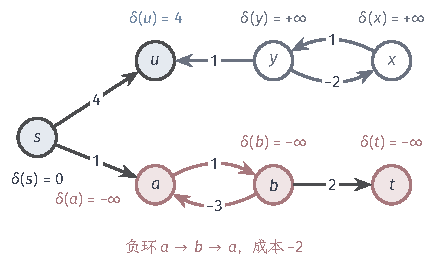
\includegraphics[width=73.801mm]{figures/01-basic-mathematics/04-graphs/tikz/c3-distance-outcomes/figure.pdf}
  \caption{单源最短路的三类结果同处一图（源点为$s$，弧旁数字为长度）。$a\to b\to a$的成本为$1-3=-2$，是从$s$可达的负环，环上的$a,b$及其后继$t$的距离为$-\infty$（红色）；旁支$u$不能从该负环到达，距离为有限值$4$（蓝色）；负环$x\to y\to x$从$s$不可达，$x,y$的距离为$+\infty$（灰色），弧$y\to u$也不会改变$u$的距离。}
  \label{fig:graph-opt-distance-outcomes}
\end{figure}

无向图中的负边需要特别注意。把无向边$\{u,v\}$换成两条同长的反向弧$u\to v$与$v\to u$以后，一条长为负的无向边自己就构成负环：沿它走过去再走回来，成本是两倍的负长度。因此，含负边的无向图不能直接套用本章的有向算法；本章默认讨论有向图，无向边只在长度非负时换成一对反向弧。

\section{距离标签与松弛}
\label{sec:graph-opt-relaxation}

三种算法都不直接枚举行走，而是为每个顶点保存一个当前已知的最好成本，在发现更好的路线时更新它。设想已经知道一条从$s$到$u$、成本为$d(u)$的路线，又有弧$u\to v$，那么把这条弧接在路线末尾，就得到一条到$v$、成本为$d(u)+\ell_{u,v}$的路线。如果它比$v$目前记录的成本更低，就应该改用它。

\paragraph{松弛操作}
为每个顶点$v$保存一个\term{距离标签}（distance label）$d(v)\in\mathbb R\cup\{+\infty\}$和一个前驱$p(v)$。初始时令$d(s)=0$，其余顶点$d(v)=+\infty$，前驱为空。对一条弧$u\to v$执行\term{松弛}（relaxation），是指比较当前标签$d(v)$与候选值$d(u)+\ell_{u,v}$：若$d(u)<+\infty$且
\begin{equation}
  d(u)+\ell_{u,v}<d(v),
  \label{eq:graph-opt-relaxation}
\end{equation}
就令$d(v)\leftarrow d(u)+\ell_{u,v}$、$p(v)\leftarrow u$；否则什么也不做。只有严格改善时才更新，因而标签只会下降，不会上升。

图~\ref{fig:graph-opt-relaxation}画出一次松弛的两种结果：候选值$5$小于原标签$8$时，标签与前驱一起改写；原标签已是$4$时，两者都不变。距离数组和前驱数组必须同步修改：如果只改距离而不改前驱，回溯得到的路线成本就不再等于标签。

\begin{figure}[!htb]
  \centering
  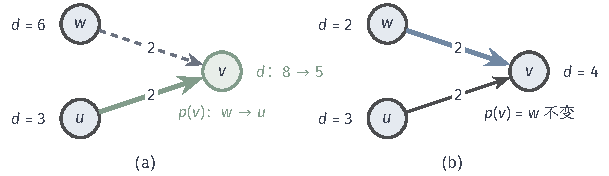
\includegraphics[width=102.993mm]{figures/01-basic-mathematics/04-graphs/tikz/c3-relaxation/figure.pdf}
  \caption{对弧$u\to v$松弛（顶点旁为当前标签，弧旁为长度）。(a) 候选值$d(u)+\ell_{u,v}=3+2=5$小于原标签$8$，标签改为$5$，前驱由$w$改为$u$（绿色表示被改善的标签与新的前驱弧，虚线为被替换的旧前驱弧）。(b) 原标签为$4$，候选值$5$不能改善，标签与前驱都不变。}
  \label{fig:graph-opt-relaxation}
\end{figure}

\paragraph{上界不变量}
松弛只从有限标签出发延长路线，由此得到所有算法共用的一个不变量：\emph{每个有限标签$d(v)$都等于某条从$s$到$v$的行走的成本}。初始时只有$d(s)=0$有限，对应零步行走。若松弛把$d(v)$改为$d(u)+\ell_{u,v}$，则把$u$的那条行走接上弧$u\to v$，就得到成本恰为新标签的行走。由此立即得到$d(v)\geq\delta(v)$：标签永远是真实距离的上界。后面每种算法要做的，都是说明在适当的条件下，这个上界最终会降到$\delta(v)$。

能否反过来，直接解一组方程得到距离？若没有可达负环，真实距离满足一组局部等式：$\delta(s)=0$，并且对每个可达的$v\neq s$，有
\[
  \delta(v)=\min_{u\to v}\{\delta(u)+\ell_{u,v}\}.
\]
这只是说最短路的最后一条弧总来自某个前驱。

但满足这组等式的数组不一定就是距离。设$s\to a$长$5$，$a\to b$与$b\to a$长都为$0$，则对任意$c\leq5$，取$D(s)=0$、$D(a)=D(b)=c$都满足
\[
  D(a)=\min\{D(s)+5,\ D(b)+0\}=c,\qquad D(b)=D(a)+0=c,
\]
而真实距离是$\delta(a)=\delta(b)=5$。这里的零成本环让$a,b$互相“支撑”着一个过低的值，却没有任何实际路线达到它。

所以算法不能只去求解局部等式，而要从“源为零、其余为无穷”的初值出发，只沿实际路线下调标签：初值保证标签不会无中生有，松弛保证每个标签都有路线见证。松弛按什么次序进行、何时可以停止，则由各算法分别规定。

三种算法都同时保存标签与前驱。前驱记录达到当前上界的最后一条弧，用于事后恢复路线，但只在标签不再变化以后才能放心回溯：在一般有环图中，计算中途的前驱指针可能尚未形成从$s$出发的树；若存在可达负环，前驱指针甚至可能首尾相接成环。

\section{有向无环图上的最短路}
\label{sec:graph-opt-dag-shortest-path}

\subsection{问题与思路}

输入限定为有向无环图，弧长仍可为任意实数。在一般的图中，一个顶点的标签可能在它的出弧已被松弛之后才下降，这时它的后继也必须随之更新。有向无环图没有这个问题：第~\ref{sec:graph-topological-order}节说明，有限有向无环图存在拓扑序，使每条弧的起点排在终点之前。按拓扑序处理顶点，轮到$v$时，所有指向$v$的弧都已被松弛，$v$的标签此后不会再变，于是可以放心地用它去松弛$v$的出弧。

\subsection{算法实现}

拓扑序在松弛开始前一次求出，它只规定处理次序，运行中不再改变，因此不计入算法状态。算法维护三项状态：
\begin{itemize}
  \item 距离标签$d(v)$：初值$d(s)=0$，其余为$+\infty$；
  \item 前驱$p(v)$：初值为空；
  \item 位置$i$：下一个待处理的顶点在拓扑序中的序号，初值为$1$。
\end{itemize}
每一步处理拓扑序中的第$i$个顶点$v_i$：若$d(v_i)<+\infty$，对它的每条出弧执行松弛，否则它给不出有限候选，直接跳过；然后令$i\gets i+1$。处理完$v_n$后停止，再沿前驱恢复路线。

\begin{algorithm}[有向无环图上的最短路]
\label{alg:graph-opt-dag-shortest-path}
输入：有限有向无环图、弧长$\ell_{u,v}\in\mathbb R$、源点$s$。输出：全部距离$\delta(v)$与前驱$p(v)$。
\begin{enumerate}
  \item 求一个拓扑序$v_1,\ldots,v_n$；令$d(s)=0$，其余$d(v)=+\infty$，前驱为空。
  \item 按$i=1,\ldots,n$的顺序处理$v_i$：若$d(v_i)<+\infty$，对其每条出弧$v_i\to w$执行松弛。
  \item 对标签有限的顶点，沿前驱从终点退回$s$再反转，得到一条最短路；标签为$+\infty$的顶点报告不可达。
\end{enumerate}
\end{algorithm}

\paragraph{执行过程}
下面用一张四点图逐步演示，它的五条弧长为：
\[
  \ell_{s,a}=2,\quad\ell_{s,b}=5,\quad\ell_{a,b}=-1,\quad\ell_{a,t}=5,\quad\ell_{b,t}=2.
\]
这张图没有有向环，拓扑序可取$(s,a,b,t)$。初始标签为
\[
  (d(s),d(a),d(b),d(t))=(0,+\infty,+\infty,+\infty),
\]
前驱全为空。按拓扑序逐个处理顶点，松弛它的出弧：
\begin{itemize}
  \item 处理$s$：$a$由$+\infty$改为$0+2=2$，$b$由$+\infty$改为$0+5=5$，前驱都记为$s$，标签变为$(0,2,5,+\infty)$。
  \item 处理$a$：候选$2+(-1)=1<5$，$b$改为$1$、前驱改为$a$；$t$由$+\infty$改为$2+5=7$、前驱记为$a$。标签变为$(0,2,1,7)$。
  \item 处理$b$：候选$1+2=3<7$，$t$改为$3$、前驱改为$b$，标签变为$(0,2,1,3)$。
  \item 处理$t$：没有出弧，标签不变。
\end{itemize}
扫描结束时前驱为$p(a)=s$、$p(b)=a$、$p(t)=b$。从$t$回溯得到最短路$s\to a\to b\to t$，成本为
\[
  \ell_{s,a}+\ell_{a,b}+\ell_{b,t}=2-1+2=3.
\]
图~\ref{fig:graph-opt-dag-labels}记录了各标签的变化次序。

\begin{figure}[!htb]
  \centering
  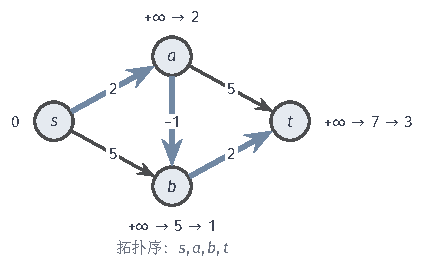
\includegraphics[width=71.635mm]{figures/01-basic-mathematics/04-graphs/tikz/c3-dag-labels/figure.pdf}
  \caption{按拓扑序$(s,a,b,t)$在有向无环图上松弛。顶点旁列出标签的变化次序，例如$b$先由处理$s$得到$5$，再由处理$a$改为$1$；蓝色粗弧是最终前驱弧，组成最短路$s\to a\to b\to t$（成本$3$）。负长度弧$a\to b$并不妨碍计算，因为正确性只依赖无环次序。}
  \label{fig:graph-opt-dag-labels}
\end{figure}

\subsection{算法分析}

\paragraph{正确性}
一遍扫描之所以够用，是因为处理到某个顶点时，所有可能到达它的路线都已考虑过。

\begin{theorem}[有向无环图上最短路的正确性]
\label{thm:graph-opt-dag-shortest-path}
设$\mathcal G$是有限有向无环图，弧长为任意实数。算法~\ref{alg:graph-opt-dag-shortest-path}结束时，对每个顶点$v$都有$d(v)=\delta(v)$；其中$\delta(v)=+\infty$当且仅当$v$从$s$不可达，其余$\delta(v)$均为有限值。
\end{theorem}

\begin{proof}
有向无环图中的行走不会重复顶点，因此每条行走都是简单路径，只有有限条，$\delta(v)$只可能是$+\infty$或有限值。松弛只改变弧终点的标签，而指向$v$的弧都从拓扑序中排在$v$之前的顶点出发，所以轮到$v$时它的标签已经不再改变。下面对拓扑序归纳，证明轮到$v$时$d(v)=\delta(v)$。

排在$s$之前的顶点从$s$不可达，它们的标签保持$+\infty$，与距离一致。对$v=s$，不存在回到$s$的非零步行走，故$\delta(s)=0=d(s)$。

设$v$排在$s$之后，并且此前的顶点都已满足结论。若$v$不可达，则它的标签不可能变为有限值，因为有限标签总对应一条实际行走。若$v$可达，任取一条$s$到$v$的路径，设其最后一条弧为$u\to v$，则$u$排在$v$之前，路径前缀的成本不小于$\delta(u)$，归纳假设给出$\delta(u)=d(u)$。处理$u$时弧$u\to v$已被松弛，因而
\[
  d(v)\leq d(u)+\ell_{u,v}=\delta(u)+\ell_{u,v}\leq\text{该路径的成本}.
\]
路径是任取的，所以$d(v)\leq\delta(v)$。结合标签不变量$d(v)\geq\delta(v)$，得$d(v)=\delta(v)$。
\end{proof}

证明中只用到“前驱先于后继处理”，没有用到边长的符号，所以负长度弧不会造成任何问题；反过来，图中只要有一个有向环就没有拓扑序，算法无法开始，此时要改用后面两种算法。

\paragraph{复杂度}
求拓扑序需要$O(n+a)$时间，之后每个顶点处理一次、每条弧松弛一次，总时间为$O(n+a)$，标签、前驱与拓扑序共占$O(n)$额外空间。

\subsection{编辑距离}

许多递推问题的状态之间天然形成有向无环图：每个状态的最优值，由能一步转来的前面状态加上这一步的代价取最小得到。这正是按拓扑序松弛的最短路问题，编辑距离是一个典型例子。

比较两段序列时，常问把序列$\bm a=(a_1,\ldots,a_p)$改写成$\bm b=(b_1,\ldots,b_q)$最少需要多少次单元素操作，允许的操作是插入一个元素、删除一个元素和把一个元素替换为另一个。

以$(i,j)$表示“已把$\bm a$的前$i$个元素改写成$\bm b$的前$j$个元素”这一状态，最后一步只有三种可能：删去$a_i$，从$(i-1,j)$而来，成本为$1$；插入$b_j$，从$(i,j-1)$而来，成本为$1$；让$a_i$对应$b_j$，从$(i-1,j-1)$而来，相同时成本为$0$，不同时为一次替换，成本为$1$。

于是最少操作数$E(i,j)$满足
\begin{equation}
  E(i,j)=\min\bigl\{E(i-1,j)+1,\ E(i,j-1)+1,\ E(i-1,j-1)+\mathbb I\{a_i\neq b_j\}\bigr\},
  \label{eq:graph-opt-edit-distance}
\end{equation}
边界为$E(i,0)=i$、$E(0,j)=j$，其中$\mathbb I\{\cdot\}$在条件成立时取$1$、否则取$0$。

每条状态弧都使$i+j$增加，所以状态图没有有向环，$E(p,q)$就是从$(0,0)$到$(p,q)$的最短路距离，称为两段序列的\term{编辑距离}（edit distance）。

按$i+j$递增或逐行的顺序计算，正是在按拓扑序松弛。例如$\bm a=(A,B)$、$\bm b=(A,C,B)$时，逐行计算得到表~\ref{tab:graph-opt-edit-distance}，沿“匹配$A$、插入$C$、匹配$B$”得到距离$E(2,3)=1$。

全表连同前驱需要$O(pq)$时间与空间；只要距离值时保留相邻两行即可。若给插入、删除和替换配上不同的成本，只需改变相应状态弧的长度，状态图仍然无环，计算次序不变。

\begin{table}[!htb]
  \centering
  \begin{tabular}{@{}ccccc@{}}
    \toprule
    & $j=0$ & $j=1$（$A$） & $j=2$（$C$） & $j=3$（$B$） \\
    \midrule
    $i=0$ & $0$ & $1$ & $2$ & $3$ \\
    $i=1$（$A$） & $1$ & $0$ & $1$ & $2$ \\
    $i=2$（$B$） & $2$ & $1$ & $1$ & $1$ \\
    \bottomrule
  \end{tabular}
  \caption{$\bm a=(A,B)$改写为$\bm b=(A,C,B)$的编辑距离表。第$i$行第$j$列为$E(i,j)$，按式~\eqref{eq:graph-opt-edit-distance}逐行计算；右下角$E(2,3)=1$。}
  \label{tab:graph-opt-edit-distance}
\end{table}

\section{Bellman--Ford算法}
\label{sec:graph-opt-bellman-ford}

\subsection{问题与思路}

一般的有向图可能有环，没有拓扑序可用，一遍扫描不够。最直接的补救是反复扫描全部弧，让后来的改善继续向后传递，直到标签不再变化。为了说清每一轮扫描得到了什么，考虑各轮彼此分开的同步版本：第$k$轮只读取第$k-1$轮结束时的标签。这样，第$k$轮的标签恰好考虑了至多$k$条弧的路线；不受负环影响的顶点由至多$n-1$条弧的简单路径达到，所以$n-1$轮就够了。完成这些轮次后再扫描一次，仍能改善的弧就暴露了负环的影响。

\subsection{算法实现}

同步版本的第$k$轮对每个顶点比较“沿用旧值”与“在上一轮的某条路线后再接一条弧”：
\begin{equation}
  d^{(k)}(v)=\min\Bigl\{d^{(k-1)}(v),\ \min_{u\to v}\bigl(d^{(k-1)}(u)+\ell_{u,v}\bigr)\Bigr\},\qquad k=1,2,\ldots,
  \label{eq:graph-opt-bellman-ford}
\end{equation}
没有入弧时内层最小值取$+\infty$。算法维护四项状态：
\begin{itemize}
  \item 两份标签数组$d^{(k-1)}$与$d^{(k)}$：本轮只读前者、只写后者，初值$d^{(0)}(s)=0$，其余为$+\infty$；
  \item 前驱$p(v)$：最近一次改善$d(v)$时提供候选值的顶点，初值为空；
  \item 轮次$k$：已完成的轮数，初值为$0$；
  \item 改善标记：本轮有无标签改变。
\end{itemize}
每一轮依次做三件事：
\begin{itemize}
  \item 复制：令$k\gets k+1$，把$d^{(k-1)}$复制为$d^{(k)}$，改善标记置为否。
  \item 逐弧更新：对每条起点标签有限的弧$u\to v$，若$d^{(k-1)}(u)+\ell_{u,v}<d^{(k)}(v)$，就令$d^{(k)}(v)\gets d^{(k-1)}(u)+\ell_{u,v}$、$p(v)\gets u$，并记下有改善。扫描完全部弧，$d^{(k)}$恰为式~\eqref{eq:graph-opt-bellman-ford}的右端。
  \item 停止判断：若$k=n-1$或本轮无改善，停止递推；否则进入下一轮。
\end{itemize}
递推停止后，固定此时的标签$d$，分两步判别负环的影响：
\begin{itemize}
  \item 找种子：起点标签有限、仍满足$d(u)+\ell_{u,v}<d(v)$的弧$u\to v$，其终点称为种子。递推提前停止时没有种子。
  \item 标记：从全部种子出发沿出弧遍历，把到达的顶点标记为$-\infty$。
\end{itemize}
其余顶点中，标签为$+\infty$的报告不可达，标签有限的以标签为距离。

\begin{algorithm}[Bellman--Ford算法]
\label{alg:graph-opt-bellman-ford}
输入：有向图的出邻接表与弧长$\ell$，起点$s$。输出：每个顶点的距离或“不可达”“$-\infty$”，以及前驱。
\begin{enumerate}
  \item 置$d^{(0)}(s)=0$，其余$d^{(0)}(v)=+\infty$，前驱为空，$k=0$。
  \item 令$k\gets k+1$，把$d^{(k-1)}$复制为$d^{(k)}$。对每条$d^{(k-1)}(u)<+\infty$的弧$u\to v$，若$d^{(k-1)}(u)+\ell_{u,v}<d^{(k)}(v)$，置$d^{(k)}(v)=d^{(k-1)}(u)+\ell_{u,v}$、$p(v)=u$。
  \item 若本轮有标签改善且$k<n-1$，回到第2步；否则记$d=d^{(k)}$。
  \item 把满足$d(u)<+\infty$且$d(u)+\ell_{u,v}<d(v)$的弧$u\to v$的终点作为种子，从全部种子沿出弧遍历，到达的顶点标为$-\infty$；其余顶点按$d$报告距离或不可达。
\end{enumerate}
\end{algorithm}

\paragraph{执行过程}
上一节的四点图没有环，看不出反复扫描的必要。图~\ref{fig:graph-opt-bellman-ford-rounds}换用一个有环的例子，它有五个顶点和六条弧，弧长为：
\[
  \begin{gathered}
    \ell_{s,t}=6,\quad\ell_{s,b}=2,\quad\ell_{b,c}=3,\\
    \ell_{c,a}=-4,\quad\ell_{a,t}=2,\quad\ell_{t,b}=1.
  \end{gathered}
\]
其中$b\to c\to a\to t\to b$构成一个环，成本为$3-4+2+1=2$，不是负环。按式~\eqref{eq:graph-opt-bellman-ford}逐轮计算，各轮标签见表~\ref{tab:graph-opt-bellman-ford-rounds}。

第$1$轮只能用一条弧：$t$由$s$得到$6$，$b$由$s$得到$2$，其余仍为$+\infty$。
\begin{BookInlineFigure}
  \centering
  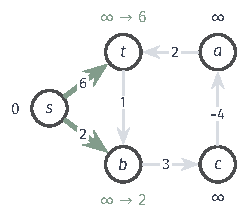
\includegraphics[width=40.771mm]{figures/03-graphs/02-combinatorial-optimization/tikz/reading-steps/bellman-ford-round-1.pdf}
  \caption{Bellman--Ford第$1$轮结束。本轮只能沿从$s$出发的单条弧产生有限候选。弧旁数字是弧长，顶点旁是标签；绿色弧与数字表示本轮改善，蓝色弧表示此前保留的前驱。}
  \label{fig:graph-opt-bellman-ford-rounds}
\end{BookInlineFigure}

第$2$轮：$c$经$b$得到$2+3=5$。$a\to t$与$c\to a$的起点在上一轮还是$+\infty$，不产生候选。
\begin{BookInlineFigure}
  \centering
  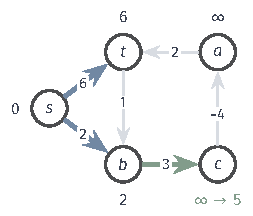
\includegraphics[width=42.774mm]{figures/03-graphs/02-combinatorial-optimization/tikz/reading-steps/bellman-ford-round-2.pdf}
  \caption{第$2$轮：改善从$b$传到$c$，得到$d(c)=5$。本轮仍读取上一轮的标签，因此不能立刻沿$c\to a$继续传递。}
  \label{fig:graph-opt-bellman-ford-rounds-2}
\end{BookInlineFigure}

第$3$轮：$a$经$c$得到$5-4=1$，对应三弧路线$s\to b\to c\to a$。
\begin{BookInlineFigure}
  \centering
  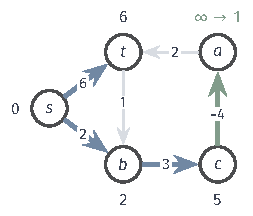
\includegraphics[width=42.774mm]{figures/03-graphs/02-combinatorial-optimization/tikz/reading-steps/bellman-ford-round-3.pdf}
  \caption{第$3$轮：沿$c\to a$得到$d(a)=1$。此前$t$的标签仍为直达路线的成本$6$。}
  \label{fig:graph-opt-bellman-ford-rounds-3}
\end{BookInlineFigure}

第$4$轮：$t$经$a$降到$1+2=3$，前驱由$s$改为$a$，对应四弧路线$s\to b\to c\to a\to t$，比直达的$s\to t$便宜。
\begin{BookInlineFigure}
  \centering
  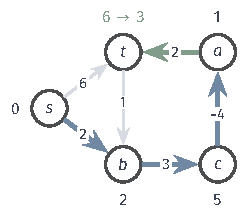
\includegraphics[width=40.771mm]{figures/03-graphs/02-combinatorial-optimization/tikz/reading-steps/bellman-ford-round-4.pdf}
  \caption{第$4$轮：沿$a\to t$把$d(t)$由$6$降为$3$，并改写$t$的前驱。蓝绿弧组成最终最短路径树。}
  \label{fig:graph-opt-bellman-ford-rounds-4}
\end{BookInlineFigure}

此时$k=4=n-1$，递推停止。再检查全部弧，没有一条还能改善，因而没有种子，最终距离为$(s,a,b,c,t)=(0,1,2,5,3)$。

这个例子恰好用满了$n-1$轮，因为$t$的最短路含$4$条弧；每一行都是“至多$k$条弧”的最优值，例如$d^{(3)}(t)=6$只计入了单弧路线$s\to t$。改善沿环$b\to c\to a\to t$传递了一圈，但回到$b$时，候选$3+1=4$不小于$2$，传递就此停止：环的成本非负，绕圈不会更便宜。


\begin{table}[!htb]
  \centering
  \begin{tabular}{cccccc}
    \toprule
    轮次$k$ & $d^{(k)}(s)$ & $d^{(k)}(a)$ & $d^{(k)}(b)$ & $d^{(k)}(c)$ & $d^{(k)}(t)$ \\
    \midrule
    $0$ & $0$ & $+\infty$ & $+\infty$ & $+\infty$ & $+\infty$ \\
    $1$ & $0$ & $+\infty$ & $2$（$s$） & $+\infty$ & $6$（$s$） \\
    $2$ & $0$ & $+\infty$ & $2$ & $5$（$b$） & $6$ \\
    $3$ & $0$ & $1$（$c$） & $2$ & $5$ & $6$ \\
    $4$ & $0$ & $1$ & $2$ & $5$ & $3$（$a$） \\
    \bottomrule
  \end{tabular}
  \caption{同步Bellman--Ford在图~\ref{fig:graph-opt-bellman-ford-rounds}的含环图上的逐轮标签。第$k$行是至多$k$条弧的最小成本，括号内为该轮改变标签时的前驱。}
  \label{tab:graph-opt-bellman-ford-rounds}
\end{table}

负环存在时，标签不会停下来。回到图~\ref{fig:graph-opt-distance-outcomes}。该图有$7$个顶点，同步计算$6$轮，各轮标签见表~\ref{tab:graph-opt-bellman-ford-negative}。$u$在第$1$轮得到$4$后不再变化，$x,y$始终为$+\infty$；而$a,b,t$的标签每隔一两轮就再降一次，第$6$轮停在$-3,-2,2$。这几个数只反映绕圈到第$6$轮时标签降到了哪里，并不是任何意义下的距离。

此时检查全部弧，$b\to a$与$b\to t$的候选分别为
\[
  -2-3=-5<-3,\qquad -2+2=0<2,
\]
两条弧仍可改善，种子是$a$与$t$；其余弧都不能改善。从种子沿出弧遍历，标记出$\{a,b,t\}$。算法报告$u$的距离为$4$，$a,b,t$为$-\infty$，$x,y$不可达，与前面的分析一致。

\begin{table}[!htb]
  \centering
  \begin{tabular}{cccccc}
    \toprule
    轮次$k$ & $d^{(k)}(s)$ & $d^{(k)}(u)$ & $d^{(k)}(a)$ & $d^{(k)}(b)$ & $d^{(k)}(t)$ \\
    \midrule
    $0$ & $0$ & $+\infty$ & $+\infty$ & $+\infty$ & $+\infty$ \\
    $1$ & $0$ & $4$ & $1$ & $+\infty$ & $+\infty$ \\
    $2$ & $0$ & $4$ & $1$ & $2$ & $+\infty$ \\
    $3$ & $0$ & $4$ & $-1$ & $2$ & $4$ \\
    $4$ & $0$ & $4$ & $-1$ & $0$ & $4$ \\
    $5$ & $0$ & $4$ & $-3$ & $0$ & $2$ \\
    $6$ & $0$ & $4$ & $-3$ & $-2$ & $2$ \\
    \bottomrule
  \end{tabular}
  \caption{同步Bellman--Ford在图~\ref{fig:graph-opt-distance-outcomes}上的逐轮标签（$x,y$各轮均为$+\infty$，未列出）。$u$在第$1$轮后稳定；可达负环$a\to b\to a$使$a,b,t$的标签持续下降。}
  \label{tab:graph-opt-bellman-ford-negative}
\end{table}

\paragraph{就地更新}
常见的实现不复制数组，而是在同一个数组上逐弧松弛，一轮中刚改善的标签可以立即被同一轮后面的弧使用，称为就地更新。

扫描次序会影响所需轮数。按$s\to t$、$s\to b$、$b\to c$、$c\to a$、$a\to t$、$t\to b$的顺序扫描上例，第一轮就依次得到$t=6$、$b=2$、$c=5$、$a=1$，并把$t$降到$3$，即全部最终标签，第二轮无改善即可停止。若按相反的顺序扫描，每轮只能把改善推进一步，仍要四轮。

它的停止规则与负环检测方式和同步版本相同，只是“第$k$轮”的含义变了。

\subsection{算法分析}

\paragraph{正确性}
分析从同步版本出发，因为它的标签有一个清楚的含义。

\begin{lemma}[同步标签的含义]
\label{lem:graph-opt-bellman-ford-k-arcs}
对每个$k\geq0$与每个顶点$v$，$d^{(k)}(v)$等于从$s$到$v$、至多含$k$条弧的全部行走的最小成本；没有这样的行走时为$+\infty$。
\end{lemma}

\begin{proof}
对$k$归纳。$k=0$时，至多零条弧的行走只有$s$处的零步行走，与$d^{(0)}$一致。设结论对$k-1$成立。一条至多含$k$条弧、到达$v$的行走，要么至多含$k-1$条弧，其成本不小于$d^{(k-1)}(v)$；要么恰含$k$条弧，去掉最后一条弧$u\to v$后剩下至多$k-1$条弧、到达$u$的前缀，其成本不小于$d^{(k-1)}(u)+\ell_{u,v}$。所以全部候选的最小值不小于式~\eqref{eq:graph-opt-bellman-ford}的右端。反过来，右端每一项都由归纳假设对应一条至多$k$条弧的行走，最小值能够达到。故两者相等。
\end{proof}

由此先得到轮数上界。对不受可达负环影响的顶点$v$，第~\ref{sec:graph-opt-path-cost}节说明$\delta(v)$由一条简单路径达到，而简单路径至多经过$n$个顶点、含$n-1$条弧。由引理~\ref{lem:graph-opt-bellman-ford-k-arcs}，第$n-1$轮已经计入这条路径，所以$d^{(n-1)}(v)=\delta(v)$。若某一整轮没有任何标签改变，则此后各轮的输入都相同，标签不会再变，提前停止不影响结果；此时由下面的定理，图中不存在可达负环。

就地更新得到的标签仍是真实行走的成本，又对每轮都不高于同步版本的标签（对轮数归纳即可），所以$n-1$轮的上界照样成立。但“第$k$轮标签恰为至多$k$条弧的最优值”这一解释只属于同步版本，不能原样套在就地更新上：同一轮内的改善可能已经串起了多条弧。

\paragraph{负环的判别}
$n-1$轮之后的种子与遍历恰好找出了全部距离为$-\infty$的顶点。

\begin{theorem}[Bellman--Ford算法对三类结果的判定]
\label{thm:graph-opt-bellman-ford-negative-cycles}
在同步递推的$n-1$轮之后按上述方法标记，被标记的顶点恰好是$\delta(v)=-\infty$的顶点；其余顶点中，$d^{(n-1)}(v)=+\infty$的不可达，$d^{(n-1)}(v)$有限的满足$d^{(n-1)}(v)=\delta(v)$。
\end{theorem}

\begin{proof}
先证每个种子$v$都满足$\delta(v)=-\infty$。由引理~\ref{lem:graph-opt-bellman-ford-k-arcs}，$v$可改善说明$d^{(n)}(v)<d^{(n-1)}(v)$，即存在一条恰含$n$条弧的行走，比所有至多$n-1$条弧的行走都便宜。

含$n$条弧的行走经过$n+1$个顶点位置，必有顶点重复，从中可以切出一段闭行走$C$。若$C$的成本非负，删去它会得到弧更少、成本不更高的行走，与上述“更便宜”矛盾；故$C$的成本为负，由第~\ref{sec:graph-opt-path-cost}节的分解，$C$中含有一个负环。这个负环位于一条从$s$出发、到达$v$的行走上，所以$\delta(v)=-\infty$。从种子沿出弧能到达的顶点也能从同一个负环到达，因而被标记的顶点距离都是$-\infty$。

再证每个$\delta(v)=-\infty$的顶点都会被标记。此时存在从$s$可达的负环$C=(c_0,c_1,\ldots,c_k=c_0)$能到达$v$。$C$上的顶点从$s$可达，可达顶点至多经$n-1$条弧到达，所以它们的标签有限。若$C$上没有一条弧可改善，则对每条环弧都有
\[
  d(c_{r})\leq d(c_{r-1})+\ell_{c_{r-1},c_r},\qquad r=1,\ldots,k.
\]
沿环把这$k$个不等式相加，两侧的标签之和恰好相消，得到$0\leq\ell(C)<0$，矛盾。因此$C$上至少有一个种子，而$v$能从$C$到达，必然被遍历标记。

最后，未被标记且可达的顶点不受任何可达负环影响，前面已说明$d^{(n-1)}(v)=\delta(v)$；不可达顶点的标签始终为$+\infty$。
\end{proof}

\paragraph{复杂度}
每轮逐弧扫描一次，用时$O(a)$，至多$n-1$轮，再加上一轮检测与一次遍历，总时间为$O(na)$。同步版本每轮还要复制标签数组，另需$O(n)$时间，合计至多$O(n^2)$；就地更新省去这部分。只保存当前和上一轮的标签时，工作状态为$O(n)$。

\paragraph{路线恢复}
若要按引理~\ref{lem:graph-opt-bellman-ford-k-arcs}的含义回溯“至多$k$条弧”的最优路线，就需要保存每一轮的前驱$p^{(k)}(v)$，记录可达$O(n^2)$条。只保存一份前驱数组时，也可以回溯有限距离的顶点，但要说明这份前驱与递推相容。

设$v$未被标记且标签有限，若$p(v)=u$，则$u\to v$是一条弧，$u$也不会被标记，否则$v$能从负环到达。设置$p(w)=u$时，$d(w)$等于$u$此前某一时刻的标签加上$\ell_{u,w}$；标签只降不升，$d(w)$再下降时前驱又会改写，所以任一时刻每条前驱弧都满足
\[
  d(p(w))+\ell_{p(w),w}\leq d(w).
\]

前驱指针在未标记顶点之间不会成环：若成环，考察环上最后被设置的那个指针，在它被设置之前，环上其余前驱弧都满足上述不等式，而这条弧满足严格不等式，沿环相加，标签相消，得到环的成本为负；这个负环从$s$可达，又能沿前驱弧到达$v$，与$v$未被标记矛盾。于是从$v$沿前驱必能回到$s$。把沿途的不等式相加，所得路线的成本不超过$d(v)=\delta(v)$，因而恰好是一条最短路。

对标为$-\infty$的顶点，算法给出的不是一条“最短路”，而是负环的证据：一个种子、一条从$s$到负环的行走与一条从负环到该顶点的行走。

\section{Dijkstra算法}
\label{sec:graph-opt-dijkstra}

\subsection{问题与思路}

Bellman--Ford算法要反复扫描全部弧，因为一个标签随时可能再被改小。若边长都非负，情况就不同了：在尚未确定的顶点中，标签最小的那个已经不可能再被改小，因为任何绕道而来的路线都要先经过某个标签不更小的顶点，后半程又不会让成本下降。Dijkstra算法利用这一点，每次把这样一个顶点永久确定下来，只松弛它的出弧，于是每条弧只需松弛一次。

Dijkstra算法所需的条件是从源点可达部分的弧长都非负。全图非负是便于检查的充分条件；从$s$到达不了的区域即使有负边，也不影响本次查询。在这一条件下，从$s$可达的部分不含负环，所有距离都是$+\infty$或有限值，输出只有两类。

\subsection{算法实现}

\paragraph{优先队列的数据结构}
取出标签最小的未确定顶点、在标签下降时调整它的位置，都由以标签为键的优先队列完成，常见的实现有两种。一种是支持“降键”的索引堆，每个顶点在堆中只有一个条目，标签改善时原地下调它的键。另一种不降键，标签改善时直接插入一个新条目$(d(v),v)$，旧条目留在堆中；出队时若发现该顶点已经确定，说明这是过期条目，直接丢弃。两种实现的输出相同，区别只在队列规模与操作次数。

\paragraph{Dijkstra算法的实现}
算法维护四项状态：
\begin{itemize}
  \item 距离标签$d(v)$：初值$d(s)=0$，其余为$+\infty$；
  \item 前驱$p(v)$：初值为空；
  \item 已确定集合$R$：标签已永久确定的顶点，初值为空集；
  \item 优先队列：以标签为键存放标签有限的未确定顶点，初值只含$s$。
\end{itemize}
每一步做两件事：
\begin{itemize}
  \item 确定：取出队列中标签最小的顶点$u$，把它加入$R$；
  \item 松弛：对$u$通往$R$外的每条出弧执行松弛，标签改善时相应调整队列。
\end{itemize}
队列中不再有标签有限的未确定顶点时停止。

\begin{algorithm}[Dijkstra算法]
\label{alg:graph-opt-dijkstra}
输入：有限有向图、源点$s$，从$s$可达部分的弧长非负。输出：全部距离$\delta(v)$与前驱$p(v)$。
\begin{enumerate}
  \item 令$d(s)=0$，其余$d(v)=+\infty$，$R=\varnothing$。
  \item 当存在标签有限的未确定顶点时，取出其中标签最小的$u$，把$u$加入$R$。
  \item 对$u$的每条出弧$u\to v$，若$v\notin R$，执行松弛；标签改善时更新优先队列中$v$的键。
  \item 结束时，$R$中顶点的标签即为距离，其余顶点不可达。
\end{enumerate}
\end{algorithm}

\paragraph{执行过程}
把四点图中$a\to b$的长度由$-1$改为$1$，全部弧长非负，Dijkstra算法适用。表~\ref{tab:graph-opt-dijkstra-trace}列出每次出队后的状态。

第$1$步取出$s$，松弛得$d(a)=2$、$d(b)=5$，前驱都是$s$。
\begin{BookInlineFigure}
  \centering
  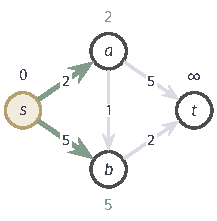
\includegraphics[width=36.784mm]{figures/03-graphs/02-combinatorial-optimization/tikz/reading-steps/dijkstra-step-1.pdf}
  \caption{Dijkstra第$1$步：取出$s$并松弛两条出弧。黄色是本次出队顶点，蓝底是已确定顶点；绿色标签和弧表示本次改善及新前驱。弧旁数字为长度，顶点旁为距离标签。}
  \label{fig:graph-opt-dijkstra-trace}
\end{BookInlineFigure}


第$2$步取出标签最小的$a$，候选$2+1=3<5$使$d(b)=3$、$p(b)=a$，候选$2+5=7$使$d(t)=7$、$p(t)=a$。
\begin{BookInlineFigure}
  \centering
  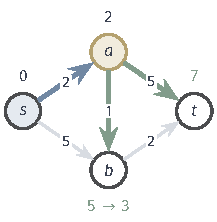
\includegraphics[width=36.784mm]{figures/03-graphs/02-combinatorial-optimization/tikz/reading-steps/dijkstra-step-2.pdf}
  \caption{第$2$步：确定$a$，经$a$把$b$的标签从$5$降为$3$，并首次到达$t$。已确定的$s,a$不再改写。}
  \label{fig:graph-opt-dijkstra-trace-2}
\end{BookInlineFigure}


第$3$步取出$b$，候选$3+2=5<7$使$d(t)=5$、$p(t)=b$。
\begin{BookInlineFigure}
  \centering
  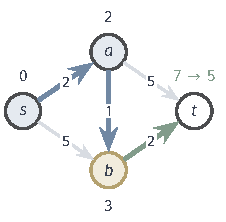
\includegraphics[width=38.347mm]{figures/03-graphs/02-combinatorial-optimization/tikz/reading-steps/dijkstra-step-3.pdf}
  \caption{第$3$步：确定$b$，经$b$把$t$的标签从$7$降为$5$。绿色弧$b\to t$替换此前的前驱弧$a\to t$。}
  \label{fig:graph-opt-dijkstra-trace-3}
\end{BookInlineFigure}


第$4$步取出$t$，它没有出弧，队列为空，停止。
\begin{BookInlineFigure}
  \centering
  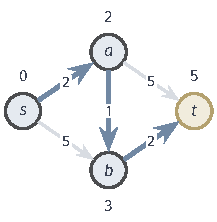
\includegraphics[width=36.784mm]{figures/03-graphs/02-combinatorial-optimization/tikz/reading-steps/dijkstra-step-4.pdf}
  \caption{第$4$步：确定$t$。最终前驱弧组成$s\to a\to b\to t$，各顶点标签均已等于最短距离。}
  \label{fig:graph-opt-dijkstra-trace-4}
\end{BookInlineFigure}


最终$\delta(a)=2$、$\delta(b)=3$、$\delta(t)=5$，从$t$沿前驱回溯得到$s\to a\to b\to t$。

图~\ref{fig:graph-opt-dijkstra-trace}至图~\ref{fig:graph-opt-dijkstra-trace-4}分别对应这四步：已确定集合$R$逐个向外扩张，每个顶点在出队时的标签都不再改变。

\begin{table}[!htb]
  \centering
  \begin{tabular}{@{}ccccccc@{}}
    \toprule
    步 & 出队 & $d(s)$ & $d(a)$ & $d(b)$ & $d(t)$ & $R$ \\
    \midrule
    初始 & — & $0$ & $+\infty$ & $+\infty$ & $+\infty$ & $\varnothing$ \\
    $1$ & $s$ & $0$ & $2$（$s$） & $5$（$s$） & $+\infty$ & $\{s\}$ \\
    $2$ & $a$ & $0$ & $2$ & $3$（$a$） & $7$（$a$） & $\{s,a\}$ \\
    $3$ & $b$ & $0$ & $2$ & $3$ & $5$（$b$） & $\{s,a,b\}$ \\
    $4$ & $t$ & $0$ & $2$ & $3$ & $5$ & $\{s,a,b,t\}$ \\
    \bottomrule
  \end{tabular}
  \caption{Dijkstra算法在非负四点图（$a\to b$长$1$，其余弧长同前）上的状态。每行是一次出队并松弛之后的标签与已确定集合，括号内为本步改变标签时的新前驱。}
  \label{tab:graph-opt-dijkstra-trace}
\end{table}


\subsection{算法分析}

\paragraph{正确性}
关键论断是：顶点被加入$R$的那一刻，它的标签已经等于真实距离，此后不再需要修正。证明的切入点是一条假设更短的路线上第一个尚未确定的顶点。

\begin{theorem}[Dijkstra算法的正确性]
\label{thm:graph-opt-dijkstra}
若从$s$可达部分的弧长都非负，则算法~\ref{alg:graph-opt-dijkstra}中每个顶点$u$被加入$R$时都有$d(u)=\delta(u)$；算法结束时未加入$R$的顶点从$s$不可达。
\end{theorem}

\begin{proof}
对加入$R$的次序归纳。第一个加入的是$s$，$d(s)=0=\delta(s)$，因为可达部分没有负环。设此前加入$R$的顶点都满足$d=\delta$，现在$u$被选出，且$d(u)<+\infty$。由标签不变量，$d(u)\geq\delta(u)$。假设$d(u)>\delta(u)$，取一条$s$到$u$、成本为$\delta(u)$的简单路径$P$。$P$从$s\in R$出发，到达$u\notin R$，所以沿$P$存在第一个不在$R$中的顶点$y$，记它在$P$上的前一个顶点为$x\in R$。

$x$加入$R$时弧$x\to y$已被松弛，此后标签只会下降。归纳假设给出$d(x)=\delta(x)$；而最短路的前缀仍是最短路，故$\delta(x)+\ell_{x,y}=\delta(y)$。于是
\[
  d(y)\leq d(x)+\ell_{x,y}=\delta(x)+\ell_{x,y}=\delta(y).
\]
$P$从$y$到$u$的后半段由可达部分的弧组成，长度非负，因而$\delta(y)\leq\delta(u)$。合起来得到
\[
  d(y)\leq\delta(y)\leq\delta(u)<d(u).
\]
但$y$也是未确定顶点，而算法选出的$u$在未确定顶点中标签最小，应有$d(u)\leq d(y)$，矛盾。所以$d(u)=\delta(u)$。

若算法停止时某个可达顶点$v$不在$R$中，取一条$s$到$v$的路径，同样找出第一个不在$R$中的顶点$y$及其前驱$x\in R$。松弛$x\to y$已使$d(y)$有限，算法便不会在此时停止，矛盾。
\end{proof}

\paragraph{适用范围}
证明中只有一步用到非负性：“后半段长度非负，所以$\delta(y)\leq\delta(u)$”。这一步失效时，算法确实会出错，即使图中没有负环。

下面的三弧图（图~\ref{fig:graph-opt-dijkstra-counterexample}）说明这一点，它的弧长为：
\[
  \ell_{s,a}=2,\quad\ell_{s,b}=5,\quad\ell_{b,a}=-4.
\]
处理$s$后，$a$的标签为$2$、$b$为$5$；算法选出标签较小的$a$并永久确定$d(a)=2$。随后处理$b$时，候选$5+(-4)=1$本可改善$a$，但$a$已在$R$中，不再更新。真实距离是$\delta(a)=1$，由路线$s\to b\to a$达到。

对照证明，这里的$y=b$、$u=a$，后半段$b\to a$为负，使$\delta(b)=5>\delta(a)=1$，“首个未确定顶点的标签不超过$\delta(u)$”不再成立。

\begin{figure}[!htb]
  \centering
  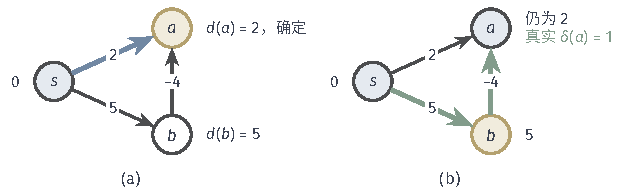
\includegraphics[width=105.583mm]{figures/01-basic-mathematics/04-graphs/tikz/c3-dijkstra-counterexample/figure.pdf}
  \caption{负边使Dijkstra算法过早确定标签。(a) 处理$s$后，$a$的标签$2$小于$b$的标签$5$，$a$被永久确定（黄色为当前出队顶点）。(b) 处理$b$时候选值$5-4=1$已无法改写$a$；真实最短路是$s\to b\to a$（绿色），成本$1$。图中没有负环，出错的原因是后半段弧$b\to a$为负。}
  \label{fig:graph-opt-dijkstra-counterexample}
\end{figure}

\paragraph{复杂度}
每个顶点至多出队一次，每条弧在其起点出队时松弛一次。用邻接表存储图、用支持降键的索引二叉堆存储未确定顶点时，取最小与降键各需$O(\log n)$时间，总时间为$O((n+a)\log n)$；标签、前驱、堆及其位置索引共占$O(n)$额外空间，图本身的存储另计。

不降键的实现每次改善插入一个条目，堆中至多有$a+1$个条目，操作时间为$O(\log a)=O(\log n)$，总时间仍为$O((n+a)\log n)$，但队列空间上界变为$O(a)$。稠密图上也可以不用堆，每次扫描数组找最小标签，总时间为$O(n^2+a)$。

\section{方法比较与结果检验}
\label{sec:graph-opt-shortest-path-comparison}

三种算法解决同一个单源问题，但对输入的要求不同。比较它们时应先问：图有没有有向环？可达部分有没有负长度弧？是否需要检测负环？然后才比较运行时间。表~\ref{tab:graph-opt-shortest-path-methods}汇总了这些区别。

\begin{table}[!htb]
  \centering
  \begin{tabular}{llll}
    \toprule
    & 有向无环图递推 & Bellman--Ford & Dijkstra \\
    \midrule
    图结构 & 无有向环 & 不限 & 不限 \\
    弧长 & 任意实数 & 任意实数 & 可达部分非负 \\
    标签修正 & 处理后不变 & 反复修正 & 出队后不变 \\
    负环 & 不会出现 & 检测并标记 & 条件排除 \\
    时间 & $O(n+a)$ & $O(na)$ & $O((n+a)\log n)$ \\
    正确性依据 & 拓扑序归纳 & 至多$k$弧递推 & 首个未定顶点 \\
    \bottomrule
  \end{tabular}
  \caption{三种单源最短路算法的比较（$n$为顶点数，$a$为弧数，邻接表存储）。}
  \label{tab:graph-opt-shortest-path-methods}
\end{table}

“允许负边”与“存在负环”是两件不同的事。有向无环图递推与Bellman--Ford算法都允许负边；前者因为无环而不会遇到负环，后者则能在负环存在时正确报告受影响的顶点。Dijkstra算法连负边都不允许，哪怕负边并不构成负环，图~\ref{fig:graph-opt-dijkstra-counterexample}就是这样的例子。一种算法在某组数据上跑得更快、甚至答案碰巧正确，都不能替代对其条件的检查。

拿到一份声称的最短路结果后，可以不重跑算法而直接核对。对标签有限的顶点，先沿前驱恢复路线，检查起点为$s$、终点为$v$、每一步都是原图中的弧，并重算弧长之和是否等于$d(v)$。这一步证明标签可以达到，即$d(v)\geq\delta(v)$。

最优性需要反方向的下界。若输出满足$d(s)=0$，并且对每条起点标签有限的弧$u\to v$都有
\begin{equation}
  d(v)\leq d(u)+\ell_{u,v},
  \label{eq:graph-opt-shortest-path-certificate}
\end{equation}
那么任取一条$s$到$v$的行走$W=(s=w_0,w_1,\ldots,w_k=v)$，沿$W$把这些不等式逐条相加，中间标签相消，得到
\[
  d(v)\leq d(s)+\ell(W)=\ell(W).
\]
所以$d(v)\leq\delta(v)$，与上一段的$d(v)\geq\delta(v)$一起给出$d(v)=\delta(v)$。

这组逐弧不等式只需$O(n+a)$时间核对，它本身就是有限距离的最优性证书；不满足时，违反不等式的弧直接指出了一条更好的路线。例如在表~\ref{tab:graph-opt-dijkstra-trace}的最终标签$(0,2,3,5)$下，五条弧依次给出
\[
  2\leq0+2,\quad 3\leq0+5,\quad 3\leq2+1,\quad 5\leq2+5,\quad 5\leq3+2,
\]
全部成立。

另外两类结果需要不同的证据。对报告为$+\infty$的顶点，用一次广度优先遍历核对它确实不在$s$的可达集中。对报告为$-\infty$的顶点，应给出三段证据：一条从$s$到某个有向环的行走、该环的成本为负，以及一条从环到该顶点的行走。三类结果各有各的验收方式，不能只核对其中一类就宣布整份结果正确。

\FloatBarrier
\section{本章小结}
\label{sec:shortest-paths-summary}

章首的问题是：给弧配上长度后，怎样求出从源点到每个顶点的最低成本及路线。回答的第一步是承认答案未必是一个有限数。按行走的下确界定义距离后，每个顶点属于三类之一：不可达时为$+\infty$；可达且不受负环影响时为有限值，并由一条简单路径达到；能从某个$s$可达的负环到达时为$-\infty$。图中别处有负环，并不影响到不了它的顶点。

三种算法共用同一个机制。距离标签从“源为零、其余为无穷”出发，只通过松弛下降，所以每个有限标签都对应一条实际行走，始终是真实距离的上界。只解局部等式不够：零成本环可以让一组过低的值满足全部等式，却没有路线达到它们。

差别在于何时可以认定一个标签不再改变，而这取决于输入条件。有向无环图按拓扑序处理，前驱的距离在使用前已经确定，弧长可以任意，总时间$O(n+a)$；编辑距离一类的递推就是这种情形。Bellman--Ford算法不要求无环，同步版本第$k$轮的标签恰是至多$k$条弧的最优值，$n-1$轮后仍能改善的弧暴露负环的影响，总时间$O(na)$。Dijkstra算法要求可达部分弧长非负，每次出队的顶点立即确定，用二叉堆时为$O((n+a)\log n)$；哪怕没有负环，一条负边就可能使它出错。

结果可以不依赖算法过程而独立核对。有限距离用两份证据：沿前驱恢复的路线成本等于标签，给出可达性；逐弧不等式$d(v)\leq d(u)+\ell_{u,v}$给出下界。不可达用一次遍历核对，负无穷则要给出一条经过负环的行走。下一章转向另一种选择对象：最小生成树比较的是一整组边的总造价，而不是两点间路线的长度。逐弧不等式与由最短距离构造的势，则会在第~\ref{chap:min-cost-flow}章的最优性条件中再次出现。

% 第4章：最小生成树（问题与最短路树的区别；割性质与安全选边；Kruskal、Prim；方法比较与结果检验）。

\chapter{最小生成树}
\label{sec:graph-minimum-spanning-tree}
\label{chap:minimum-spanning-tree}

要在若干城镇之间修路，使任意两个城镇都能互相到达，每条候选道路都有建造成本。这时关心的不是某两点之间怎样走最近，而是整张网络的总造价。第~\ref{sec:graph-trees-forests}节说明，连通且无环的边集恰好连接全部顶点而没有多余的边，即生成树；多一条边便形成环，环上任意一条边都可以拆掉而不破坏连通。于是问题化为：在所有生成树中找总边权最小的一棵。

生成树的个数可以随顶点数指数增长，无法逐一比较。本章要回答的是：能否逐条选边，并且只看局部就能断定每一步没有选错？第~\ref{sec:graph-opt-mst-problem}节先定义问题，并用一个三角形说明它与上一章的最短路树不同。第~\ref{sec:graph-opt-cut-property}节给出判断选边安全的割性质：与已选边相容的任何割上，最轻的跨割边都可以放心选入。

Kruskal算法与Prim算法是同一条规则的两种组织方式。第~\ref{sec:graph-opt-kruskal}节按全局边权次序合并分量，用第~\ref{sec:graph-trav-union-find}小节的并查集判断成环；第~\ref{sec:graph-opt-prim}节只让一棵树生长，用与Dijkstra算法相同的优先队列维护每个外部顶点的最便宜接入边。第~\ref{sec:graph-opt-mst-comparison}节比较两者，并给出一份不依赖算法过程的最优性检验。本章的图是无向图，顶点数为$n$，边数为$m$。

\section{最小生成树问题}
\label{sec:graph-opt-mst-problem}

输入是有限无向连通图$\mathcal G=(V,E)$，每条边$e$带有实数权$w_e$，表示建造成本。可行解是生成树$T\subseteq E$，目标是它的总成本
\begin{equation}
  w(T)=\sum_{e\in T}w_e,
  \label{eq:graph-opt-mst-cost}
\end{equation}
输出一棵总成本最小的生成树及其成本。

\begin{definition}[最小生成树]
\label{def:graph-opt-mst}
有限无向连通加权图的所有生成树中，总成本$w(T)$最小者称为\term{最小生成树}（minimum spanning tree）。
\end{definition}

生成树只有有限多棵，所以最小生成树总是存在。但生成树的个数可以随顶点数指数增长，逐一枚举并不可行。

\paragraph{与最短路树的区别}
最小生成树最小化的是连接全部顶点的总成本，并不保证树上每对顶点之间的路线都是原图中的最短路。图~\ref{fig:graph-opt-mst-vs-spt}中，三角形三条边的权为$w_{x,y}=2$、$w_{y,z}=2$、$w_{x,z}=3$。最小生成树取$\{xy,yz\}$，成本$4$；但在树上$x$到$z$要绕经$y$，长度为$4$，而原图中的直达边只有$3$。

以$x$为源的\term{最短路树}（shortest-path tree），即由各顶点最短路的前驱弧组成的树，是$\{xy,xz\}$，成本$5$。两者回答不同的问题，一般不相同。同样，第~\ref{sec:graph-connectivity-computation}节由遍历得到的生成森林只保证连通与无环，不带有任何成本上的最优性。

\begin{figure}[!htb]
  \centering
  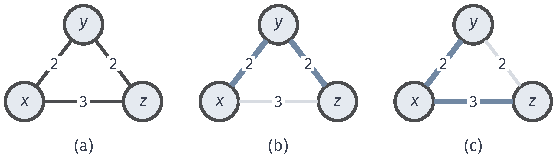
\includegraphics[width=95.793mm]{figures/01-basic-mathematics/04-graphs/tikz/c3-mst-vs-spt/figure.pdf}
  \caption{最小生成树与最短路树可以不同。(a) 原图，边旁为权。(b) 最小生成树$\{xy,yz\}$总成本$4$，但树上$x$到$z$的路线长$4$。(c) 以$x$为源的最短路树$\{xy,xz\}$保证每个顶点到$x$的距离最短，总成本却是$5$。蓝色粗边为所选的边。}
  \label{fig:graph-opt-mst-vs-spt}
\end{figure}

\paragraph{非连通、负权与平局}
图不连通时不存在生成树，问题改为在每个连通分量内分别求最小生成树，合起来称为\term{最小生成森林}（minimum spanning forest）。

负权不会带来最短路那样的困难：每棵生成树恰有$n-1$条边，把所有边权同时加上常数$c$，每棵生成树的成本都增加$(n-1)c$，比较结果不变，因此总可以设想权都为正。边权有相同值时，最小生成树可能不止一棵，但最小总成本是唯一的。

若要最大化总权，把全部边权取负即化为最小化问题，得到\term{最大生成树}（maximum spanning tree），下面的割性质与两种算法只需把“最小”改为“最大”即可照用。第~\ref{chap:general-graph-dp-construction}章构造团树时会用到最大生成树。

\section{割性质与安全选边}
\label{sec:graph-opt-cut-property}

两种算法都是逐条选边，并希望每一步都不走错。“不走错”的确切含义是：当前已选的边集$A$总能扩充成某一棵最小生成树。只要保持这个不变量，选满$n-1$条边时，$A$本身就是一棵最小生成树。问题在于，下一条边选哪条才能保持不变量。

回答这个问题要用到割。把顶点集分成两个非空部分$S$与$V\setminus S$，称为图的一个\term{割}（cut），记作$(S,V\setminus S)$。一条边的两个端点分别在两侧时，称它跨越这个割。若已选边集$A$中没有边跨越该割，就称这个割与$A$相容。跨越某个割的边中权最小的称为该割的\term{轻边}（light edge），权相同时轻边可以不止一条。与当前选边相容的任何一个割上，轻边都可以放心选入。

\begin{lemma}[割性质]
\label{lem:graph-opt-cut-property}
设$\mathcal G$是有限无向连通加权图，边集$A$包含在某棵最小生成树中，割$(S,V\setminus S)$与$A$相容，$e$是该割的一条轻边。则$A\cup\{e\}$也包含在某棵最小生成树中。
\end{lemma}

\begin{proof}
取一棵包含$A$的最小生成树$T$。若$e\in T$，结论已成立。否则把$e$加入$T$，由第~\ref{sec:graph-trees-forests}节，树加一条边恰好形成一个环。设$e=\{u,v\}$，$u\in S$、$v\notin S$，这个环由$e$与$T$中$u$到$v$的路径组成。这条路径从$S$出发，最终到达$V\setminus S$，所以其中至少有一条边$f$跨越该割。

从$T+e$中删去$f$，环被打断，所得边集$T'=T+e-f$仍连通且有$n-1$条边，因而是生成树。由于$e$是轻边，$w_e\leq w_f$，所以
\[
  w(T')=w(T)+w_e-w_f\leq w(T),
\]
$T'$也是最小生成树。最后，割与$A$相容，跨越割的$f$不在$A$中，删去$f$不影响$A$；于是$A\cup\{e\}\subseteq T'$。
\end{proof}

图~\ref{fig:graph-opt-cut-exchange}画出这一交换：轻边$e$加入后与树中路径形成环，环上另一条跨割边$f$被删去，成本不增。

\begin{figure}[!htb]
  \centering
  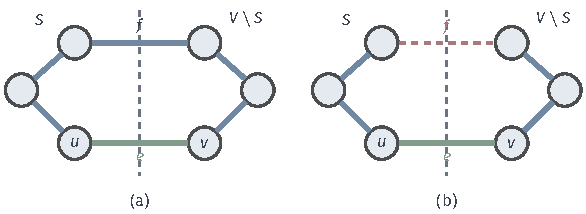
\includegraphics[width=99.187mm]{figures/01-basic-mathematics/04-graphs/tikz/c3-cut-exchange/figure.pdf}
  \caption{割性质的交换论证。虚线把顶点分成$S$与$V\setminus S$，蓝色粗边为最优树$T$，其中不跨割的边包含当前选边$A$。(a) 轻边$e$（绿色）不在$T$中，加入后与$T$中$u$到$v$的路径形成环。(b) 环上另一条跨割边$f$（红色虚线）被删去，得到$T'=T+e-f$，因$w_e\leq w_f$，成本不增。}
  \label{fig:graph-opt-cut-exchange}
\end{figure}

安全不等于必选。割性质只保证轻边能留在\emph{某一棵}最优树中，并不保证它出现在\emph{每一棵}最优树中。设三角形三条边的权都是$1$，取割$(\{x\},\{y,z\})$，$xy$与$xz$都是轻边。最小生成树$\{xy,yz\}$不含$xz$，但按割性质选入$xz$仍然安全，因为$\{xz,yz\}$同样是最小生成树。平局时不同的选择通向不同的最优树，最优成本却相同。

两种算法的区别只在于选取哪个割：Kruskal算法以当前森林中某个分量作为$S$，Prim算法以当前唯一一棵树的顶点集作为$S$。两者的正确性证明都归结为说明：被选入的边确实是所取割的轻边。

\section{Kruskal算法}
\label{sec:graph-opt-kruskal}

\subsection{问题与思路}

一种自然的想法是从最便宜的边开始逐条考虑，只要不形成环就选入。开始时每个顶点自成一个分量；一条边的两端若属于不同分量，选入它会把两个分量连起来，不会成环；若两端已在同一分量，选入它就会成环，应当跳过。每选一条边，分量数减一且不产生环，所以选边数加分量数始终等于$n$。判断两端是否同属一个分量，正是第~\ref{sec:graph-trav-union-find}小节并查集的用途。

\subsection{算法实现}

按权排好序的边序列预先构造，运行中不变。算法维护两项状态：
\begin{itemize}
  \item 已选边集$A$：初值为空；
  \item 并查集：其中的集合就是森林$(V,A)$的分量，初始时每个顶点自成一个集合。
\end{itemize}
按排序依次取边$\{u,v\}$，比较$\operatorname{find}(u)$与$\operatorname{find}(v)$：
\begin{itemize}
  \item 代表不同：把这条边加入$A$，执行$\operatorname{union}(u,v)$；
  \item 代表相同：选入会成环，跳过。
\end{itemize}
选满$n-1$条边时可提前停止，否则扫完全部边。

\begin{algorithm}[Kruskal算法]
\label{alg:graph-opt-kruskal}
输入：有限无向加权图。输出：最小生成森林的边集$A$。
\begin{enumerate}
  \item 把全部边按权从小到大排序，平局按固定的边序；令$A=\varnothing$，为每个顶点建立一个单元素集合。
  \item 按排序依次取边$\{u,v\}$：若$u,v$的代表不同，把这条边加入$A$并合并两个集合；若代表相同，跳过。
  \item 选满$n-1$条边时可提前停止；否则扫描完全部边，输出的$A$是最小生成森林，集合个数即连通分量数。
\end{enumerate}
\end{algorithm}

\paragraph{执行过程}
下面用一张五点七边图逐步演示。顶点为$a,b,c,d,e$，七条边已按权排好序：
\[
  \begin{gathered}
    w_{ab}=1,\quad w_{bc}=2,\quad w_{cd}=3,\quad w_{ac}=4,\\
    w_{bd}=5,\quad w_{ce}=6,\quad w_{de}=7.
  \end{gathered}
\]
表~\ref{tab:graph-opt-kruskal-trace}逐边列出判断与分量的变化，图~\ref{fig:graph-opt-kruskal-steps}画出了这一过程。

$ab$、$bc$、$cd$的两端都属于不同分量，依次选入，此时分量为$\{a,b,c,d\}$与$\{e\}$，累计成本$6$。

$ac$与$bd$的两端都已在$\{a,b,c,d\}$中，选入会成环，跳过。

$ce$连接两个分量，选入后只剩一个分量，已选满$4=n-1$条边，停止，$de$不必再检查。结果为$\{ab,bc,cd,ce\}$，总成本为
\[
  w_{ab}+w_{bc}+w_{cd}+w_{ce}=1+2+3+6=12.
\]

\begin{table}[!htb]
  \centering
  \caption{Kruskal算法在五点七边图上的状态变化。“两端分量”指处理该边之前两个端点所在的并查集集合；选满$4$条边后停止，$de$未被检查。}
  \label{tab:graph-opt-kruskal-trace}
  \begin{tabular}{@{}cccll@{}}
    \toprule
    边 & 权 & 两端分量 & 动作 & 处理后的分量与累计成本 \\
    \midrule
    $ab$ & $1$ & $\{a\}$，$\{b\}$ & 选入 & $\{a,b\},\{c\},\{d\},\{e\}$；$1$ \\
    $bc$ & $2$ & $\{a,b\}$，$\{c\}$ & 选入 & $\{a,b,c\},\{d\},\{e\}$；$3$ \\
    $cd$ & $3$ & $\{a,b,c\}$，$\{d\}$ & 选入 & $\{a,b,c,d\},\{e\}$；$6$ \\
    $ac$ & $4$ & 同为$\{a,b,c,d\}$ & 跳过 & 不变；$6$ \\
    $bd$ & $5$ & 同为$\{a,b,c,d\}$ & 跳过 & 不变；$6$ \\
    $ce$ & $6$ & $\{a,b,c,d\}$，$\{e\}$ & 选入 & $\{a,b,c,d,e\}$；$12$ \\
    \bottomrule
  \end{tabular}
\end{table}

\begin{figure}[!htb]
  \centering
  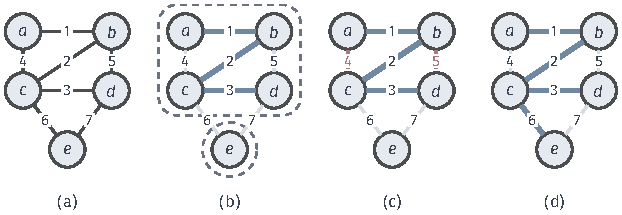
\includegraphics[width=106.5mm]{figures/01-basic-mathematics/04-graphs/tikz/c3-kruskal-steps/figure.pdf}
  \caption{Kruskal算法在五点七边图上的过程。(a) 原图，边旁为权。(b) 依次选入$ab,bc,cd$（蓝色粗边），虚线框标出当前分量$\{a,b,c,d\}$与$\{e\}$。(c) $ac$与$bd$的两端已在同一分量，选入会成环，跳过（红色虚线）。(d) 选入$ce$，得到最小生成树$\{ab,bc,cd,ce\}$，总成本$12$。}
  \label{fig:graph-opt-kruskal-steps}
\end{figure}

\subsection{算法分析}

\paragraph{正确性}
选入的边是否安全，由割性质判断。

\begin{theorem}[Kruskal算法的正确性]
\label{thm:graph-opt-kruskal}
对有限无向加权图，算法~\ref{alg:graph-opt-kruskal}输出一个最小生成森林；图连通时输出最小生成树。
\end{theorem}

\begin{proof}
先设图连通，证明不变量“$A$包含在某棵最小生成树中”。初始$A=\varnothing$，结论成立。设算法即将选入边$e=\{u,v\}$，取$S$为森林$(V,A)$中$u$所在的分量，则$v\notin S$，割$(S,V\setminus S)$与$A$相容。

考察任意一条跨越这个割、权小于$w_e$的边$g$。它排在$e$之前，已被处理过：若当时被选入，它就在$A$中，而$A$中没有跨割的边；若当时被跳过，它的两端当时已在同一分量，分量只会合并而不会拆开，现在仍在同一分量，也不能跨割。所以跨越该割的边权都不小于$w_e$，$e$是轻边，由引理~\ref{lem:graph-opt-cut-property}，选入$e$后不变量仍成立。

扫描结束时，若原图中某条边连接了$(V,A)$的两个不同分量，处理到它时两端必属不同分量，它就会被选入，矛盾。所以$(V,A)$的分量与原图的分量相同，图连通时$A$是生成树。它包含在某棵最小生成树中，又与之边数相同，因而本身就是最小生成树。图不连通时，对每个分量分别应用上面的论证，结论对最小生成森林同样成立。
\end{proof}

\paragraph{复杂度}
排序需要$O(m\log m)$时间。之后至多处理$m$条边，每条边做两次$\operatorname{find}$，选入时再做一次$\operatorname{union}$，共$O(m)$次并查集操作。只用按大小合并时，由定理~\ref{thm:graph-trav-union-by-size}，每次操作$O(\log n)$，这部分为$O(m\log n)$；由于$m\leq n^2$，$\log m\leq2\log n$，总时间为$O(m\log n)$，空间为边表与并查集的$O(n+m)$。若再配合路径压缩，并查集操作的摊还开销几乎为常数，此时排序成为主要开销。算法的正确性只依赖割性质，与并查集采用哪种实现无关。

\section{Prim算法}
\label{sec:graph-opt-prim}

\subsection{问题与思路}

Kruskal算法同时维护许多分量。另一种做法是只让一棵树生长：从一个顶点出发，每次把一个外部顶点用最便宜的边接到树上。这时取的割就是“树内与树外”，只要能随时知道每个外部顶点离树最近的那条边，就能找到这个割的轻边。

\subsection{算法实现}

输入是图的邻接表与起点$r$。算法维护三项状态：
\begin{itemize}
  \item 树的顶点集$S$：初值为$\{r\}$；
  \item 键$\operatorname{key}(v)$与父点$p(v)$：外部顶点$v$与当前树之间最便宜的边的权及这条边在树内的端点，初始时$r$的邻居$v$取$w_{r,v}$与$r$，其余键为$+\infty$。键是\emph{一条}连接边的权，不是Dijkstra算法中的累计长度；
  \item 优先队列：按键存放外部顶点，支持取最小与降键，实现与第~\ref{sec:graph-opt-dijkstra}节相同。
\end{itemize}
当$S\neq V$时，每一轮做两件事：
\begin{itemize}
  \item 取出：把键最小的外部顶点$u$移出队列并加入$S$，把边$\{p(u),u\}$加入树；
  \item 更新：对$u$的每个外部邻居$v$，若$w_{u,v}<\operatorname{key}(v)$，令$\operatorname{key}(v)=w_{u,v}$、$p(v)=u$，并在队列中降键。
\end{itemize}
$S=V$时停止。

\begin{algorithm}[Prim算法]
\label{alg:graph-opt-prim}
输入：有限无向连通加权图、起点$r$。输出：最小生成树的边集。
\begin{enumerate}
  \item 令$S=\{r\}$；对$r$的每个邻居$v$，令$\operatorname{key}(v)=w_{r,v}$、$p(v)=r$，其余外部顶点的键为$+\infty$。
  \item 当$S\neq V$时，取出键最小的外部顶点$u$，把$u$加入$S$，把边$\{p(u),u\}$加入树。
  \item 对$u$的每个外部邻居$v$，若$w_{u,v}<\operatorname{key}(v)$，令$\operatorname{key}(v)=w_{u,v}$、$p(v)=u$。
\end{enumerate}
\end{algorithm}

\paragraph{执行过程}
在与Kruskal算法相同的五点图上从$a$出发，各步状态见表~\ref{tab:graph-opt-prim-trace}与图~\ref{fig:graph-opt-prim-steps}。开始时$\operatorname{key}(b)=1$、$\operatorname{key}(c)=4$。

取出$b$，选入$ab$；$b$的邻边把$c$的键从$4$改为$2$，并给$d$设键$5$。

取出$c$，选入$bc$；$d$的键从$5$改为$3$，$e$得到键$6$。

取出$d$，选入$cd$；$de=7$不优于$e$现有的键$6$，不更新。

最后取出$e$，选入$ce$。所得的树与Kruskal算法相同，成本$12$。

\begin{table}[!htb]
  \centering
  \caption{Prim算法从$a$出发的状态。每行是取出一个顶点并更新键之后的情形，括号内为键对应的父点，“—”表示该顶点已入树。}
  \label{tab:graph-opt-prim-trace}
  \begin{tabular}{@{}cccccc@{}}
    \toprule
    取出 & 选入的边 & $\operatorname{key}(b)$ & $\operatorname{key}(c)$ & $\operatorname{key}(d)$ & $\operatorname{key}(e)$ \\
    \midrule
    初始（$S=\{a\}$） & — & $1$（$a$） & $4$（$a$） & $+\infty$ & $+\infty$ \\
    $b$ & $ab$ & — & $2$（$b$） & $5$（$b$） & $+\infty$ \\
    $c$ & $bc$ & — & — & $3$（$c$） & $6$（$c$） \\
    $d$ & $cd$ & — & — & — & $6$（$c$） \\
    $e$ & $ce$ & — & — & — & — \\
    \bottomrule
  \end{tabular}
\end{table}

\begin{figure*}[!htb]
  \centering
  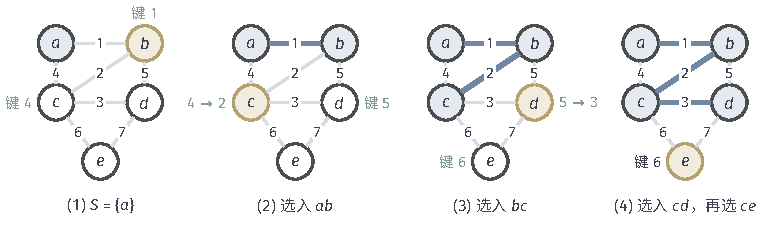
\includegraphics[width=129.858mm]{figures/01-basic-mathematics/04-graphs/tikz/c3-prim-steps/figure.pdf}
  \caption{Prim算法从$a$出发的过程。每个面板中蓝色顶点与蓝色粗边是当前树，外部顶点旁标出键，绿色表示刚被改善的键，黄色为下一个取出的顶点。依次选入$ab,bc,cd,ce$，各步加入的边恰是当前树顶点集所形成割的轻边；最终的树与Kruskal算法相同，成本$12$。}
  \label{fig:graph-opt-prim-steps}
\end{figure*}

换一个起点，选边次序会变。从$e$出发时，$c$与$d$的键分别为$6$与$7$；先选入$ec=6$，$c$的邻边使$b$、$a$、$d$的键变为$2$、$4$、$3$；再选入$cb=2$，$a$的键降为$1$；随后选入$ba=1$与$cd=3$。

这次所选边权依次为$6,2,1,3$，并不递增。这与Kruskal算法的全局排序不同：Prim算法每次只在当前割上取最轻的边，不同时刻面对的是不同的割。

\subsection{算法分析}

\paragraph{正确性}
每个外部顶点的键始终等于它与$S$之间最便宜的边权：初始时成立；$u$入树后，新增的跨割边只有从$u$出发的那些，更新一步恰好逐一比较它们。于是取出的最小键对应割$(S,V\setminus S)$的一条轻边。令$A$为当前树的边集，$A$的边都在$S$内部，割与$A$相容；由引理~\ref{lem:graph-opt-cut-property}，若$A$包含在某棵最小生成树中，加入新边后仍然如此。从$A=\varnothing$出发归纳，选满$n-1$条边时得到最小生成树。

\paragraph{复杂度}
用数组保存键、每次线性扫描找最小时，$n$次取最小共$O(n^2)$，每条边至多引起一次键的比较与更新，总时间为$O(n^2+m)$，适合稠密图。用支持降键的索引二叉堆时，取最小与降键各需$O(\log n)$，总时间为$O((n+m)\log n)$，适合稀疏图。两种实现的额外空间都是$O(n)$。

\paragraph{非连通情形}
图不连通时，一棵树长满所在分量后，外部顶点的键全为$+\infty$，这时从任一尚未访问的顶点重新开始，得到最小生成森林，各分量的父边与成本分别保留。

\section{方法比较与结果检验}
\label{sec:graph-opt-mst-comparison}

两种算法读取边与维护状态的方式不同。Kruskal算法对全部边排序，按全局次序检查，用并查集维护多个分量，适合边以列表给出的稀疏图。Prim算法只读取新入树顶点的邻边，用键数组或堆维护局部信息；在邻接矩阵存储的稠密图上，数组版本的$O(n^2)$开销与读入图同阶。孰优孰劣取决于图的稠密程度、边的组织方式和所用数据结构，不能只凭算法名称判断。

检验一份声称的最小生成森林时，先确认它是一个可行的生成森林：所选的每条边都来自原图；每个原连通分量的顶点都被覆盖；所选边无环，可以用并查集逐条加入核对；选边数等于$n$减去分量数。然后重算总成本。这些检查只证明结果是\emph{一个}生成森林，不能证明它最优。

最优性另有一份不依赖算法过程的判据。对每条未被选中的边$\{u,v\}$，考察树上$u$到$v$的唯一路径。若路径上有一条边的权大于$w_{u,v}$，用这条非树边替换它，就得到成本更低的生成树，结果必不最优。反过来，没有这样的边也足以保证最优。

\begin{theorem}[非树边条件]
\label{thm:graph-opt-mst-cycle-certificate}
设$T$是有限无向连通加权图的一棵生成树。若对每条非树边$f=\{u,v\}$，$T$中$u$到$v$路径上的每条边$g$都满足$w_g\leq w_f$，则$T$是最小生成树。
\end{theorem}

\begin{proof}
在全部最小生成树中取一棵与$T$公共边最多的$T^\star$。若$T^\star=T$，结论成立。否则取$f\in T^\star\setminus T$。从$T^\star$中删去$f$，顶点分成两块，$f$是$T^\star$中唯一跨越这两块的边。$f$不在$T$中，是$T$的非树边，$T$中连接$f$两端的路径从一块出发到达另一块，必含一条跨越两块的边$g$；$g\neq f$，所以$g\notin T^\star$。由条件$w_g\leq w_f$，$T^\star-f+g$仍是生成树，成本不超过$w(T^\star)$，因而也是最小生成树，而它与$T$的公共边比$T^\star$多一条，与$T^\star$的取法矛盾。
\end{proof}

在五点图上核对。三条非树边在树上各对应一条路径，路径边权如下：
\[
  \begin{aligned}
    ac=4&:\quad a\text{--}b\text{--}c,\ \text{边权}\ 1,2;\\
    bd=5&:\quad b\text{--}c\text{--}d,\ \text{边权}\ 2,3;\\
    de=7&:\quad d\text{--}c\text{--}e,\ \text{边权}\ 3,6.
  \end{aligned}
\]
每条非树边都不轻于对应路径上的边，所以$\{ab,bc,cd,ce\}$最优。这一检查对每条非树边沿树找一次路径，朴素实现为$O(nm)$。

小规模的例子还可以枚举全部生成树作对照：这个图共有$21$棵生成树，成本$12$的只有上面这一棵，次优的成本为$13$。但两种算法在某个例子上给出相同的树，只是一致性的旁证，不能当作一般正确性的证明。

\FloatBarrier
\section{本章小结}
\label{sec:mst-summary}

章首的问题是：能否逐条选边，只看局部就断定没有选错。割性质给出肯定的回答：若已选边集包含在某棵最小生成树中，那么在任何与它相容的割上，选入一条轻边后仍包含在某棵最小生成树中。证明靠交换论证，即加入轻边、删去环上另一条跨割边，成本不增。安全不等于必选：权相同时轻边可能有多条，不同选择通向不同的最优树，最优成本却相同。

两种算法只是选取的割不同。Kruskal算法按全局边权次序检查，以当前森林的一个分量为割的一侧，用并查集判断成环，总时间为$O(m\log n)$，配合路径压缩时主要开销是排序；它自然地给出不连通图的最小生成森林。Prim算法只让一棵树生长，以树内与树外为割，键记录每个外部顶点的最便宜接入边。数组实现为$O(n^2+m)$，适合稠密图；二叉堆实现为$O((n+m)\log n)$，适合稀疏图。

最小生成树最小化的是整组边的总造价，不是两点间路线的长度，树上两点间的路径未必是最短路，键也不同于Dijkstra算法的累计距离。负权不造成困难，因为每棵生成树的边数都是$n-1$，所有边权同加一个常数不改变比较结果。结果的检验分两步：先核对所选边构成生成森林，再核对每条非树边都不轻于它在树上所对应路径中的边，后者足以保证最优。

把选边次序改为从大到小，同样的论证就求出最大生成树；第~\ref{chap:general-graph-dp-construction}章以团的交集大小为边权构造团树时，调用的正是它。下一章转向另一种选择对象：不再挑出一组边，而是给每条弧分配一个流量。

% 第5章：最大流与最小割（流、容量与割；残量网络与增广；Edmonds--Karp算法；Dinic算法；方法比较与结果检验）。

\chapter{最大流与最小割}
\label{sec:graph-max-flow}
\label{chap:max-flow-min-cut}

前两章各选出一个结构：一条路线或一棵树。现在设想从水厂向用户输水，每段管道有输送上限，水可以并行、汇合、分流，问单位时间内最多能送出多少水。这次选择的对象是每条弧上的流量，它们要同时满足容量上限和中途不积存的条件。本章要回答两个问题：怎样逐步改进一个输送方案，以及怎样确认一个方案已经不能再改进。

第~\ref{sec:graph-opt-flow-cut}节先给出上界：任何一组把源与汇隔开的管道，其容量之和都限制了输送量，这组管道称为割。第~\ref{sec:graph-opt-residual-network}节处理改进：先选的路线可能占用别的路线需要的容量，所以要允许把已送出的流量改道。记录“还能追加多少、能撤回多少”的残量网络把改进统一为找一条增广路径，找不到时恰好能读出一个与流值相等的割，这就是最大流最小割定理的内容。

具体算法的差别在于怎样找路。第~\ref{sec:graph-opt-edmonds-karp}节的Edmonds--Karp算法每次用广度优先遍历找一条弧数最少的路，增广次数因此与容量数值无关；第~\ref{sec:graph-opt-dinic}节的Dinic算法一次分层后在层内把能走的最短路都堵住，再重建层次。第~\ref{sec:graph-opt-max-flow-analysis}节比较两者，并说明怎样用流与割核对结果。本章记顶点数为$n$、原弧数为$a$，残量网络沿用第~\ref{sec:graph-bfs}节的广度优先遍历与邻接表。

\section{流、容量与割}
\label{sec:graph-opt-flow-cut}

设$\mathcal G=(V,E)$是有限有向图，指定两个不同的顶点：源点$s$与汇点$t$。每条弧$u\to v$带有有限非负实数\emph{容量}$c_{u,v}$，表示该弧单位时间内最多能通过的量。这样的四元组$(\mathcal G,c,s,t)$称为\term{流网络}（flow network）。

\begin{definition}[流与流值]
\label{def:graph-opt-flow}
流网络上的一个\term{流}（flow）是给每条弧$u\to v$赋予实数$x_{u,v}$的一组数$\bm x=(x_{u,v})$，满足
\begin{gather}
  0\leq x_{u,v}\leq c_{u,v}\quad\text{对每条弧}\ u\to v,\label{eq:graph-opt-capacity}\\
  \sum_{u:\,u\to v}x_{u,v}=\sum_{w:\,v\to w}x_{v,w}\quad\text{对每个}\ v\in V\setminus\{s,t\}.\label{eq:graph-opt-conservation}
\end{gather}
前者称为容量约束，后者称为\term{流守恒}（flow conservation）。源点的净流出
\begin{equation}
  \operatorname{val}(\bm x)=\sum_{w:\,s\to w}x_{s,w}-\sum_{u:\,u\to s}x_{u,s}
  \label{eq:graph-opt-flow-value}
\end{equation}
称为\term{流值}（flow value）。流值最大的流称为\term{最大流}（maximum flow）。
\end{definition}

中间顶点只转运、不积存。把各顶点的净流出（流出减流入）全部相加，每条弧的流量一正一负，总和为零；中间顶点的净流出都是零，于是源点的净流出等于汇点的净流入，$\operatorname{val}(\bm x)$也是$t$收到的净量。流值不是全图各弧流量的总和：一单位流量经过三条弧到达汇点，只算一单位流值。

为了估计流值能有多大，把顶点分成包含$s$的一侧$S$与包含$t$的一侧$\bar S=V\setminus S$，称$(S,\bar S)$为一个$s$--$t$割。这沿用第~\ref{sec:graph-opt-cut-property}节割的含义，只是要求源、汇分居两侧。割的\term{割容量}（cut capacity）只累计从源侧跨向汇侧的弧：
\begin{equation}
  c(S,\bar S)=\sum_{u\in S,\ v\in\bar S,\ u\to v}c_{u,v}.
  \label{eq:graph-opt-cut-capacity}
\end{equation}
从汇侧指回的弧不计入。直观上，从$s$到$t$的输送都要穿过这个割，总量不能超过这些弧的容量之和。

\begin{lemma}[流值不超过割容量]
\label{lem:graph-opt-weak-duality}
对任意流$\bm x$与任意$s$--$t$割$(S,\bar S)$，有
\begin{equation}
  \operatorname{val}(\bm x)=\sum_{u\in S,\,v\in\bar S}x_{u,v}-\sum_{v\in\bar S,\,u\in S}x_{v,u}\leq c(S,\bar S).
  \label{eq:graph-opt-net-flow-cut}
\end{equation}
\end{lemma}

\begin{proof}
对$S$中的全部顶点把净流出相加。$s$贡献$\operatorname{val}(\bm x)$，其余顶点都是中间顶点（$t\notin S$），贡献为零，所以和等于$\operatorname{val}(\bm x)$。另一方面，两端都在$S$内的弧在起点计正、在终点计负，相互抵消；剩下的只有跨割的弧：从$S$指向$\bar S$的弧计正，从$\bar S$指回$S$的弧计负。这就得到式~\eqref{eq:graph-opt-net-flow-cut}中的等式。再由容量约束，第一个和不超过$c(S,\bar S)$，第二个和不小于零，得到不等式。
\end{proof}

图~\ref{fig:graph-flow-cut-cancellation}把抵消发生的位置画出来：内部弧$s\to u$在两端各出现一次且符号相反，真正留在总和里的只有跨界的$b,c,d$。

\begin{figure}[!htb]
  \centering
  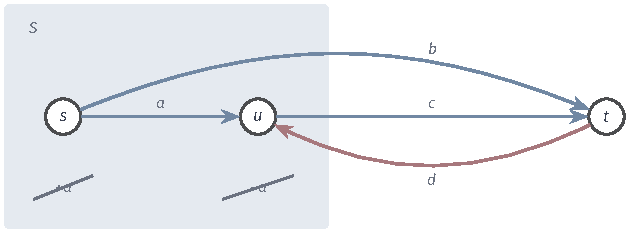
\includegraphics[width=106.535mm]{figures/03-graphs/02-combinatorial-optimization/tikz/flow-cut-cancellation/figure.pdf}
  \caption{对源侧顶点的净流出求和。浅蓝区域为$S=\{s,u\}$，弧旁字母表示流量。内部弧的$a$与$-a$相抵；跨出弧$b,c$计正，指回弧$d$计负，所以总和为$b+c-d$。若$u$满足守恒，该总和恰等于源点的净流出。}
  \label{fig:graph-flow-cut-cancellation}
\end{figure}

于是流值等于跨过任意一个割的净流量，每个割的容量都是流值的上界。若某个流与某个割数值相等，这个流就不可能再增大，这个割也不可能更小。图~\ref{fig:graph-opt-flow-network-cut}给出一例：取$S=\{s,b\}$，净流量$3+3-1=5$恰为流值，不超过割容量$6$。

\begin{figure}[!htb]
  \centering
  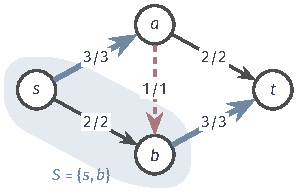
\includegraphics[width=50.295mm]{figures/01-basic-mathematics/04-graphs/tikz/c3-flow-network-cut/figure.pdf}
  \caption{流网络、流与割。弧旁“$x/c$”为流量与容量，流值为$5$。浅色底为源侧$S=\{s,b\}$：跨出弧$s\to a$、$b\to t$（蓝色粗弧）计入割容量$3+3=6$；指回弧$a\to b$（红色虚线）不计容量，其流量从净流量中扣除。}
  \label{fig:graph-opt-flow-network-cut}
\end{figure}

\section{残量网络与增广}
\label{sec:graph-opt-residual-network}

候选的流有无穷多个，只能从一个可行流出发逐步改进。最朴素的办法是找一条每条弧都有空余的$s$--$t$路径多送一些，但先选的路线可能占用别的路线需要的容量。

下面的单位容量网络说明这一点：弧$s\to a$、$s\to b$、$a\to b$、$a\to t$、$b\to t$的容量都为$1$。若先沿$s\to a\to b\to t$送一单位，三条弧都满了，剩下的$s\to b$与$a\to t$连不成路径，只会追加的办法停在流值$1$；而$s\to a\to t$与$s\to b\to t$本可送出$2$。

补救的办法是允许撤回旧流量，把撤回也当作一种可走的“通道”。给定流$\bm x$，对每条原弧$u\to v$建立两条\emph{残量弧}：正向残量弧$u\to v$，容量$c_{u,v}-x_{u,v}$，表示还能追加多少；反向残量弧$v\to u$，容量$x_{u,v}$，表示能撤回多少。只保留容量为正的残量弧，得到的有向图称为\term{残量网络}（residual network），记作$\mathcal G_{\bm x}$，残量弧的容量记作$r_{\bm x}$。

例如原弧容量为$3$、当前流量为$2$时，正向残量为$1$、反向残量为$2$（图~\ref{fig:graph-opt-residual-arc}）：沿$u\to v$再送$1$表示追加，沿$v\to u$送$2$表示把原弧上的流量全部撤回，并不要求原网络中真有一条从$v$到$u$的管道。

\begin{figure}[!htb]
  \centering
  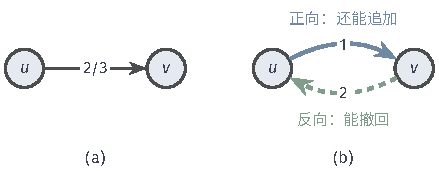
\includegraphics[width=74.186mm]{figures/01-basic-mathematics/04-graphs/tikz/c3-residual-arc/figure.pdf}
  \caption{一条原弧对应两条残量弧。(a) 原弧$u\to v$容量$3$、流量$2$。(b) 正向残量弧（蓝色）容量$1$，可追加；反向残量弧（绿色虚线）容量$2$，可撤回。流量为$0$时无反向弧，满流时无正向弧。}
  \label{fig:graph-opt-residual-arc}
\end{figure}

回到单位容量的例子。第一次送流后，残量网络中出现反向残量弧$b\to a$，于是有路径$s\to b\to a\to t$：在$s\to b$与$a\to t$上各追加一单位，同时把$a\to b$上的流量撤回一单位。更新后$a\to b$为$0$，其余四条弧各为$1$，流值为$2$（图~\ref{fig:graph-opt-undo-flow}）：第一次经过$a\to b$的那一单位被“改道”到了$a\to t$。

\begin{figure*}[!htb]
  \centering
  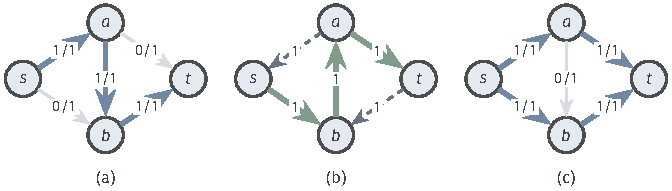
\includegraphics[width=113.686mm]{figures/01-basic-mathematics/04-graphs/tikz/c3-undo-flow/figure.pdf}
  \caption{单位容量网络中撤回旧流量。(a) 沿$s\to a\to b\to t$送一单位（蓝色粗弧）后，只用正向残量已无$s$--$t$路径。(b) 残量网络中绿色路径$s\to b\to a\to t$经过反向残量弧$b\to a$（灰色为其余反向弧）。(c) 更新后$a\to b$的流量被撤回，流值为$2$。}
  \label{fig:graph-opt-undo-flow}
\end{figure*}

有了反向残量弧，改进一个流就统一成了找路。残量网络$\mathcal G_{\bm x}$中从$s$到$t$的简单路径$P$称为关于$\bm x$的\term{增广路径}（augmenting path）。$P$上残量容量的最小值
\begin{equation}
  \Delta=\min_{(u\to v)\in P}r_{\bm x}(u,v)>0
  \label{eq:graph-opt-bottleneck}
\end{equation}
称为$P$的\term{瓶颈容量}（bottleneck capacity），即这条路一次最多能多送的量。

沿$P$增广$\Delta$，是指对$P$上的每条残量弧：若它是原弧$u\to v$的正向残量，令$x_{u,v}\leftarrow x_{u,v}+\Delta$；若它是原弧$v\to u$的反向残量，令$x_{v,u}\leftarrow x_{v,u}-\Delta$。

\begin{lemma}[沿增广路径更新保持可行]
\label{lem:graph-opt-augment}
设$\bm x$是流，$P$是增广路径，瓶颈容量为$\Delta$。沿$P$增广$\Delta$后得到的$\bm x'$仍是流，并且$\operatorname{val}(\bm x')=\operatorname{val}(\bm x)+\Delta$。
\end{lemma}

\begin{proof}
容量约束：正向残量弧满足$\Delta\leq c_{u,v}-x_{u,v}$，追加后不超过容量；反向残量弧满足$\Delta\leq x_{v,u}$，撤回后不小于零。

流守恒：$P$经过每个中间顶点$v$恰好一次，一条残量弧进入$v$，一条离开$v$。进入的那条若是正向残量，$v$的流入增加$\Delta$；若是反向残量，即撤回一条从$v$出发的原弧上的流量，$v$的流出减少$\Delta$。两种情形都使$v$的净流出减少$\Delta$。同理，离开的那条使$v$的净流出增加$\Delta$，两者相抵。

最后，$P$的第一条残量弧离开$s$，使$s$的净流出增加$\Delta$，而$P$不再回到$s$，所以流值增加$\Delta$。
\end{proof}

引理直接给出一个改进框架：从零流出发，只要残量网络中还有增广路径就沿它增广。这个框架称为\term{Ford--Fulkerson方法}（Ford--Fulkerson method）。称它为“方法”，是因为它没有规定选哪条路，后面两种算法给出不同的规定。

\begin{algorithm}[Ford--Fulkerson增广框架]
\label{alg:graph-opt-ford-fulkerson}
输入：流网络$(\mathcal G,c,s,t)$。输出：流$\bm x$与割$(S,\bar S)$。
\begin{enumerate}
  \item 令$\bm x=\bm 0$。
  \item 在$\mathcal G_{\bm x}$中从$s$搜索；若到达不了$t$，令$S$为搜索到的顶点集，输出$\bm x$与$(S,\bar S)$，停止。
  \item 取一条增广路径$P$，求瓶颈$\Delta$，按引理~\ref{lem:graph-opt-augment}更新$\bm x$，回到第2步。
\end{enumerate}
\end{algorithm}

框架能否停下来，取决于每次能送多少。

\begin{theorem}[整数容量下的有限终止]
\label{thm:graph-opt-integer-termination}
若所有容量都是非负整数，则无论怎样选择增广路径，算法~\ref{alg:graph-opt-ford-fulkerson}至多经过$C_s=\sum_{w:\,s\to w}c_{s,w}$次增广就停止，并且全程每条弧上的流量都是整数。
\end{theorem}

\begin{proof}
零流是整数的；若当前流量都是整数，则残量$c_{u,v}-x_{u,v}$与$x_{u,v}$都是整数，瓶颈$\Delta$是正整数，更新后流量仍为整数。于是每次增广使流值至少增加$1$。另一方面，取$S=\{s\}$，由引理~\ref{lem:graph-opt-weak-duality}，流值不超过$C_s$，所以增广至多$C_s$次。
\end{proof}

容量为有理数时，乘以公分母即化为整数情形。对一般实容量，这个论证不能照搬：增加量可能越来越小。已知存在含无理容量的网络，任意选路的框架永不停止，流值甚至收敛到小于最大流值的数。

框架停止时没有增广路径。这时的流是最大的，而且可以从残量网络中直接读出一个与流值相等的割。

\begin{theorem}[增广路径判据]
\label{thm:graph-opt-augmenting-path}
设$\bm x$是流网络上的一个流，则下列三条等价：
\begin{enumerate}
  \item $\bm x$是最大流；
  \item 残量网络$\mathcal G_{\bm x}$中不存在增广路径；
  \item 存在某个$s$--$t$割$(S,\bar S)$，使$\operatorname{val}(\bm x)=c(S,\bar S)$。
\end{enumerate}
此时$(S,\bar S)$是割容量最小的$s$--$t$割，可取$S$为$\mathcal G_{\bm x}$中从$s$可达的顶点集。
\end{theorem}

\begin{proof}
由1推2：若存在增广路径，由引理~\ref{lem:graph-opt-augment}可得流值更大的流，与$\bm x$最大矛盾。

由2推3：令$S$为$\mathcal G_{\bm x}$中从$s$可达的顶点集。$s\in S$，而没有增广路径说明$t\notin S$。若$u\in S$、$v\in\bar S$且$u\to v$是原弧，则必有$x_{u,v}=c_{u,v}$，否则正向残量弧$u\to v$存在，$v$就从$s$可达了。若$v\in\bar S$、$u\in S$且$v\to u$是原弧，则必有$x_{v,u}=0$，否则反向残量弧$u\to v$存在，同样使$v$可达。代入式~\eqref{eq:graph-opt-net-flow-cut}，第一个和等于$c(S,\bar S)$，第二个和为零，故$\operatorname{val}(\bm x)=c(S,\bar S)$。

由3推1：对任意流$\bm y$，引理~\ref{lem:graph-opt-weak-duality}给出$\operatorname{val}(\bm y)\leq c(S,\bar S)=\operatorname{val}(\bm x)$，所以$\bm x$最大。同一不等式对任意割$(S',\bar S')$给出$c(S',\bar S')\geq\operatorname{val}(\bm x)=c(S,\bar S)$，所以$(S,\bar S)$的割容量最小。
\end{proof}

割容量最小的$s$--$t$割称为\term{最小割}（minimum cut）。定理把“是否最优”化成在残量网络中做一次遍历就能回答的问题；停止时的流与割互为证书，可以逐弧核对，不必相信算法过程。

结合定理~\ref{thm:graph-opt-integer-termination}，整数容量的网络存在每条弧流量都为整数的最大流，第~\ref{sec:graph-matching}节会用到这一点。图~\ref{fig:graph-opt-max-flow-certificate}是同一网络的最大流及其证书。需要注意，判据只检验给定的流；一般实容量下能否有限步到达这样的流，要由具体的选路规则保证。

\begin{figure}[!htb]
  \centering
  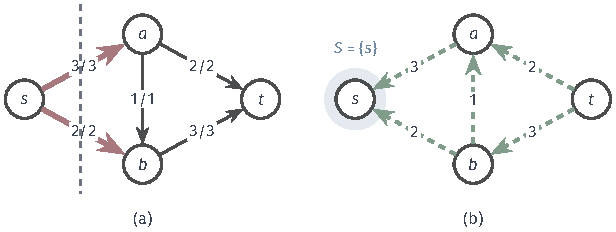
\includegraphics[width=104.186mm]{figures/01-basic-mathematics/04-graphs/tikz/c3-max-flow-certificate/figure.pdf}
  \caption{最大流与最小割互为证书。(a) 最大流，弧旁为“流量/容量”，流值为$5$；虚线为割$(\{s\},\{a,b,t\})$，跨出弧（红色）均满流，割容量$3+2=5$。(b) 残量网络只剩反向残量弧（绿色虚线），$s$没有出弧，可达集为$S=\{s\}$（浅色底）。}
  \label{fig:graph-opt-max-flow-certificate}
\end{figure}

实现时，后面两种算法共用同一种表示。每条原弧$u\to v$登记一对残量边，分别挂在$u$、$v$的邻接表上，互相指向对方。每条残量边$e$记录终点、当前残量$r_e$和同伴边$\bar e$的编号；正向边初值$r_e=c_{u,v}$，反向边初值为$0$。沿$e$送$\Delta$时令$r_e\gets r_e-\Delta$、$r_{\bar e}\gets r_{\bar e}+\Delta$，两条边总是成对更新，原弧流量随时可读作其反向边的残量。

真实的反向弧与平行弧各有自己的边对，“真实反向输送”与“撤回流量”不会混为一谈。因此搜索时要记住到达每个顶点所经的\emph{边编号}，只记前一个顶点无法确定改哪条边。

\section{Edmonds--Karp算法}
\label{sec:graph-opt-edmonds-karp}

Edmonds--Karp算法保留残量网络与增广更新，只规定每轮用广度优先遍历选出弧数最少的增广路径。这条规则决定了增广次数能否摆脱容量数值的影响。

\subsection{主要思想}

把$s$看作供水处、$t$看作收水处，$a,b$为中转点。下面用这样一个网络说明选路的影响：四条外弧$s\to a$、$s\to b$、$a\to t$、$b\to t$容量都为$4$，中间弧$a\to b$容量为$1$，最大流值为$8$。

先选$s\to a\to b\to t$，瓶颈是中间弧，只能送$1$；再选$s\to b\to a\to t$，经反向残量弧$b\to a$撤回那一单位，又只增加$1$。两步后中间弧恢复空闲，同样两条路可以再选。一直交替，送满$8$要增广$8$次（图~\ref{fig:graph-opt-edmonds-karp-choice}(a)）。若外弧容量改为$10^6$，就要$2\times10^6$次。

回到零流，一层一层看：一步到$a,b$，两步到$t$。这样首先找到两弧路$s\to a\to t$，送$4$；再找到$s\to b\to t$，又送$4$，两次就达到$8$（图~\ref{fig:graph-opt-edmonds-karp-choice}(b)）。

这就是\emph{最短增广路}规则：在残量网络中用广度优先遍历找弧数最少的$s$--$t$路径。遍历决定走哪条路，瓶颈决定这次送多少；路径长短只数弧的条数，容量不参与比较。

\begin{figure}[!htb]
  \centering
  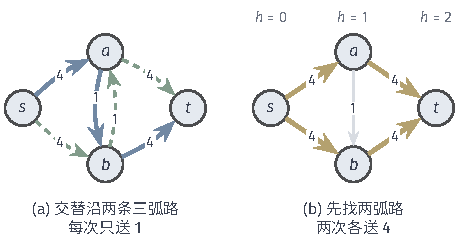
\includegraphics[width=78.444mm]{figures/01-basic-mathematics/04-graphs/tikz/c3-edmonds-karp-choice/figure.pdf}
  \caption{选路规则决定增广次数。外弧容量$4$，中间弧$a\to b$容量$1$。(a) 交替选蓝色路径$s\to a\to b\to t$与绿色虚线路径$s\to b\to a\to t$（经反向残量$b\to a$），每次送$1$，共$8$次。(b) 按层数$h$先找到两条两弧路径（黄色），两次各送$4$。}
  \label{fig:graph-opt-edmonds-karp-choice}
\end{figure}

一般情况下，弧数最少的路未必瓶颈最大；规则的保证来自另一处：增广不会让任何顶点离$s$更近，于是同一条弧不能频繁地成为瓶颈，这在后面证明。Sedgewick与Wayne的最大流实现正是用广度优先遍历选路\scite{math-graph-sedgewick-maxflow}。

\subsection{算法流程}

\paragraph{算法状态与初始化}
手工找路要记住：哪些管道还能追加或撤回、本轮找到了哪些点、各点经哪条边到达、共送出多少。残量边对的结构（邻接表、终点与同伴编号）建图后不变，不算状态。算法维护：
\begin{itemize}
  \item 残量$r_e$：每条残量边一个，正向边初值为容量，反向边初值为$0$，跨轮保留；
  \item 流值$F$：初值为$0$，跨轮累加；
  \item 访问标记与队列：每轮开始时清空，只标记$s$、队列只含$s$；
  \item 前驱边$\pi(v)$：到达$v$所经的残量边编号，每轮开始时清空。
\end{itemize}

\paragraph{一次增广与停止}
每一轮做三件事：
\begin{itemize}
  \item 搜索：按广度优先次序取出顶点$u$，扫描$u$的残量边$e$；若$r_e>0$且终点$v$未标记，就标记$v$、记$\pi(v)=e$、让$v$入队。$t$被标记即可结束搜索。
  \item 求瓶颈：从$t$沿$\pi$回溯到$s$，取路径上残量的最小值$\Delta$。
  \item 更新：再回溯一次，对路径上每条边$e$令$r_e\gets r_e-\Delta$、$r_{\bar e}\gets r_{\bar e}+\Delta$，并令$F\gets F+\Delta$。
\end{itemize}
某一轮标记不到$t$时停止，被标记的顶点集就是割的源侧$S$。增广会让一些边耗尽、一些反向边出现，所以每轮都在更新后的残量上重新搜索。

\begin{algorithm}[Edmonds--Karp算法]
\label{alg:graph-opt-edmonds-karp}
输入：用残量边对存储的流网络，源点$s$，汇点$t$。输出：流值$F$、各原弧流量与割$(S,\bar S)$。
\begin{enumerate}
  \item 每对残量边中，正向边$r_e=c_{u,v}$，反向边$r_{\bar e}=0$；$F=0$。
  \item 清空标记与前驱边，标记$s$，令队列$Q=[s]$。
  \item 当$Q$非空且$t$未标记时，取出队首$u$；对$u$的每条残量边$e$（终点$v$），若$r_e>0$且$v$未标记，则标记$v$，置$\pi(v)=e$，$v$入队。
  \item 若$t$未标记，令$S$为已标记顶点集；每条原弧的流量取其反向边的残量；输出$F$、流量与$(S,\bar S)$，停止。
  \item 从$t$沿$\pi$回溯到$s$，求$\Delta=\min r_e$；再回溯一次，对路径上每条$e$置$r_e\gets r_e-\Delta$、$r_{\bar e}\gets r_{\bar e}+\Delta$；$F\gets F+\Delta$，回到第2步。
\end{enumerate}
\end{algorithm}

\paragraph{运行示例}
继续主要思想中外弧容量$4$、中间弧容量$1$的网络。边对按$s\to a$、$s\to b$、$a\to b$、$a\to t$、$b\to t$的次序登记，$s$的邻接表先列$a$后列$b$；表~\ref{tab:graph-opt-edmonds-karp-trace}按出队逐行记录。
\begin{itemize}
  \item 第$1$轮：$s$出队，发现$a,b$；$a$出队，反向边$a\to s$残量为$0$，$b$已标记，经$a\to t$发现$t$。回溯得$s\to a\to t$，瓶颈$4$，两条边耗尽，反向边残量变为$4$。
  \item 第$2$轮：$s\to a$已耗尽，$s$只发现$b$；$b$出队，经$b\to t$发现$t$。路径$s\to b\to t$，瓶颈$4$，流值为$8$。
  \item 第$3$轮：$s$的两条出边残量都为$0$，只标记了$s$，停止，$S=\{s\}$。
\end{itemize}
割$(\{s\},\{a,b,t\})$的容量$4+4=8$等于流值，这是最大流。

\begin{table*}[!htb]
  \centering
  \begin{tabular}{@{}cccccc@{}}
    \toprule
    轮 & 出队 & 出队后队列 & 前驱边 & 更新 & $F$ \\
    \midrule
    $1$ & $s$ & $[a,b]$ & $\pi(a)=s\to a$，$\pi(b)=s\to b$ & — & $0$ \\
    $1$ & $a$ & $[b,t]$ & $\pi(t)=a\to t$ & $\Delta=4$；$s\to a$、$a\to t$耗尽 & $4$ \\
    $2$ & $s$ & $[b]$ & $\pi(b)=s\to b$ & — & $4$ \\
    $2$ & $b$ & $[t]$ & $\pi(t)=b\to t$ & $\Delta=4$；$s\to b$、$b\to t$耗尽 & $8$ \\
    $3$ & $s$ & $[\,]$ & — & $t$不可达，$S=\{s\}$ & $8$ \\
    \bottomrule
  \end{tabular}
  \caption{Edmonds--Karp算法在外弧容量$4$、中间弧容量$1$的网络上的运行。每行是一次出队，“前驱边”为新记录的$\pi$。}
  \label{tab:graph-opt-edmonds-karp-trace}
\end{table*}

图~\ref{fig:graph-opt-undo-flow}的单位容量例子在共同框架下先走三弧路、再撤回，用来说明边对的语义；Edmonds--Karp算法在该网络上直接选两条两弧路，不需撤回。撤回在本算法中仍然必要，只是要在别的网络上才会出现。

\subsection{正确性与复杂度}

例中每次推送后中转点进出相等、各边不超容量；送满的$8$等于源点出弧容量和，不可能再超过。一般网络上，可行性由引理~\ref{lem:graph-opt-augment}保证，停止时由定理~\ref{thm:graph-opt-augmenting-path}得到最大流与最小割。需要另证的是任意有限实容量下的终止。

在主要思想的交替选路中，中间弧$a\to b$被填满、撤空、再填满，反复成为瓶颈。要反复用$a\to b$，就要反复用$b\to a$；而在弧数最少的路上，$a\to b$要求$b$比$a$深一层，$b\to a$却要求$a$比$b$深一层。下面证明层数不会回退，于是每这样来回一次，$a$的层数至少上升$2$。记$h_{\bm x}(v)$为$v$在$\mathcal G_{\bm x}$中从$s$出发的最少弧数，不可达时为$+\infty$。

\begin{lemma}[残量层数单调不减]
\label{lem:graph-opt-levels-monotone}
设$\bm x'$由$\bm x$沿$\mathcal G_{\bm x}$中一条弧数最少的增广路径增广得到，则对每个顶点$v$都有$h_{\bm x'}(v)\geq h_{\bm x}(v)$。
\end{lemma}

\begin{proof}
假设结论不成立，在所有满足$h_{\bm x'}(v)<h_{\bm x}(v)$的顶点中取$h_{\bm x'}(v)$最小的一个$v$，显然$v\neq s$。取$\mathcal G_{\bm x'}$中一条$s$到$v$的最短路径，设其最后一条弧为$u\to v$，则$h_{\bm x'}(u)=h_{\bm x'}(v)-1$；由$v$的最小性，$h_{\bm x'}(u)\geq h_{\bm x}(u)$。

若$u\to v$在增广前已在$\mathcal G_{\bm x}$中，则
\[
  h_{\bm x}(v)\leq h_{\bm x}(u)+1\leq h_{\bm x'}(u)+1=h_{\bm x'}(v),
\]
与假设矛盾。

否则$u\to v$是增广新产生的残量弧。增广只会让路径上残量弧的反向弧获得正容量，所以$v\to u$在增广路径上；这条路弧数最少，相邻顶点层数相差一，故$h_{\bm x}(u)=h_{\bm x}(v)+1$。于是
\[
  h_{\bm x}(v)=h_{\bm x}(u)-1\leq h_{\bm x'}(u)-1=h_{\bm x'}(v)-2,
\]
同样矛盾。
\end{proof}

每次增广中，瓶颈弧的残量降为零，称它在这次增广中\emph{饱和}。

\begin{theorem}[Edmonds--Karp算法的增广次数]
\label{thm:graph-opt-edmonds-karp}
在有限实容量的流网络上，Edmonds--Karp算法至多进行$na$次增广就停止。
\end{theorem}

\begin{proof}
残量弧按其对应的原弧与方向区分，至多有$2a$条。固定其中一条$u\to v$。它在某次增广中饱和时位于最短增广路径上，所以$h_{\bm x}(v)=h_{\bm x}(u)+1$，随后从残量网络中消失。它要再次出现，之后某次增广的路径必须经过反向弧$v\to u$，设当时的流为$\bm x''$，则$h_{\bm x''}(u)=h_{\bm x''}(v)+1$。由引理~\ref{lem:graph-opt-levels-monotone}，
\[
  h_{\bm x''}(u)=h_{\bm x''}(v)+1\geq h_{\bm x}(v)+1=h_{\bm x}(u)+2.
\]
所以$u\to v$相邻两次饱和之间，$u$的层数至少增加$2$。$u$作为增广路径上的非汇点顶点，层数在$0$到$n-2$之间，因此$u\to v$至多饱和$n/2$次。每次增广至少饱和一条残量弧，所以总增广次数不超过
\[
  2a\cdot\frac n2=na.
\]
\end{proof}

这个界只依赖顶点数与弧数，与容量的数值无关。由此得到本章的核心结论。

\begin{theorem}[最大流最小割定理]
\label{thm:graph-opt-max-flow-min-cut}
在有限非负实容量的流网络中，最大流存在，并且最大流值等于最小$s$--$t$割的割容量。
\end{theorem}

\begin{proof}
由定理~\ref{thm:graph-opt-edmonds-karp}，Edmonds--Karp算法有限步停止，输出流$\bm x$在残量网络中没有增广路径。由定理~\ref{thm:graph-opt-augmenting-path}，$\bm x$是最大流，且存在割$(S,\bar S)$使$\operatorname{val}(\bm x)=c(S,\bar S)$，这个割的割容量最小。
\end{proof}

这一结论通常称为\term{最大流最小割定理}（max-flow min-cut theorem）。

开销方面，先在线性时间内删去不与任何弧关联的非源汇孤立点，此后$O(n+a)=O(a)$。每轮广度优先遍历与两次回溯用时$O(a)$，乘以至多$na$轮，总时间为$O(na^2)$次算术与比较操作，另加线性预处理，存储为$O(n+a)$。

这个界不依赖整数容量，但它把每次加减比较算作一步，不等同于按输入位长计的复杂度。容量都是整数时，每次更新仍保持整数流，输出的最大流是整数流。

\section{Dinic算法}
\label{sec:graph-opt-dinic}

Edmonds--Karp算法每送一条路就重做一次遍历，而相邻两次的层次常常相同。Dinic算法在同一份层次内持续增广，直到这一层次下的最短路全都走不通才重建层次；关键是在层内找路时不重复试探已失败的方向。

\subsection{主要思想}

下面用图~\ref{fig:graph-opt-flow-network-cut}的网络说明，它的五条弧容量为：
\[
  c_{s,a}=3,\quad c_{s,b}=2,\quad c_{a,b}=1,\quad c_{a,t}=2,\quad c_{b,t}=3.
\]
后文按这组容量称它为$3,2,1,2,3$的网络。从零流分层，$s$在第$0$层，$a,b$在第$1$层，$t$在第$2$层。沿$s\to a\to t$送完$2$后，$s\to b\to t$还能送$2$；两条路都只走向下一层，原层次足以指导第二次找路。

送完$4$后，$a\to t$与$s\to b$都满了，只沿向下一层的边已到不了$t$。但残量网络中还有$s\to a\to b\to t$可送$1$：它用到的$a\to b$连接两个第$1$层的点，在旧层次里不可走。重新分层后$s,a,b,t$各在第$0,1,2,3$层，$a\to b$成了向下一层的边（图~\ref{fig:graph-opt-dinic-phases}）。“这一层次下走不通”只说明最短的路用完了，不等于整个网络不能再增加流量。

把这两个观察写成定义。给定流$\bm x$，令$\mathrm{level}(v)=h_{\bm x}(v)$为广度优先层数。残量弧$u\to v$若满足$r_{\bm x}(u,v)>0$且$\mathrm{level}(v)=\mathrm{level}(u)+1$，就称为\emph{可用边}；全部可用边构成的子图称为\term{分层网络}（level graph），记作$L_{\bm x}$。$L_{\bm x}$中的$s$--$t$路径恰好是$\mathcal G_{\bm x}$中弧数最少的增广路径。

\begin{definition}[阻塞流]
\label{def:graph-opt-blocking-flow}
以残量为容量，$L_{\bm x}$上满足容量约束与内部守恒的流$\bm g$若使$L_{\bm x}$中每条$s$--$t$路径都至少有一条边满足$g_e=r_{\bm x}(e)$，就称为$L_{\bm x}$的\term{阻塞流}（blocking flow）。
\end{definition}

阻塞流把本轮所有最短路至少堵住一处，但不要求是分层网络上的最大流：借反向弧还能多送的部分留给下一轮。Dinic算法就是循环两步：建立分层网络，求它的一个阻塞流并加到当前流上；汇点不可达时停止\scite{math-graph-kyng2020dinic}。

\begin{figure}[!htb]
  \centering
  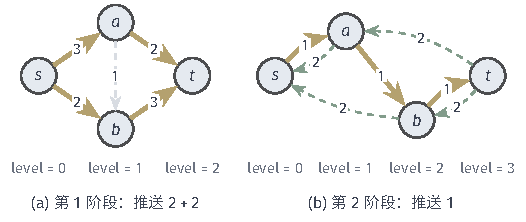
\includegraphics[width=89.129mm]{figures/01-basic-mathematics/04-graphs/tikz/c3-dinic-phases/figure.pdf}
  \caption{Dinic算法在$3,2,1,2,3$网络上的两个阶段，顶点按层数从左到右排列，弧旁为残量。(a) 第$1$阶段：同层边$a\to b$（灰色虚线）不可用，沿两条两弧路径（黄色）各推送$2$。(b) 第$2$阶段：绿色虚线为反向残量，沿$s\to a\to b\to t$推送$1$。}
  \label{fig:graph-opt-dinic-phases}
\end{figure}

\subsection{算法流程}

\paragraph{算法状态与初始化}
例中给每个点标了层数，又依次尝试它的出边。算法要记住的正是这两件事：每个点本轮处于第几层，邻接表试到了哪里。层数约束推进方向，进度让失败的方向不再重试；重新分层后可用边变了，进度只在阶段内保留。算法维护：
\begin{itemize}
  \item 残量$r_e$与流值$F$：初值同Edmonds--Karp算法，跨阶段保留；
  \item 层数$\mathrm{level}(v)$：每个阶段开始时由广度优先遍历重算，不可达的顶点没有层数；
  \item \term{当前弧}（current arc）指针$\mathrm{ptr}(u)$：指向$u$的邻接表中下一条待试的残量边，每个阶段开始时复位到表头，阶段内只向后移。
\end{itemize}

\paragraph{分层与阻塞流计算}
外层循环每个阶段先做广度优先遍历求$\mathrm{level}$，$t$不可达就结束。随后反复从$s$做一次深度优先推送$\mathrm{Push}(s,+\infty)$。

$\mathrm{Push}(u,f)$表示“从$u$出发、手里最多带着$f$，试着送一条路到$t$”，返回实际送达的量：$u=t$时返回$f$；否则从$\mathrm{ptr}(u)$起依次检查边$e=(u\to v)$，满足$r_e>0$与$\mathrm{level}(v)=\mathrm{level}(u)+1$时递归调用$\mathrm{Push}(v,\min\{f,r_e\})$。递归送达$d>0$时，回程中成对更新$r_e$与$r_{\bar e}$并把$d$逐层返回。$\mathrm{Push}(s,+\infty)$返回$0$时，本阶段结束。

指针何时前移，决定搜索既不漏、也不重复：
\begin{itemize}
  \item 跳过：$r_e=0$，或$\mathrm{level}(v)\neq\mathrm{level}(u)+1$，或递归$\mathrm{Push}(v,\cdot)$返回$0$，说明本阶段从这条边已到不了$t$，令$\mathrm{ptr}(u)$前移；
  \item 保留：递归成功时不前移，因为这条边可能还有残量，下一次推送还能用；若它这次被用尽，下次来到$u$时会因$r_e=0$而跳过。
\end{itemize}
指针若在每次推送时清零，失败的分支会被反复搜索；若成功后无条件前移，又会丢掉仍有残量的边。

\begin{algorithm}[Dinic算法]
\label{alg:graph-opt-dinic}
输入：用残量边对存储的流网络，源点$s$，汇点$t$。输出：流值$F$、各原弧流量与割$(S,\bar S)$。
\begin{enumerate}
  \item 正向边$r_e=c_{u,v}$，反向边$r_{\bar e}=0$；$F=0$。
  \item 从$s$只经$r_e>0$的边做广度优先遍历，求$\mathrm{level}$。若$t$不可达，令$S$为可达顶点集，原弧流量取其反向边的残量，输出并停止。
  \item 对每个顶点$u$令$\mathrm{ptr}(u)$指向其邻接表表头。
  \item 令$d=\mathrm{Push}(s,+\infty)$。若$d>0$，置$F\gets F+d$，重复本步；否则回到第2步。
\end{enumerate}
$\mathrm{Push}(u,f)$：
\begin{enumerate}
  \item 若$u=t$，返回$f$。
  \item 当$\mathrm{ptr}(u)$尚未越过表尾时，取其所指的边$e$，终点为$v$：若$r_e>0$且$\mathrm{level}(v)=\mathrm{level}(u)+1$，令$d=\mathrm{Push}(v,\min\{f,r_e\})$；若$d>0$，置$r_e\gets r_e-d$、$r_{\bar e}\gets r_{\bar e}+d$，返回$d$。其余情形令$\mathrm{ptr}(u)$前移一位。
  \item 返回$0$。
\end{enumerate}
\end{algorithm}

递归深度不超过$n-1$；必要时可用显式栈按同样规则前进与回退。

\paragraph{运行示例}
继续$3,2,1,2,3$的网络，边对按同样次序登记，于是$a$的邻接表依次是$a\to s$（反向）、$a\to b$、$a\to t$，$b$的依次是$b\to s$、$b\to a$（均为反向）、$b\to t$。
\begin{itemize}
  \item 第$1$阶段分层：$\mathrm{level}(s,a,b,t)=(0,1,1,2)$，全部指针在表头。
  \item 第$1$次推送：$s$试$s\to a$可用，进入$a$。$a\to s$残量为$0$，跳过；$a\to b$通向同层，跳过；$a\to t$可用，到达$t$。送$\min\{3,2\}=2$，$\mathrm{ptr}(a)$停在$a\to t$，$F=2$。
  \item 第$2$次推送：$s\to a$仍有残量$1$，进入$a$；$a\to t$已耗尽，$\mathrm{ptr}(a)$越过表尾，返回$0$。$s$因此跳过$s\to a$，本阶段不再尝试；改试$s\to b$，$b$跳过两条反向边，经$b\to t$送$\min\{2,3\}=2$，$F=4$。
  \item 第$3$次推送：$s\to b$已耗尽，$\mathrm{ptr}(s)$越过表尾，返回$0$，阻塞流为$4$。
  \item 第$2$阶段分层：残量网络中$s\to a$剩$1$，$a\to b$剩$1$，$b\to t$剩$1$，层数变为$(0,1,2,3)$；指针全部复位。上一阶段放弃的$s\to a$又被尝试。
  \item 第$1$次推送：$s\to a$，$a$跳过$a\to s$后经$a\to b$进入$b$，$b$跳过两条反向边后经$b\to t$到达$t$，送$1$，$F=5$。第$2$次推送返回$0$，阶段结束。
  \item 第$3$次分层：$s$的出边都已耗尽，$t$不可达，停止，$S=\{s\}$，割容量$3+2=5$等于流值。
\end{itemize}
同一输入上，Edmonds--Karp算法要做三次成功的遍历（$s\to a\to t$、$s\to b\to t$、$s\to a\to b\to t$），Dinic算法只用两个成功的阶段；两者都另有一次失败的遍历，给出同一个最小割。

\subsection{正确性与复杂度}

例中第$1$阶段后只能走三弧的路。一般地，完成一个阻塞流后汇点的残量距离严格增加；这以“阶段内的推送确实形成阻塞流”为前提。

每次成功的$\mathrm{Push}(s,+\infty)$沿$L_{\bm x}$中的一条$s$--$t$路径送出该路径的残量最小值（递归中逐层取$\min$），按引理~\ref{lem:graph-opt-augment}，流保持可行，流值增加送出的量。

阶段内，送流使路径上可用边的残量减少，同时让反向边获得残量；但反向边从第$i+1$层指向第$i$层，不是可用边。所以阶段内可用边只会减少，不会新增。由此，从$v$一旦到不了$t$，整个阶段都到不了，被跳过的边不会重新有用。图~\ref{fig:graph-opt-dinic-phases}(b)中的绿色反向残量都是第$1$阶段产生的，按该阶段的层数全指向低一层，不会为失败的分支开出新路。

当$\mathrm{Push}(s,+\infty)$返回$0$时，$s$的每条边都已被跳过，从$s$沿剩余可用边到不了$t$，即阶段开始时$L_{\bm x}$中每条$s$--$t$路径都含一条已被用尽的边，本阶段送出的总流是阻塞流。

\begin{lemma}[阶段距离严格增加]
\label{lem:graph-opt-dinic-distance}
设$\bm x'$由$\bm x$加上$L_{\bm x}$的一个阻塞流得到。若$t$在$\mathcal G_{\bm x'}$中可达，则$h_{\bm x'}(t)>h_{\bm x}(t)$。
\end{lemma}

\begin{proof}
记$\ell=h_{\bm x}$为阶段开始时的层数。$\mathcal G_{\bm x'}$中的残量弧$u\to v$只有两种来源：阶段开始时已在$\mathcal G_{\bm x}$中，由层数定义有$\ell(v)\leq\ell(u)+1$；或者是阶段内送流产生的反向弧，其反向是可用边，有$\ell(v)=\ell(u)-1$。总之每条残量弧$u\to v$都满足
\[
  \ell(v)\leq\ell(u)+1.
\]
于是$\mathcal G_{\bm x'}$中任一条$s$--$t$路径每走一步层数至多加一，弧数至少为$\ell(t)-\ell(s)=h_{\bm x}(t)$。

若恰好相等，路径上每一步都必须使层数加一，因而每条弧都是阶段开始时的可用边，并且送流后仍有残量；这条路就是$L_{\bm x}$中一条未被堵住的$s$--$t$路径，与阻塞流的定义矛盾。所以$h_{\bm x'}(t)>h_{\bm x}(t)$。
\end{proof}

\begin{theorem}[Dinic算法的正确性与开销]
\label{thm:graph-opt-dinic}
在有限实容量的流网络上，Dinic算法至多经过$n-1$个阶段就停止，输出最大流与最小割。使用当前弧指针时，每个阶段用时$O(na)$，总时间为$O(n^2a)$，存储为$O(n+a)$。
\end{theorem}

\begin{proof}
汇点可达时距离在$1$到$n-1$之间，由引理~\ref{lem:graph-opt-dinic-distance}每个阶段至少加一，所以至多$n-1$个阶段后$t$不可达，算法停止。停止时没有增广路径，由定理~\ref{thm:graph-opt-augmenting-path}输出最大流与最小割。

一个阶段内，广度优先遍历用时$O(n+a)$。每次成功推送至少用尽一条可用边，而可用边在阶段内只减不增，所以成功推送至多$2a$次。

考察一次$\mathrm{Push}(s,+\infty)$检查的边：每条被检查的边要么使某个指针前移，要么位于本次成功送达的路径上。指针在一个阶段内总共前移至多$2a$次；成功路径至多$n-1$条弧，共至多$2a$条路径。加上每次调用的常数开销，一个阶段的用时为
\[
  O\bigl(2a+2a(n-1)+n+a\bigr)=O(na).
\]
乘以至多$n-1$个阶段，总时间$O(n^2a)$；另计线性预处理。除残量边对外只多存$\mathrm{level}$与$\mathrm{ptr}$，存储为$O(n+a)$。
\end{proof}

这也给出最大流最小割定理的另一种构造性证明。在单位容量的二部网络上，阶段数还能进一步压低，第~\ref{sec:graph-opt-hopcroft-karp}小节说明这一更强的界。

\section{方法比较与结果检验}
\label{sec:graph-opt-max-flow-analysis}

两种算法共用残量边对与增广更新，差别在于一次遍历之后做多少工作：Edmonds--Karp算法只确定一条最短路，状态只需前驱边；Dinic算法建立整个分层网络，用当前弧指针连续推送到所有最短路被堵住，多存层数与指针。理论界分别为$O(na^2)$与$O(n^2a)$，弧多于顶点时后者较小；但这是最坏情形的上界，不能直接当成实测排名。

算法应输出流$\bm x$、残量可达集确定的割$(S,\bar S)$及共同的数值。检验时逐项核对：每条弧满足$0\leq x_{u,v}\leq c_{u,v}$；每个中间顶点流入等于流出；源点净流出与汇点净流入相等；割容量按跨出弧重新求和，并与流值比较。两者相等时，由引理~\ref{lem:graph-opt-weak-duality}，流与割同时最优，检验不依赖算法过程。

最小割不一定唯一：在$3,2,1,2,3$的网络中，$S=\{s\}$、$\{s,a\}$、$\{s,a,b\}$的割容量都是$5$，只有$S=\{s,b\}$为$6$；残量可达集给出的是源侧最小的一个。

采用浮点数时，应分别报告守恒误差、容量违反量以及流值与割容量之差，不能把近似满足称为精确证书。

后面的问题都要先转成某种网络再使用这里的结论。第~\ref{sec:graph-matching}节的二部图匹配对应单位容量网络，可直接维护匹配；第~\ref{sec:graph-min-cost-flow}章再把各点的供需与每条弧的费用纳入一般模型；第~\ref{chap:pairwise-binary-minimization}章把一类二值变量的成对目标写成割容量，再用最小割求解。这些转换关系必须逐一建立，不能因都画在图上就共享最优性结论。

\FloatBarrier
\section{本章小结}
\label{sec:max-flow-summary}

章首提出两个问题：怎样逐步改进一个输送方案，怎样确认它已不能再改进。第二个问题由割回答。流值等于跨过任意$s$--$t$割的净流量，所以不超过割容量；一个流与一个割数值相等时，两者同时最优，检查者只需逐弧核对容量、守恒与割容量。

第一个问题由残量网络回答。每条原弧对应一条可追加的正向残量弧和一条可撤回的反向残量弧，改进统一为沿增广路径推送瓶颈容量。没有增广路径时，残量网络中从$s$可达的顶点集给出一个与流值相等的割，这就是增广路径判据。由此得到最大流最小割定理：在有限非负实容量的网络中，最大流存在，最大流值等于最小割容量。

能否有限步停下来，取决于选路规则。整数容量下任意选路都会停止，并给出整数最大流；一般实容量下任意选路可能永不停止。Edmonds--Karp算法每次选弧数最少的增广路径，残量层数不减，于是同一条弧不能频繁成为瓶颈，增广至多$na$次，总时间$O(na^2)$。Dinic算法在分层网络中求阻塞流，每个阶段使汇点距离严格增加，配合当前弧指针得到$O(n^2a)$。这些都是最坏情形的上界，不能直接当成实测排名。

本章的网络与证书会在后面反复使用。下一章的二部图匹配是单位容量的最大流，Hopcroft--Karp算法把Dinic算法的分层思想用到配对上；第~\ref{chap:min-cost-flow}章再给残量弧配上费用；第~\ref{chap:pairwise-binary-minimization}章则把一类二值变量的成对目标写成割容量，用最小割求出精确的最优配置。

% 第6章：二部图匹配与指派（章引言；二部图匹配；指派与带权二部图匹配；本章小结）。

\chapter{二部图匹配与指派}
\label{chap:bipartite-matching-assignment}

把若干任务分给若干名人员，只有具备资格的人才能接相应的任务，每人至多接一项、每项至多一人负责。这类问题有两种提法：一种只问最多能配上多少对；另一种要求每个人都分到任务，而不同配对的花费不同，要在全部完整配对中选总成本最低的一个。本章依次回答这两个问题，并给出不必相信求解过程、就能核对结果最优的证据。

第~\ref{sec:graph-matching}节处理配对数量。每人、每项任务至多用一次，与每条弧至多通过一单位流量是同一种限制，所以最大匹配就是第~\ref{chap:max-flow-min-cut}章单位容量网络上的最大流。残量网络中的增广路径落到二部图上，成为新旧配对交替的路径；匈牙利算法只记录配对伙伴，逐个为人员寻找这样的路径。由于逐条贪心加边可能停在“不能再加、却不是最多”的结果上，这一节要特别区分极大匹配与最大匹配。

第~\ref{sec:graph-assignment}节加入成本，研究指派问题。给每行和每列各配一个数，可以得到全部完整指派成本的共同下界；只用恰好达到下界的边完成的指派就是最优的。KM算法在这些边上扩大匹配、受阻时抬高下界，结束时给出精确的证书；Auction算法让行为列出价，用价格协调争抢，结果的误差由一个参数控制。两种算法的保证不同，比较时须先固定条件。

本章的二部图记为$\mathcal G=(L\cup R,E)$。第~\ref{sec:graph-matching}节记$n=|L|+|R|$、$m=|E|$，第~\ref{sec:graph-assignment}节记指派两侧的规模为$r$。

% 第6章第1节：二部图匹配（问题；与单位容量最大流的对应；匈牙利算法与分层改进；结果检验）。

\section{二部图匹配}
\label{sec:graph-matching}

本节只数配对，不考虑成本：在允许的“人员—任务”配对中选出一组，任何人员或任务都不出现在两个配对里，使配对数量最多。第~\ref{sec:graph-opt-match-problem}小节给出二部图与匹配的定义，并用一个小例子说明“不能再加边”不等于“配对最多”。第~\ref{sec:graph-opt-match-alternating}小节把匹配写成单位容量网络上的整数流，由此得到交替路径形式的最优判据。

第~\ref{sec:graph-opt-match-algorithm}小节的匈牙利算法直接利用这一判据，只维护伙伴数组，逐个为左侧顶点寻找增广路径；第~\ref{sec:graph-opt-match-analysis}小节说明怎样核对一个声称的最大匹配。

\subsection{二部图匹配问题}
\label{sec:graph-opt-match-problem}

人员与任务分属两类，资格关系只跨类连接。若无向图的顶点集能分成不相交的两部分$L$与$R$，使每条边恰有一个端点在$L$、另一个端点在$R$，就称它为\term{二部图}（bipartite graph），记作$\mathcal G=(L\cup R,E)$，并称$L$为左侧、$R$为右侧。边$\{u,w\}$（$u\in L$，$w\in R$）简记为$(u,w)$，称为允许边。一组配对合法，是指选出的边两两没有公共端点。

\begin{definition}[匹配]
\label{def:graph-opt-matching}
图$\mathcal G=(V,E)$中两两没有公共端点的边组成的集合$M\subseteq E$称为一个\term{匹配}（matching）。若$(u,w)\in M$，称$u$与$w$被$M$匹配，互为\emph{伙伴}；不被任何匹配边关联的顶点称为自由顶点。边数最多的匹配称为\term{最大匹配}（maximum matching），没有自由顶点的匹配称为\term{完美匹配}（perfect matching）。不能再加入任何一条边而仍为匹配的$M$称为\term{极大匹配}（maximal matching）。
\end{definition}

最大匹配一定是极大匹配，反之不然。设左侧为$a,b$，右侧为任务$1,2$，允许边为$(a,1)$、$(a,2)$、$(b,1)$，如图~\ref{fig:graph-opt-match-maximal-maximum}。若先选$(a,1)$，另两条边都与它共享端点，无法再加，所以$\{(a,1)\}$是极大匹配；可是$\{(a,2),(b,1)\}$有两条边，是最大匹配，也是完美匹配。从前者到后者不能继续加边，只能把$a$改派到任务$2$，腾出任务$1$给$b$。逐条贪心加边可能停在这样的结果上，改进必须允许重排已有的配对。

\begin{figure}[!htb]
  \centering
  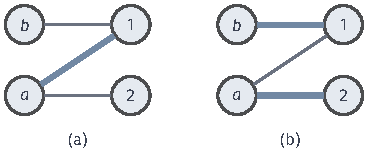
\includegraphics[width=67.515mm]{figures/01-basic-mathematics/04-graphs/tikz/c3-match-maximal-maximum/figure.pdf}
  \caption{极大匹配与最大匹配。细线为允许边，粗蓝线为匹配边。(a)极大匹配$\{(a,1)\}$；(b)最大匹配$\{(a,2),(b,1)\}$，由(a)到(b)须改动已有配对。}
  \label{fig:graph-opt-match-maximal-maximum}
\end{figure}

本节只最大化配对数$|M|$，边上没有成本；成本问题留到第~\ref{sec:graph-assignment}节。两侧大小可以不同，最大匹配至多有$\min\{|L|,|R|\}$条边，但未必达到：若两名人员都只会同一项任务，至多一人能配上。后面的构造利用给定的两侧划分；含奇数长环（如三角形）的一般图无法这样划分，不能直接套用。记$n=|L|+|R|$，$m=|E|$。

\subsection{匹配与最大流的对应}
\label{sec:graph-opt-match-alternating}

由二部图构造流网络：增加源点$s$与汇点$t$，从$s$向每个$u\in L$连弧，把每条允许边$(u,w)$改为弧$u\to w$，再从每个$w\in R$向$t$连弧，所有容量都为$1$，如图~\ref{fig:graph-opt-match-flow-network}。

给定匹配$M$，沿每条匹配边对应的路线$s\to u\to w\to t$各送一单位，得到流值为$|M|$的整数流。反过来，整数流$\bm x$在每条弧上只取$0$或$1$。左侧顶点$u$只有一条容量为$1$的入弧，由流守恒，它至多有一条流量为$1$的出弧；同理，右侧顶点至多有一条流量为$1$的入弧。所以流量为$1$的中间弧两两不共享端点，构成一个匹配，边数等于流值。

由定理~\ref{thm:graph-opt-integer-termination}，整数容量的网络有整数最大流，因此最大匹配的边数等于这个网络的最大流值。这里只从整数流恢复匹配，分数流量不对应任何一组配对。

\begin{figure}[!htb]
  \centering
  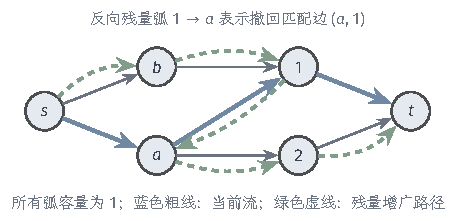
\includegraphics[width=77.093mm]{figures/01-basic-mathematics/04-graphs/tikz/c3-match-flow-network/figure.pdf}
  \caption{图~\ref{fig:graph-opt-match-maximal-maximum}的二部图对应的单位容量网络。蓝色粗弧是匹配$\{(a,1)\}$对应的流；绿色虚线是一条残量$s$--$t$路径，反向残量弧$1\to a$表示撤回$(a,1)$，去掉$s,t$即交替路径$b,1,a,2$。}
  \label{fig:graph-opt-match-flow-network}
\end{figure}

设$\bm x$对应匹配$M$。残量网络中，弧$s\to u$存在当且仅当$u$自由；左侧顶点只能沿未匹配边走到右侧；右侧顶点$w$若自由就走$w\to t$结束，否则只能沿反向残量弧回到伙伴，相当于准备撤回这条匹配边。去掉两端的$s$与$t$，剩下的路径从左到右走未匹配边、从右到左走匹配边。图~\ref{fig:graph-opt-match-flow-network}中的残量路径就是$b,1,a,2$：$b$要任务$1$，请$a$改做任务$2$。

一般地，给定匹配$M$，边交替地不属于$M$与属于$M$的路径称为\term{交替路径}（alternating path）；两个端点都自由的交替路径称为关于$M$的增广路径。在二部图中，增广路径的一端是自由左侧顶点，另一端是自由右侧顶点；首尾两条边都不在$M$中，未匹配边比匹配边多一条。

\begin{lemma}[沿增广路径翻转]
\label{lem:graph-opt-match-flip}
设$P$是关于匹配$M$的增广路径。把$P$上属于$M$的边移出、不属于$M$的边加入，得到的边集$M'$仍是匹配，且$|M'|=|M|+1$。
\end{lemma}

\begin{proof}
$P$外的顶点不受影响。$P$的内部顶点恰关联$P$上一条匹配边和一条未匹配边，且唯一的匹配边就在$P$上，翻转后两者互换，仍恰有一个伙伴。$P$的两个端点原来自由，翻转后各得到一个伙伴。所以$M'$中没有两条边共享端点。$P$上未匹配边比匹配边多一条，故$|M'|=|M|+1$。
\end{proof}

沿残量路径增广一单位，正是沿对应的增广路径翻转，所以最大流的最优性判据可以搬到匹配上。

\begin{theorem}[增广路径判据]
\label{thm:graph-opt-match-augmenting}
二部图中的匹配$M$是最大匹配，当且仅当不存在关于$M$的增广路径。
\end{theorem}

\begin{proof}
若存在增广路径，由引理~\ref{lem:graph-opt-match-flip}可得更大的匹配。反过来，设不存在增广路径，令$\bm x$是$M$对应的流。由上面的对应，残量网络中没有$s$--$t$路径，由定理~\ref{thm:graph-opt-augmenting-path}，$\bm x$是最大流。任何匹配$M''$都对应一个流值为$|M''|$的流，所以$|M''|\leq|M|$。
\end{proof}

这个判据比“不能再加边”强。图~\ref{fig:graph-opt-match-maximal-maximum}(a)中，$\{(a,1)\}$已不能直接加边，却有增广路径$b,1,a,2$；翻转后得到最大匹配$\{(a,2),(b,1)\}$。整体重排能多配一对，是因为中间的顶点只换伙伴，两端的自由顶点各得到一个伙伴。

\subsection{匈牙利算法}
\label{sec:graph-opt-match-algorithm}

定理~\ref{thm:graph-opt-match-augmenting}提示了一种算法：找到增广路径就翻转，找不到就停止。中文教学常把逐个左侧顶点用深度优先搜索找增广路径的做法称为\term{匈牙利算法}（Hungarian algorithm），也称Kuhn算法；英文文献中的Hungarian algorithm通常指第~\ref{sec:graph-assignment}节处理成本的指派算法。它沿用残量增广的思想，但只维护配对关系。

\subsubsection{主要思想}

把图~\ref{fig:graph-opt-match-maximal-maximum}中的$a,b$看成员工甲、乙：甲能做任务$1$和$2$，乙只会任务$1$。甲先接下任务$1$；轮到乙时任务$1$已有人负责，直接找空任务失败。换个问法：先问甲能否改做别的。任务$2$空着，甲改做$2$，空出的任务$1$交给乙。想要的任务已有负责人时，不放弃也不抢走，先替原负责人找去处。

这次调整可以写成$\text{乙}\to1\to\text{甲}\to2$：候选分配、已有分配、候选分配依次交替，终点任务$2$空闲。找到空任务后再逆序落实：甲改做$2$，乙接手$1$。

再增加一名员工和一项任务：甲会$1,2$，乙会$2,3$，丙只会$1$，当前已有甲—1、乙—2。丙想要任务$1$，就请甲另找；甲想要任务$2$，又请乙另找；乙找到空任务$3$。沿$\text{丙}\to1\to\text{甲}\to2\to\text{乙}\to3$连续让位，三人都有了任务，如图~\ref{fig:graph-opt-match-augment}。替甲、替乙找去处是同一个问题，所以可以递归：为某人找任务时，逐个询问他会的任务，任务空着就成功，否则递归地为该任务的负责人另找任务。

\begin{figure}[!htb]
  \centering
  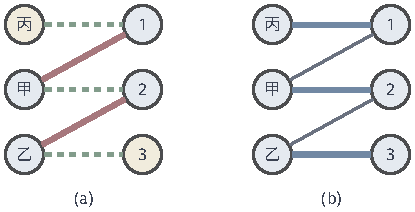
\includegraphics[width=101.279mm]{figures/01-basic-mathematics/04-graphs/tikz/c3-match-augment/figure.pdf}
  \caption{三人三任务的让位链。(a)当前匹配为甲—1、乙—2，丙与任务$3$自由（黄色），让位链交替经过将加入的边（绿色虚线）与将撤去的匹配边（红线）；(b)翻转后配对数由$2$增为$3$。}
  \label{fig:graph-opt-match-augment}
\end{figure}

把员工和任务还原为左右顶点，成功的让位链就是从自由左侧顶点到自由右侧顶点的增广路径，逆序落实就是引理~\ref{lem:graph-opt-match-flip}的翻转；某个分支失败，原负责人找不到去处，原匹配应保持不变。与最大流归约相比，这里只用伙伴数组，省去源汇、容量和残量弧，但这只减少状态，不保证渐近界更优\scite{math-graph-sedgewick-bipartite-matching}。

\subsubsection{算法流程}

\paragraph{算法状态与初始化}
手工调整要记两件事：谁现在负责哪项任务；本轮哪些任务已经问过。前者成功改配后改变并跨轮保留；后者只属于本轮，重问只会重复同样的结果。邻接表在运行前给定、运行中不变，不算状态。取较小的一侧作为左侧，记其顶点数为$p$，算法维护：
\begin{itemize}
  \item 伙伴数组$\mu_L(u)$与$\mu_R(w)$：左右顶点的当前伙伴，初值全为空，即$M=\varnothing$；
  \item 访问时间戳$\tau(w)$：右侧顶点$w$最近一次被询问时的轮次，初值全为$0$；
  \item 当前轮次$k$：初值为$0$。
\end{itemize}
每处理一个左侧顶点就令$k\gets k+1$，本轮已问过的恰是$\tau(w)=k$的右侧顶点，旧标记自动失效，不必清空。新处理的左侧顶点从未被询问，总是自由的。

\paragraph{搜索与改配}
为左侧顶点$u$寻找增广路径的过程$\mathrm{Try}(u)$按邻接表扫描$u$的邻居$w$：
\begin{itemize}
  \item 若$\tau(w)=k$：本轮已问过，跳过；
  \item 否则令$\tau(w)\gets k$。若$w$自由，或递归调用$\mathrm{Try}(\mu_R(w))$成功，就令$\mu_R(w)\gets u$、$\mu_L(u)\gets w$，返回成功；否则继续扫描下一个邻居。
\end{itemize}
邻居扫描完仍未成功，返回失败。伙伴只在成功分支上改写，所以整轮失败时原匹配完整保留。外层对每个左侧顶点依次调用$\mathrm{Try}$，处理完即停止。

成功时改写从链尾向链头逐层进行：内层先为靠后的员工记下新任务，外层才把前一项任务改记给新负责人。两步之间，该任务在$\mu_R$中仍记着原负责人，而原负责人在$\mu_L$中已记着新任务；回到链头时两数组重新一致，所以匹配只在一轮结束后对外使用。

\begin{algorithm}[匈牙利算法]
\label{alg:graph-opt-augmenting-matching}
输入：二部图的左侧邻接表，左侧为较小的一侧。输出：最大匹配的伙伴数组。
\begin{enumerate}
  \item 令全部伙伴为空，全部$\tau(w)=0$，$k=0$。
  \item 对左侧顶点$u$依次执行：令$k\gets k+1$，调用$\mathrm{Try}(u)$。
  \item 输出$\mu_L,\mu_R$。
\end{enumerate}
过程$\mathrm{Try}(u)$：对$u$的每个邻居$w$，若$\tau(w)=k$则跳过；否则令$\tau(w)\gets k$，若$\mu_R(w)$为空或$\mathrm{Try}(\mu_R(w))$返回成功，令$\mu_R(w)\gets u$、$\mu_L(u)\gets w$并返回成功。全部邻居扫描完后返回失败。
\end{algorithm}

\paragraph{运行示例}
表~\ref{tab:graph-opt-match-trace}按“询问—递归—成功返回—改配”逐行列出两个例子，邻居按编号读取。三任务例多递归一层，做法不变；其下半第$3$行$\mu_R$把任务$2,3$都记在乙名下，正是上述暂时不对应。

\begin{table*}[!htb]
  \centering\small
  \caption{匈牙利算法的运行。上半为两任务例，下半为三任务例的第$3$轮（前两轮已得甲—1、乙—2）。$\tau$与$\mu_R$按任务编号列出，“—”表示空。}
  \label{tab:graph-opt-match-trace}
  \begin{tabular}{@{}cllll@{}}
    \toprule
    轮 & 调用栈 & 动作 & $\tau$ & $\mu_R$ \\
    \midrule
    $1$ & 甲 & 问$1$：空闲，记甲—1，成功 & $(1,0)$ & (甲,—) \\
    $2$ & 乙 & 问$1$：甲负责，为甲递归 & $(2,0)$ & (甲,—) \\
    $2$ & 乙，甲 & 跳过$1$；问$2$：空闲，记甲—2，成功 & $(2,2)$ & (甲,甲) \\
    $2$ & 乙 & 收到成功，记乙—1 & $(2,2)$ & (乙,甲) \\
    \midrule
    $3$ & 丙 & 问$1$：甲负责，为甲递归 & $(3,2,0)$ & (甲,乙,—) \\
    $3$ & 丙，甲 & 跳过$1$；问$2$：乙负责，为乙递归 & $(3,3,0)$ & (甲,乙,—) \\
    $3$ & 丙，甲，乙 & 跳过$2$；问$3$：空闲，记乙—3，成功 & $(3,3,3)$ & (甲,乙,乙) \\
    $3$ & 丙，甲 & 收到成功，记甲—2 & $(3,3,3)$ & (甲,甲,乙) \\
    $3$ & 丙 & 收到成功，记丙—1 & $(3,3,3)$ & (丙,甲,乙) \\
    \bottomrule
  \end{tabular}
\end{table*}

失败的搜索要保留原匹配。在三任务例中删去允许边甲—2，前两轮仍得到甲—1、乙—2，第$3$轮为：
\begin{itemize}
  \item 丙询问任务$1$，令$\tau(1)=3$，任务$1$由甲负责，为甲递归；
  \item 甲只会任务$1$，而它本轮已问过，甲的搜索失败，不改任何记录；
  \item 丙再无别的任务可问，整轮失败。
\end{itemize}
伙伴数组仍是甲—1、乙—2。若丙询问时就先撤去甲—1，甲、丙都将没有任务，匹配反而少一对。

\subsubsection{正确性与复杂度}

在三人让位链上数配对：甲、乙只换了任务，丙和任务$3$各得到伙伴，恰好多$1$对，一般情形即引理~\ref{lem:graph-opt-match-flip}。还需说明搜索失败时当前匹配已不能改进。

\begin{theorem}[匈牙利算法的正确性]
设左侧顶点按$u_1,\ldots,u_p$的顺序处理，$\mathcal G_k$为由$u_1,\ldots,u_k$与全部右侧顶点导出的子图。处理完$u_k$后，伙伴数组给出$\mathcal G_k$的一个最大匹配；特别地，算法输出$\mathcal G$的最大匹配。
\end{theorem}

\begin{proof}
对$k$归纳，$k=0$时匹配为空，结论成立。设处理$u_k$前的匹配$M$是$\mathcal G_{k-1}$的最大匹配，$u_k$是自由顶点。$\mathcal G_k$只比$\mathcal G_{k-1}$多一个顶点$u_k$，任何匹配中至多一条边含$u_k$，所以$\mathcal G_k$的最大匹配数至多比$\mathcal G_{k-1}$的多$1$。

若$\mathrm{Try}(u_k)$成功，递归链依次经过$u_k$、右侧顶点$w_1$、$w_1$的伙伴、右侧顶点$w_2$、……，止于一个自由右侧顶点。本轮每个右侧顶点至多问一次，链上的左侧顶点互不相同，所以这条链是增广路径，逐层改写就是翻转。由引理~\ref{lem:graph-opt-match-flip}，新匹配有$|M|+1$条边，达到上述上界，是$\mathcal G_k$的最大匹配。

若$\mathrm{Try}(u_k)$失败，伙伴数组未变。记本轮被询问过的右侧顶点集为$R^*$，$L^*$由$u_k$与$R^*$中顶点的伙伴组成。被询问的右侧顶点都不自由，本轮对其伙伴调用过$\mathrm{Try}$，失败的$\mathrm{Try}$扫描了全部邻居，所以$L^*$中每个顶点的邻居都在$R^*$中。于是从$u_k$出发的交替路径始终留在$L^*\cup R^*$中，到不了自由右侧顶点。假如$M$不是$\mathcal G_k$的最大匹配，由定理~\ref{thm:graph-opt-match-augmenting}存在增广路径$P$。$P$的内部顶点都已匹配，不会是自由的$u_k$；若$u_k$也不是$P$的端点，$P$就整条位于$\mathcal G_{k-1}$中，与$M$在$\mathcal G_{k-1}$中最大矛盾。所以$P$从$u_k$出发，而这刚被排除。故$M$仍是$\mathcal G_k$的最大匹配。
\end{proof}

同一轮中每个右侧顶点至多被询问一次，每个左侧顶点至多调用一次$\mathrm{Try}$（它是$u_k$，或某个被询问右侧顶点的伙伴），所以每条允许边至多扫描一次，一轮为$O(1+m)$。$p$轮共$O(p+pm)$，加上伙伴数组与时间戳的初始化$O(n)$，总时间为$O(n+pm)$；邻接表、伙伴数组与时间戳共占$O(n+m)$空间。若每轮清空访问数组，另需$O(|R|)$；用邻接矩阵时每次扫描要读整行，也须另算代价。

\subsubsection{分层增广的进一步改进}
\label{sec:graph-opt-hopcroft-karp}

逐点搜索每轮至多找到一条增广路径。Hopcroft--Karp算法把第~\ref{sec:graph-opt-dinic}节Dinic算法的分层思想用到单位容量网络上，每个阶段做两步：
\begin{itemize}
  \item 分层：从全部自由左侧顶点同时沿交替路径做广度优先遍历，求出最短增广路径长度与各顶点层号；
  \item 增广：只沿层号逐层加一的边做深度优先搜索，找出一组极大的、顶点互不相交的最短增广路径，一起翻转。
\end{itemize}
这组路径就是分层残量网络中的阻塞流（定义~\ref{def:graph-opt-blocking-flow}），与Dinic算法同理，每个阶段之后最短增广路径的长度严格增加。

阶段数很少，理由简述如下：$\sqrt n$个阶段之后，最短增广路径已有超过$2\sqrt n$条边；当前匹配与任一最大匹配的差可以分解为顶点互不相交的增广路径，每条都占去超过$\sqrt n$个顶点，所以至多还差$\sqrt n$条，至多再需$\sqrt n$个阶段。合计$O(\sqrt n)$个阶段，每阶段为$O(m)$，主计算为$O(m\sqrt n)$；孤立顶点不在任何增广路径上，先用$O(n)$时间删去，总时间写作$O(n+m\sqrt n)$\scite{math-graph-sedgewick-hopcroft-karp}。这个界不适用于前面逐点搜索的实现。

\subsection{结果检验}
\label{sec:graph-opt-match-analysis}

先确认可行性：所选边都是允许边，两两没有公共端点，再重数边数；伙伴数组还应两两对应，即$\mu_L(u)=w$当且仅当$\mu_R(w)=u$。

最大性另需证据：可以从全部自由左侧顶点重做一次交替搜索，确认到不了自由右侧顶点；更独立的证据是单位容量网络中容量等于$|M|$的割。

令$Z$为从自由左侧顶点沿交替路径能到达的顶点集，若其中没有自由右侧顶点，取源侧$S=\{s\}\cup Z$。这时$Z$中左侧顶点的邻居都在$Z$中，$Z$中的右侧顶点都已匹配且伙伴也在$Z$中，所以跨出$S$的弧只有$s\to u$（$u\in L\setminus Z$）与$w\to t$（$w\in R\cap Z$）。对每条匹配边$(u,w)$，$u\in Z$时恰有$w\to t$跨出，$u\notin Z$时$w\notin Z$，恰有$s\to u$跨出；自由顶点不贡献跨出的弧。故割容量为$|M|$，由引理~\ref{lem:graph-opt-weak-duality}，任何匹配对应的流值都不超过$|M|$，$M$最大。

在删去甲—2的例子中，$Z=\{\text{丙},1,\text{甲}\}$，跨出$S$的弧是$s\to\text{乙}$与$1\to t$，割容量为$2$，等于匹配的边数。

不能因为自由顶点之间没有允许边就宣布最大：图~\ref{fig:graph-opt-match-maximal-maximum}(a)中自由的$b$与$2$不相邻，却仍有增广路径。

完整配对可能有多种，数量无法区分优劣。第~\ref{sec:graph-assignment}节给配对加上成本，选出总成本最小的完整配对。

% 第6章第2节：指派与带权二部图匹配（指派问题；可行标号与紧边证书；KM算法及矩形、不完整配对；Auction算法及误差缩放；方法比较与结果检验）。

\section{指派与带权二部图匹配}
\label{sec:graph-assignment}

上一节只关心能配上多少对。若每名员工都必须分到一项任务、不同配对花费不同，就要在全部完整配对中挑总成本最低的一个。逐人挑最便宜的任务会让几个人挤向同一项任务，所以需要判断“谁让出偏爱的任务更划算”，并证明得到的方案已经最省。

给每名员工和每项任务各配一个数，可以得到任何完整配对成本的下界；只用恰好达到下界的边完成的配对就是最优的。KM算法保持下界有效，在这些边上用交替路径扩大匹配，受阻时抬高下界；Auction算法让员工为任务出价，用价格协调争抢，得到误差可控的方案。

\subsection{指派问题}
\label{sec:graph-opt-assign-problem}

把员工看成二部图左侧的行，任务看成右侧的列。行$i$与列$j$允许配对时，两者之间有一条边，成本$c_{i,j}$是有限实数，可以为负；不允许的配对没有边。

\begin{definition}[指派问题]
\label{def:graph-opt-assignment}
设二部图两侧各有$r$个顶点，左侧为行$1,\ldots,r$，右侧为列$1,\ldots,r$，允许的行列对组成边集$E$，每条边$(i,j)\in E$有有限实成本$c_{i,j}$。\term{指派问题}（assignment problem）要求选出一个只用允许边的完美匹配，即给每行$i$指定一个不同的列$\sigma(i)$，使总成本
\begin{equation}
  C(\sigma)=\sum_{i=1}^r c_{i,\sigma(i)}
  \label{eq:graph-opt-assignment-cost}
\end{equation}
最小。
\end{definition}

指派问题也称为最小权完美匹配，输出一个最优指派，或“不存在完美匹配”的结论。若要使收益$w_{i,j}$之和最大，取$c_{i,j}=-w_{i,j}$即可。全部行列对都允许时，$\sigma$可以是任意置换，成本写成$r$阶矩阵$\bm C=(c_{i,j})$。

“每个顶点恰配一次”不能随意放宽。允许匹配任意多对、只求收益最大的是另一个问题，即最大权匹配：负收益的边宁可不选，结果可能只配一部分顶点；在最小成本形式下，成本全为正时空匹配反而“最便宜”。行列数不等、禁配、可以不配但要付惩罚等情形，在第~\ref{sec:graph-opt-assign-rectangular}小节归结为本定义；下文先在方阵上讲算法。

\subsection{可行标号与最优性条件}
\label{sec:graph-opt-assign-labels}

判断一个指派是否最优，不能把$r!$个指派逐一比较，需要一个能对全部指派同时成立的下界。给每行$i$配实数$u_i$，每列$j$配实数$v_j$。若对每条允许边都有
\begin{equation}
  u_i+v_j\leq c_{i,j},
  \label{eq:graph-opt-feasible-labels}
\end{equation}
就称$(\bm u,\bm v)$为\term{可行标号}（feasible labeling）：把成本分摊给行与列，两份之和不超过实际成本。

对任意完整指派$\sigma$，把它用到的$r$条边的不等式相加；每行恰出现一次，每列也恰出现一次，于是
\begin{equation}
  \begin{aligned}
    C(\sigma)=\sum_{i=1}^r c_{i,\sigma(i)}
    &\geq\sum_{i=1}^r\bigl(u_i+v_{\sigma(i)}\bigr)\\
    &=\sum_{i=1}^r u_i+\sum_{j=1}^r v_j.
  \end{aligned}
  \label{eq:graph-opt-assignment-lower-bound}
\end{equation}
右边与$\sigma$无关，是全部完整指派成本的共同下界。这个论证只用到“每行每列恰计一次”，不需要一般的线性规划对偶理论。

从线性规划看，可行标号正是指派问题对偶问题的可行解，下面的紧边条件就是互补松弛；这一解释可参考\BookChapterRef{chap:linear-programming}{第~\ref{chap:linear-programming}章}。

称$c_{i,j}-u_i-v_j\geq0$为边$(i,j)$的剩余量。剩余量为零、使式~\eqref{eq:graph-opt-feasible-labels}取等号的允许边称为\term{紧边}（tight edge），全部顶点与全部紧边组成的子图称为\term{相等子图}（equality subgraph）。
\begin{theorem}[紧边指派的最优性]
\label{thm:graph-opt-tight-assignment}
设$(\bm u,\bm v)$是可行标号。若完整指派$\sigma$只使用紧边，即$\sigma$是相等子图中的完美匹配，则$C(\sigma)=\sum_iu_i+\sum_jv_j$，因而$\sigma$是最优指派。
\end{theorem}

\begin{proof}
$\sigma$用到的每条边都取等号，式~\eqref{eq:graph-opt-assignment-lower-bound}中的求和不等式也取等号，所以$\sigma$的成本等于下界。任何完整指派的成本都不低于这个下界，所以$\sigma$最优。
\end{proof}

可行标号本身只提供下界；相等子图里可能没有完美匹配，不能据此宣布最优。求解因此变成两件同时进行的事：保持标号可行，同时在紧边中凑出完美匹配。KM算法严格按此工作；Auction算法允许所选的边留下一点剩余量，误差在第~\ref{sec:graph-opt-auction}小节给出。

\subsection{KM算法}
\label{sec:graph-opt-hungarian}

\term{KM算法}（Kuhn--Munkres algorithm）以Kuhn和Munkres命名，英文文献通常称为Hungarian algorithm，即带权的匈牙利算法；上一节的匈牙利算法只求最大匹配，没有成本。它从可行标号和空匹配出发，只在紧边上寻找增广路径，受阻时调整标号产生新的紧边。

\subsubsection{主要思想}

沿用上一节的两名员工甲、乙和两项任务$1$、$2$，现在每个配对都允许，但成本不同：
\[
  \bm C=\begin{bmatrix}1&2\\1&4\end{bmatrix},
\]
行依次为甲、乙，第$j$列是任务$j$。完整方案只有两个，成本分别为
\[
  \begin{aligned}
    \text{甲—}1,\ \text{乙—}2&:\quad 1+4=5,\\
    \text{甲—}2,\ \text{乙—}1&:\quad 2+1=3.
  \end{aligned}
\]
两人最便宜的选择都是任务$1$，“每行选最小”拼不成指派；要比较的是让步的代价：甲改做任务$2$多花$1$，乙则多花$3$。

把上一小节的标号放回成本表。从每行最小值出发取$\bm u=(1,1)$、$\bm v=(0,0)$，标号可行，各格剩余量$c_{i,j}-u_i-v_j$为
\[
  \begin{bmatrix}0&1\\0&3\end{bmatrix}.
\]
零格就是紧边。两个零格都在第一列，相等子图暂时没有完美匹配。

让甲先占任务$1$，再从自由的乙出发找增广路径。乙沿紧边到任务$1$，任务$1$已归甲，于是转去问甲；甲除任务$1$外没有紧边，搜索受阻，如图~\ref{fig:graph-opt-km}(a)。

要接到空闲的任务$2$，甲还差$1$、乙还差$3$，所以只把标号推进较小的差额$1$：甲、乙的标号各加$1$，使通往树外的剩余量减$1$；任务$1$的标号减$1$，使树内两条紧边保持为零。新标号为
\[
  \bm u=(2,2),\qquad\bm v=(-1,0).
\]
这时甲到任务$2$变紧，得到增广路径乙—任务$1$—甲—任务$2$，如图~\ref{fig:graph-opt-km}(b)。

翻转后甲做任务$2$、乙做任务$1$，成本等于标号之和：
\[
  c_{\text{甲},2}+c_{\text{乙},1}=2+1=3=2+2+(-1)+0.
\]
由定理~\ref{thm:graph-opt-tight-assignment}，这个指派最优。成本表没有被改写，改变的只是下界的表示。

\begin{figure}[!htb]
  \centering
  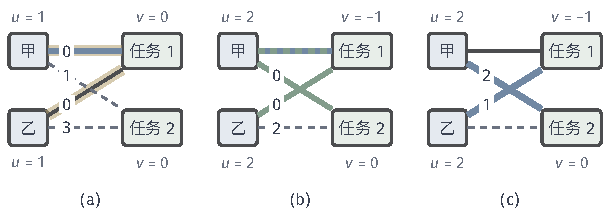
\includegraphics[width=102.799mm]{figures/01-basic-mathematics/04-graphs/tikz/c3-assign-km/figure.pdf}
  \caption{KM算法在成本矩阵$\left[\begin{smallmatrix}1&2\\1&4\end{smallmatrix}\right]$上的运行。顶点旁为标号，(a)(b)边旁为剩余量，(c)边旁为成本；实线为紧边，虚线为非紧边，粗蓝线为匹配。(a)从乙出发的交替树（黄色衬底）受阻，$\delta=1$。(b)调标后甲到任务$2$变紧，出现增广路径（绿色）。(c)指派成本$3$等于标号之和。}
  \label{fig:graph-opt-km}
\end{figure}

这个例子里的做法可以一般化。从一个自由行出发，只沿紧边生长\term{交替树}（alternating tree）：从行走未匹配的紧边到列，到达已匹配的列就沿匹配边回到它的行。记树中的行集为$S$、列集为$T$。

到达自由列就沿树中路径增广；所有紧边都通向$T$时，在$S$到树外列的边中取最小剩余量$\delta$，令$S$中行标号加$\delta$、$T$中列标号减$\delta$。差额更大会违反式~\eqref{eq:graph-opt-feasible-labels}，更小则没有新的紧边。

为了不在每次受阻时重新比较全部边，算法为每个树外列记住“从树中哪一行过来差得最少、差多少”\scite{math-graph-zeh-hungarian}。

\subsubsection{算法流程}

\paragraph{算法状态与初始化}
输入是允许边集与成本，运行中不变，不算状态。对照手算，算法维护以下状态：
\begin{itemize}
  \item 伙伴数组：每行配给的列、每列配给的行，初值全为空。
  \item 标号$\bm u,\bm v$：先检查每行至少有一条允许边，否则直接报告不可行；取$u_i=\min_{j:(i,j)\in E}c_{i,j}$，$v_j=0$。每条允许边满足$u_i+0\leq c_{i,j}$，标号可行，且每行至少有一条紧边。
  \item 交替树：行集$S$、列集$T$，以及每个入树列的前驱行，即把它带进树的那一行。为一个新的自由行建树时，$S$只含该行，$T$为空。
  \item 松弛量与来源：对每个树外列$j$，
  \[
    \mathrm{slack}(j)=\min\bigl\{c_{i,j}-u_i-v_j:\ i\in S,\ (i,j)\in E\bigr\},
  \]
  没有候选时记为$+\infty$；$\mathrm{from}(j)$记录取到最小值的行。建树时按根行的允许边初始化。
\end{itemize}
调标后交替树和来源记录都保留，只有增广成功后，才为下一个自由行重建这些状态。

\paragraph{扩树、调标与增广}
为一个自由行建树后，按情形反复执行：
\begin{itemize}
  \item 扩树：若有树外列$j$满足$\mathrm{slack}(j)=0$，就把$j$加入$T$，前驱记为$\mathrm{from}(j)$。若$j$已匹配，把它的行$i'$加入$S$，再只扫描$i'$的允许边，用$c_{i',j'}-u_{i'}-v_{j'}$更新各树外列的$\mathrm{slack}(j')$与$\mathrm{from}(j')$。
  \item 增广：若加入$T$的$j$是自由列，从$j$沿前驱和匹配边回溯到根，得到一条全由紧边组成的增广路径；翻转路径上的配对，匹配增加一对，本轮结束。
  \item 调标：若树外列的松弛量都为正，取
  \begin{equation}
    \delta=\min_{j\notin T}\mathrm{slack}(j),
    \label{eq:graph-opt-hungarian-delta}
  \end{equation}
  令$S$中各行$u_i\gets u_i+\delta$、$T$中各列$v_j\gets v_j-\delta$，各树外列$\mathrm{slack}(j)\gets\mathrm{slack}(j)-\delta$，来源不变。取到最小值的列松弛量变为零，随即可以扩树。
\end{itemize}
若需要调标时全部树外列的松弛量都为$+\infty$，报告不可行。全部行都匹配时停止，输出匹配与标号。

调标时行在$S$外、列在$T$中的边剩余量增加$\delta$，原来的紧边可能不再紧，相等子图并非只增不减；保留下来的是树中的边和匹配边，下一小节核对。

\begin{algorithm}[KM算法]
\label{alg:graph-opt-hungarian}
输入：两侧各$r$个顶点的允许边集与成本。输出：最优指派与可行标号，或“不可行”。
\begin{enumerate}
  \item 若某行没有允许边，报告不可行；否则置$u_i$为第$i$行最小允许成本、$v_j=0$，伙伴全为空。
  \item 若所有行都已匹配，转第6步。否则取自由行$i_0$，置$S=\{i_0\}$、$T=\varnothing$，对每列$j$置$\mathrm{slack}(j)=c_{i_0,j}-u_{i_0}-v_j$（不允许时为$+\infty$）、$\mathrm{from}(j)=i_0$。
  \item 若有$j\notin T$使$\mathrm{slack}(j)=0$：把$j$加入$T$，前驱置为$\mathrm{from}(j)$。若$j$自由，转第5步；否则把$j$的伙伴行$i'$加入$S$，对每个$j'\notin T$，若$c_{i',j'}-u_{i'}-v_{j'}<\mathrm{slack}(j')$，就更新$\mathrm{slack}(j')$并置$\mathrm{from}(j')=i'$；重复第3步。
  \item 若所有$j\notin T$都有$\mathrm{slack}(j)=+\infty$，报告不可行；否则按式~\eqref{eq:graph-opt-hungarian-delta}求$\delta$，$S$中行标号加$\delta$、$T$中列标号减$\delta$、树外列松弛量减$\delta$，回到第3步。
  \item 从自由列$j$开始，令$i$为$j$的前驱、$j''$为$i$原来的伙伴，把$i$改配给$j$，再令$j\gets j''$，直到$i=i_0$；回到第2步。
  \item 输出伙伴数组与标号$(\bm u,\bm v)$。
\end{enumerate}
\end{algorithm}

\paragraph{运行示例}
表~\ref{tab:graph-opt-hungarian-trace}把上面的手算翻译成状态：
\begin{itemize}
  \item 以甲为根，任务$1$的松弛量为$0$且空闲，直接增广，甲配任务$1$。
  \item 以乙为根，任务$1$入树；它已归甲，甲入树，只扫描甲的边，把任务$2$的松弛量从$3$（来自乙）降为$1$（来自甲）。
  \item 调标$\delta=1$，任务$2$的松弛量变为$0$，来源仍是甲。
  \item 任务$2$入树，前驱为甲；它空闲，回溯：甲改配任务$2$，任务$1$交给其前驱乙。
\end{itemize}
成本$3$等于标号之和，逐行贪心的成本$5$则不然。加入一行只扫描这一行、已有最小值继续保留，正是复杂度分析依赖的增量维护。

\begin{table*}[!htb]
  \centering\small
  \caption{KM算法在成本矩阵$\left[\begin{smallmatrix}1&2\\1&4\end{smallmatrix}\right]$上的状态。每行为动作后的状态；松弛量依次为任务$1$、$2$，括号内为来源，“—”表示已入树。}
  \label{tab:graph-opt-hungarian-trace}
  \begin{tabular}{@{}lllll@{}}
    \toprule
    动作 & $S$；$T$ & $\bm u$；$\bm v$ & 松弛量（来源） & 匹配 \\
    \midrule
    以甲为根建树 & $\{\text{甲}\}$；$\varnothing$ & $(1,1)$；$(0,0)$ & $0$（甲），$1$（甲） & 空 \\
    任务$1$入树，增广 & — & $(1,1)$；$(0,0)$ & — & 甲—$1$ \\
    以乙为根建树 & $\{\text{乙}\}$；$\varnothing$ & $(1,1)$；$(0,0)$ & $0$（乙），$3$（乙） & 甲—$1$ \\
    任务$1$、甲入树 & $\{\text{乙},\text{甲}\}$；$\{1\}$ & $(1,1)$；$(0,0)$ & —，$1$（甲） & 甲—$1$ \\
    调标$\delta=1$ & $\{\text{乙},\text{甲}\}$；$\{1\}$ & $(2,2)$；$(-1,0)$ & —，$0$（甲） & 甲—$1$ \\
    任务$2$入树，增广 & — & $(2,2)$；$(-1,0)$ & — & 甲—$2$，乙—$1$ \\
    \bottomrule
  \end{tabular}
\end{table*}

\subsubsection{正确性与复杂度}

两人例中下界从$2$升到$3$，与方案成本相等。一般情形依赖四件事：初始标号可行；扩树与调标保持标号可行、匹配紧和树中紧；调标后树能继续生长；每次增广增加一对。扩树和增广只沿紧边进行、不改标号，剩下的是调标。

\begin{lemma}[调标的效果]
设标号可行，匹配边与交替树中的边都是紧边，且$\delta$按式~\eqref{eq:graph-opt-hungarian-delta}取有限值。调标后标号仍可行，匹配边与树中的边仍是紧边，至少有一个树外列的松弛量变为零，标号之和增加$\delta$。
\end{lemma}

\begin{proof}
按端点归属逐类检查允许边$(i,j)$的剩余量$c_{i,j}-u_i-v_j$。$i\in S$、$j\in T$时，$u_i$加$\delta$、$v_j$减$\delta$，剩余量不变，树中的紧边都属于这一类。

$i\in S$、$j\notin T$时，剩余量减$\delta$；由$\delta$是这类边剩余量的最小值，减后仍非负，取到最小值的边变为零。$i\notin S$、$j\in T$时剩余量增加$\delta$，其余边不变，所以标号可行。

再看紧边与松弛量。树中每个列都与树中某一行匹配，每个非根行都经匹配边进树，匹配边要么两端都在树中，要么两端都在树外，剩余量都不变，仍为零。树外列的松弛量正是第二类边剩余量的最小值，统一减$\delta$后与新标号一致。

最后，树中每个列都带进一个已匹配的行，根行自由，所以$|S|=|T|+1$，标号之和的增量为
\[
  |S|\delta-|T|\delta=\delta.
\]
\end{proof}

由此，标号可行、匹配只用紧边两条性质在整个运行中保持。算法停止且全部行都匹配时，匹配是相等子图中的完美匹配，由定理~\ref{thm:graph-opt-tight-assignment}，它是最优指派。

报告不可行也是正确的：若树外列的松弛量全为$+\infty$，$S$中各行的允许列全部落在$T$中，$|S|$行只能使用$|T|=|S|-1$个列，不可能各配一个不同的列。

有限终止由计数得到。每次调标后至少有一列入树；若它自由就立即增广，否则它的伙伴行入树。树中的列至多$r$个，所以一个自由行至多经过$r$次调标就增广。每次增广使匹配增加一对，至多$r$次。

对$r$阶稠密成本表，一轮建树中至多$r$行加入$S$，每行扫描并更新松弛量$O(r)$；至多$r$次扩树或调标，每次在树外列中找零或求$\delta$并统一减$\delta$为$O(r)$。一轮为$O(r^2)$，$r$轮共$O(r^3)$次实数运算。

这个界依赖于调标后保留交替树和已有的最小值；若每次受阻都从根重新搜索、重新比较全部边，就不能直接引用它\scite{math-graph-zeh-hungarian-fast}。成本表占$O(r^2)$，是输入本身；伙伴、标号、前驱、松弛量等工作数组为$O(r)$。

\subsubsection{矩形指派与不完整配对}
\label{sec:graph-opt-assign-rectangular}

行数少于列数时，补充到每列成本都为零的虚拟行。虚拟行只占用真实行没用到的列，完整指派的成本等于真实部分的成本，删去虚拟行的配对即得原问题的解。

允许对象不配对、但要付惩罚时，不能只把“恰配一次”放宽成“至多配一次”：成本非负时，什么都不配就成了最优解。正确的做法是把惩罚写进模型。给每个左侧对象$i$配一个专属虚拟列，配给它的成本是$i$不配对的惩罚$\rho_i$；给每个右侧对象$j$配一个专属虚拟行，成本是$j$的惩罚$\eta_j$；真实对象与非专属虚拟对象之间禁止配对，虚拟行与虚拟列之间成本为零。这样补成的方阵中，完整指派的成本恰为真实配对成本加上未配对对象的惩罚。

禁止的配对就是边集$E$中没有的边，在KM算法中不参与行最小值、扩树和松弛量。不要用随手取的“大成本”代替禁止：不够大时算法可能真的选它，够大也把不可行掩盖成高成本的“解”。KM算法在松弛量全为$+\infty$时报告的不可行，对应原模型中某组行能用的列不够。

成本可以为负，行最小值初始化照样成立。所有边成本同加一个常数，完整指派的总成本都变化$r$倍的这个常数，最优解不变；这依赖配对数量固定，在允许不配对的模型中则会改变取舍。算法结束后，先删去或解释虚拟配对，再按原始成本重算真实成本和惩罚。

\subsection{Auction算法}
\label{sec:graph-opt-auction}

\term{Auction算法}（auction algorithm）又称拍卖算法，把行看作竞标者、列看作物品，用物品的价格协调多名竞标者对同一物品的争抢。本节介绍串行前向版本，主线采用$r$阶完整有限成本矩阵，即每个配对都允许。$r=0$时返回空指派，$r=1$时直接返回唯一配对；以下竞价过程假定$r\geq2$。

\subsubsection{主要思想}

仍用同一成本矩阵，甲、乙是竞标者，任务是物品。不加价格时两人都偏好任务$1$；若只是“后来者抢走”，同一物品可以无休止地转手。需要让争抢付出代价：物品越受争抢，继续选它越不划算。为此给每个物品$j$配一个价格$p_j$，竞标者$i$按调整成本$c_{i,j}+p_j$比较物品。

先看甲的第一次出价。零价格下任务$1$、$2$的调整成本是$1$和$2$，相差$1$。若把任务$1$的价格恰好提高$1$，两项就打平；并列时涨价为零，价格不再上涨，争抢可能无休止地继续。所以再多加一个小正数$\varepsilon$。

取$\varepsilon=1/4$，任务$1$涨价$(2-1)+1/4=5/4$，甲所持任务的调整成本变为
\[
  c_{\text{甲},1}+p_1=1+\tfrac54=\tfrac94,
\]
比另一项选择的$2$只贵$1/4$。甲接受的物品至多比最好选择差$\varepsilon$，而每次出价至少涨价$\varepsilon$。

接着乙看到$9/4$和$4$，仍选任务$1$，把价格再提高
\[
  4-\tfrac94+\tfrac14=2,
\]
接管任务$1$，如图~\ref{fig:graph-opt-auction}(b)。甲重新比较$17/4$与$2$，转向任务$2$，如图~\ref{fig:graph-opt-auction}(c)。

一般地，竞标者$i$在调整成本$q_j=c_{i,j}+p_j$中找最小值$q_{(1)}$及其物品$j^\star$，再取排除$j^\star$后的最小值$q_{(2)}$，按
\begin{equation}
  p_{j^\star}\gets p_{j^\star}+q_{(2)}-q_{(1)}+\varepsilon
  \label{eq:graph-opt-auction-bid}
\end{equation}
提高$j^\star$的价格。涨价后$j^\star$的调整成本恰为$q_{(2)}+\varepsilon$，即“次好选择加$\varepsilon$”。价格只用于协调选择，方案仍按原成本评价，为$3$。

\begin{figure}[!htb]
  \centering
  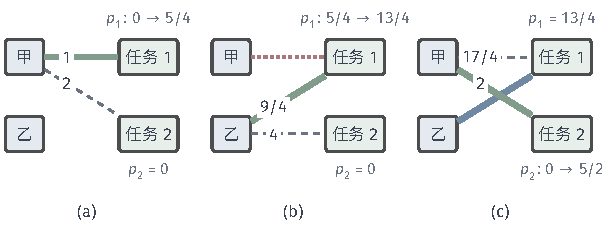
\includegraphics[width=104.122mm]{figures/01-basic-mathematics/04-graphs/tikz/c3-assign-auction/figure.pdf}
  \caption{Auction算法在成本矩阵$\left[\begin{smallmatrix}1&2\\1&4\end{smallmatrix}\right]$上的三次出价，$\varepsilon=1/4$。边旁为出价时的调整成本$c_{i,j}+p_j$，物品旁为价格变化；绿色为本次所得，蓝色为保留的持有，红色点线为被抢走的持有。}
  \label{fig:graph-opt-auction}
\end{figure}

与KM算法相比，Auction算法不要求所选的边恰好紧，只要求每人手中的物品至多比最好选择差$\varepsilon$。这样每一步都只是简单的局部操作，代价是需要说明误差在$r$个竞标者身上怎样累计，以及什么条件下结果仍精确最优\scite{math-graph-bertsekas1991linear}。

\subsubsection{算法流程}

\paragraph{算法状态与初始化}
输入是成本矩阵和$\varepsilon>0$，不算状态。手工竞价的四份记录对应以下状态：
\begin{itemize}
  \item 价格$p_j$：初值全为$0$。
  \item 物品持有者$\mathrm{owner}(j)$与竞标者所得$\sigma(i)$：两套互相对应的记录，初值全为空。
  \item 未指派者队列$Q$：初值含全部竞标者。
\end{itemize}
一次出价可能只是把物品从一人转给另一人，已指派的人数不变，所以停止条件看队列是否为空，而不看已经处理了多少人。每次只处理一名未指派者；最小值并列时取编号最小的物品。

\paragraph{竞价、易主与停止}
从队列取出竞标者$i$后，一次出价分三步：
\begin{itemize}
  \item 比较：扫描第$i$行，计算$q_j=c_{i,j}+p_j$，求最小值$q_{(1)}$及物品$j^\star$，再求$q_{(2)}=\min_{j\neq j^\star}q_j$。不同物品并列时$q_{(2)}=q_{(1)}$，涨价恰为$\varepsilon$。
  \item 涨价：按式~\eqref{eq:graph-opt-auction-bid}令$p_{j^\star}\gets p_{j^\star}+q_{(2)}-q_{(1)}+\varepsilon$。
  \item 易主：若$j^\star$已有持有者$k$，置$\sigma(k)$为空并把$k$放回队列；再置$\mathrm{owner}(j^\star)=i$、$\sigma(i)=j^\star$。物品一旦有了持有者，此后始终有持有者。
\end{itemize}
队列为空时，每个竞标者都持有不同的物品，停止并输出指派$\sigma$、原始成本$C(\sigma)$和最终价格。

\begin{algorithm}[Auction算法]
\label{alg:graph-opt-auction}
输入：$r\geq2$阶有限成本矩阵$\bm C$，$\varepsilon>0$。输出：完整指派$\sigma$、原始成本与价格$\bm p$。
\begin{enumerate}
  \item 置$p_j=0$，$\mathrm{owner}(j)$与$\sigma(i)$全为空，全部竞标者入队$Q$。
  \item 若$Q$为空，转第5步；否则取出$i$，对每个$j$计算$q_j=c_{i,j}+p_j$，求$q_{(1)}=\min_jq_j$及取到它的物品$j^\star$，以及$q_{(2)}=\min_{j\neq j^\star}q_j$。
  \item 置$p_{j^\star}\gets p_{j^\star}+q_{(2)}-q_{(1)}+\varepsilon$。
  \item 若$k=\mathrm{owner}(j^\star)$非空，置$\sigma(k)$为空并把$k$加入$Q$。置$\mathrm{owner}(j^\star)=i$、$\sigma(i)=j^\star$，回到第2步。
  \item 输出$\sigma$、$C(\sigma)=\sum_ic_{i,\sigma(i)}$与$\bm p$。
\end{enumerate}
\end{algorithm}

\paragraph{运行示例}
取$\varepsilon=1/4$，初始队列为甲、乙。三次出价都是伪代码第2—4步的同一循环，见表~\ref{tab:graph-opt-auction-trace}：
\begin{itemize}
  \item 甲：选任务$1$，涨价$2-1+1/4=5/4$。
  \item 乙：选任务$1$，涨价$2$，价格变为$13/4$；甲失去任务$1$，重新入队。
  \item 甲：选任务$2$，涨价$17/4-2+1/4=5/2$，队列变空。
\end{itemize}
最终甲配任务$2$、乙配任务$1$，原始成本为$2+1=3$。最终价格不是原问题的额外支出。

再逐人核对$\varepsilon$条件。甲手中物品的调整成本与当前最好选择分别为
\[
  2+\tfrac52=\tfrac92,\qquad \min\bigl\{\tfrac{17}4,\tfrac92\bigr\}=\tfrac{17}4,
\]
恰好差$1/4$。乙手中的任务$1$调整成本为$17/4$，另一项为$4+5/2=13/2$，乙持有的就是最好选择。

\begin{table}[!htb]
  \centering\small
  \caption{Auction算法在成本矩阵$\left[\begin{smallmatrix}1&2\\1&4\end{smallmatrix}\right]$上的出价，$\varepsilon=1/4$。比较值为出价时的$c_{i,j}+p_j$；价格与持有者为出价后的状态。}
  \label{tab:graph-opt-auction-trace}
  \begin{tabular}{@{}llllll@{}}
    \toprule
    出价者 & 比较值 & 所选 & 涨价 & 价格$\bm p$ & 持有者 \\
    \midrule
    甲 & $1$，$2$ & 任务$1$ & $5/4$ & $(5/4,0)$ & 甲，— \\
    乙 & $9/4$，$4$ & 任务$1$ & $2$ & $(13/4,0)$ & 乙，— \\
    甲 & $17/4$，$2$ & 任务$2$ & $5/2$ & $(13/4,5/2)$ & 乙，甲 \\
    \bottomrule
  \end{tabular}
\end{table}

\subsubsection{正确性与复杂度}

运行示例结束时，甲的选择比最好选择差$1/4$，乙没有差额。把这项性质一般化，就是算法维护的条件。

\begin{definition}[$\varepsilon$互补松弛]
\label{def:graph-opt-eps-cs}
设$\varepsilon\geq0$，$\bm p$为价格，$\sigma$为部分或完整指派。若每个已指派的竞标者$i$都满足
\begin{equation}
  c_{i,\sigma(i)}+p_{\sigma(i)}\leq\min_{j}\bigl(c_{i,j}+p_j\bigr)+\varepsilon,
  \label{eq:graph-opt-eps-cs}
\end{equation}
就称$(\sigma,\bm p)$满足\term{$\varepsilon$互补松弛}（$\varepsilon$-complementary slackness）。
\end{definition}

$\varepsilon=0$时，它就是“匹配边是紧边”的价格写法，下面的定理说明这一对应。

\begin{lemma}[$\varepsilon$互补松弛的保持]
初始状态满足$\varepsilon$互补松弛，此后每次出价都保持它。
\end{lemma}

\begin{proof}
初始时没有人被指派，条件自动成立。考虑竞标者$i$对$j^\star$的一次出价。对新持有者$i$，涨价后$c_{i,j^\star}+p_{j^\star}=q_{(2)}+\varepsilon$，而其他物品的调整成本都不小于$q_{(2)}$，$j^\star$本身的调整成本也不小于$q_{(2)}+\varepsilon$，所以条件成立。对其他仍持有物品的竞标者$k$，只有$p_{j^\star}$变了，而$k$持有的不是$j^\star$：$k$手中物品的调整成本不变，右端的最小值不会下降，条件继续成立。失去$j^\star$的人回到未指派状态，不受条件约束。
\end{proof}

\begin{theorem}[Auction算法的误差界]
\label{thm:graph-opt-auction}
设成本矩阵完整有限，Auction算法以完整指派$\sigma$和价格$\bm p$停止，$C^\star$为最优指派成本。则
\begin{equation}
  0\leq C(\sigma)-C^\star\leq r\varepsilon.
  \label{eq:graph-opt-auction-error}
\end{equation}
若全部成本为整数且$0<\varepsilon<1/r$，则$\sigma$是最优指派。
\end{theorem}

\begin{proof}
令$u_i=\min_j(c_{i,j}+p_j)$、$v_j=-p_j$。对任意$i,j$有$u_i\leq c_{i,j}+p_j$，即$u_i+v_j\leq c_{i,j}$，所以$(\bm u,\bm v)$是可行标号，由第~\ref{sec:graph-opt-assign-labels}小节，$\sum_iu_i+\sum_jv_j\leq C^\star$。

由$\varepsilon$互补松弛，
\[
  c_{i,\sigma(i)}\leq u_i-p_{\sigma(i)}+\varepsilon=u_i+v_{\sigma(i)}+\varepsilon,
\]
即每条匹配边的剩余量至多为$\varepsilon$。对$i$求和，$\sigma$是置换，每个$v_j$恰出现一次，
\[
  C(\sigma)\leq\sum_iu_i+\sum_jv_j+r\varepsilon\leq C^\star+r\varepsilon.
\]
$C(\sigma)\geq C^\star$是最优值的定义。成本为整数时，$C(\sigma)-C^\star$是小于$r\varepsilon<1$的非负整数，只能为$0$。
\end{proof}

一般的实数成本在固定的正$\varepsilon$下只有这个误差界。两人例中$r\varepsilon=1/2<1$，成本为整数，所以得到的成本$3$精确最优。

有限终止要用到“完整有限成本”和“零初始价格”。记成本范围为
\[
  \Delta=\max_{i,j}c_{i,j}-\min_{i,j}c_{i,j}.
\]
物品一旦被出价就始终有持有者，已持有物品的数目等于已指派的人数；只要还没停止，就至少有一个物品从未被出价，价格仍为$0$。

竞标者$i$对$j^\star$出价时，若另有从未被出价的物品$j_0\neq j^\star$，则$q_{(2)}\leq c_{i,j_0}$，涨价后
\[
  p_{j^\star}=q_{(2)}+\varepsilon-c_{i,j^\star}\leq c_{i,j_0}-c_{i,j^\star}+\varepsilon\leq\Delta+\varepsilon.
\]
若没有这样的$j_0$，$j^\star$就是最后一个未被出价的物品，这次出价后人人都有物品，算法停止。

每次出价至少涨价$\varepsilon$，同一物品被出价$k$次后价格至少为$k\varepsilon$，所以除停止前的最后一次外，每个物品至多被出价$\Delta/\varepsilon+1$次，总出价次数
\begin{equation}
  B\leq r\bigl(\Delta/\varepsilon+1\bigr)+1.
  \label{eq:graph-opt-auction-bids}
\end{equation}
这个论证依赖每个物品都可选：禁配实例若不可行，价格可以无限上涨而永不停止。

按总出价次数$B$分析稠密实现：每次出价扫描一行为$O(r)$，读入矩阵为$O(r^2)$，总时间$O(r^2+rB)$；价格、持有者、指派与队列为$O(r)$，成本表另占$O(r^2)$。

由上面的界，整数成本且取$\varepsilon=1/(r+1)$时，$B=O(r^2\Delta)$，总时间为$O(r^3\Delta)$，随成本范围增长，不能把KM算法的$O(r^3)$直接套用到Auction算法上。$\varepsilon$越小，误差界越紧，但需要的出价可能越多；更强的复杂度界依赖下一小节的缩放策略\scite{math-graph-bertsekas2025auction-ch2}。

\subsubsection{误差缩放与适用边界}

固定一个很小的$\varepsilon$，开始阶段价格从零慢慢上涨，许多出价只是一点点地挪动价格。\term{$\varepsilon$缩放}（$\varepsilon$-scaling）先用较大的$\varepsilon$完成一个较粗的指派，得到大致合理的价格，再逐阶段缩小$\varepsilon$，并把上一阶段的价格作为下一阶段的初值。

最简单的做法是每阶段保留价格、清空指派、全部竞标者重新入队竞价；若想保留部分配对，须先解除不满足新$\varepsilon$条件的配对再继续。只缩小参数而保留完整指派是错误的：队列已空，算法会直接停止，新的$\varepsilon$条件根本没有被检查。最后一阶段的$\varepsilon$按定理~\ref{thm:graph-opt-auction}的要求选取\scite{math-graph-bertsekas2024auction}。

非方阵、未分配惩罚等情形，先按第~\ref{sec:graph-opt-assign-rectangular}小节补成方阵。允许边不完整时，竞标者只在自己的允许物品中比较，这时要先用第~\ref{sec:graph-opt-match-algorithm}小节的方法确认存在完美匹配，因为基本算法不会自行识别不可行。

只有一个允许物品的行，排除最好选择后没有次好值，涨价公式无法使用；这样的行在任何完整指派中都只能配这个物品，可以先把这一对固定下来，删去相应的行和列。不能把不存在的次好值当成$+\infty$代入公式，那会让价格变成无穷。

浮点实现中，涨价、并列判断和$\varepsilon$条件都受舍入影响，$\varepsilon$很小时涨价可能被舍入吞掉一部分。整数成本下“$\varepsilon<1/r$即精确最优”的结论，要求算术精度足以区分相差$\varepsilon$的值。Auction算法另有并行与异步版本，多名竞标者同时出价时须处理冲突；它们的复杂度结论不适用于本节的串行版本。

\subsection{方法比较与结果检验}
\label{sec:graph-opt-assign-analysis}

两种算法解同一个方阵指派。KM算法保持可行标号、只在紧边上增广，结束时给出精确证书，可直接处理禁配，稠密方阵上为$O(r^3)$。Auction算法维护价格和满足$\varepsilon$互补松弛的部分指派，每步一次出价和易主；其保证随$\varepsilon$、成本整数性和算术精度而定，出价次数随成本范围与$\varepsilon$变化，比较前须先说明这些条件。

检验指派先看原始问题的可行性：每个真实对象按模型要求配对或计入惩罚，所用的列互不相同，全部配对都是允许边；再按原始成本重算总成本。

KM算法的结果还要检查证书：对全部允许边验证$u_i+v_j\leq c_{i,j}$，对所选的边验证取等号，并核对总成本等于$\sum_iu_i+\sum_jv_j$。在两人例中，四条边的剩余量依次为$0,0,0,2$，所选的甲—$2$、乙—$1$剩余量为零，成本与下界同为$3$。

Auction算法的结果检查最终价格下每人的$\varepsilon$互补松弛，再由定理~\ref{thm:graph-opt-auction}给出目标误差界；只有在整数成本与$\varepsilon<1/r$等条件下才能称为精确最优。浮点实现中，可行性、紧性和出价比较都只能在容差内判断，应说明所用容差，不把近似相等当成精确证书。

标号和价格都在为配对成本提供可以核查的界：可行标号直接给出下界，价格经$u_i=\min_j(c_{i,j}+p_j)$、$v_j=-p_j$转成同样的下界。第~\ref{sec:graph-min-cost-flow}章把这种给顶点配数的做法推广到一般容量与供需网络上的节点势；指派也能写成那里的特例，但统一的模型并不意味着必须选用相同的算法。

% 第6章：本章小结。
\FloatBarrier
\section{本章小结}
\label{sec:matching-assignment-summary}

本章开头区分了两种要求：只求配对最多，或要求每个对象都配上并使总成本最低。对第一种，二部图匹配与单位容量网络上的整数流一一对应，残量增广路径落到二部图上就是交替路径，于是匹配最大当且仅当不存在增广路径。这个判据比“不能再加边”强：极大匹配可能仍有增广路径，改进要允许中间顶点换伙伴。匈牙利算法只维护伙伴数组，逐个左侧顶点用深度优先搜索找增广路径，总时间$O(n+pm)$，其中$p$为较小一侧的顶点数；Hopcroft--Karp算法按层成批增广，得到$O(n+m\sqrt n)$。这些构造都依赖给定的两侧划分，不能直接用于含奇数长环的一般图。

对第二种，可行标号给出全部完整指派的共同下界，只用紧边的完美匹配达到这个下界，因而最优。KM算法在紧边上生长交替树，受阻时按最小松弛量调标，使下界升高、树继续生长；结束时匹配与标号构成精确证书，禁配也能直接处理，稠密方阵上为$O(r^3)$。Auction算法用价格协调争抢，维护$\varepsilon$互补松弛：最终指派的成本至多比最优值高$r\varepsilon$，只有在整数成本且$\varepsilon<1/r$时才保证精确最优；出价次数随成本范围与$\varepsilon$变化，总时间为$O(r^2+rB)$。

两类结果的核对方式也不同。最大匹配用单位容量网络中与配对数同值的割核对；KM算法的结果逐边核对标号可行与所选边取等号；Auction算法的结果只能核对最终价格下的$\varepsilon$条件，再据此给出误差界。矩形、禁配与允许不配对的情形，都要先补成方阵并把惩罚写进成本，求解后按原始成本重算。

标号和价格都是给顶点配上的数，用来为配对成本提供可核查的界：价格经$u_i=\min_j(c_{i,j}+p_j)$、$v_j=-p_j$就转成可行标号。下一章把这种做法推广为一般容量与供需网络上的节点势，最大流、匹配与指派也都能写成那里的最小费用流。


% 第7章：最小费用流（问题；最优性条件；网络单纯形法；统一表示；结果检验）。

\chapter{最小费用流}
\label{sec:graph-min-cost-flow}
\label{chap:min-cost-flow}

第~\ref{sec:graph-max-flow}章只问能送多少。实际调运中，各处的产量与需求事先给定，各条线路运价不同，要比较的是满足供需的方案中哪个总费用最低。本章回答三个问题：怎样把容量、供需和单位费用写进同一个模型；怎样判断一个方案已经最省；怎样从一个可行方案出发逐步改进到最优。

第~\ref{sec:graph-opt-mcf-problem}节给出模型，并说明下界、供需平衡与可行性怎样处理。第~\ref{sec:graph-opt-mcf-optimality}节回答最优性：对方案的任何改动都可以看成沿一个环把货物改道，所以有省钱的环，当前方案就不是最优；没有，就是最优。在第~\ref{sec:graph-opt-residual-network}节的残量网络上给每条残量弧配上费用，这一观察就成为负费用环判据；再借第~\ref{chap:shortest-paths}章的最短距离构造节点势，判据化为逐弧可查的证书。

第~\ref{sec:graph-opt-network-simplex}节的\term{网络单纯形法}（network simplex method，亦称网络单形法）把方案记在一棵生成树上，每次只沿一个环改道。它是线性规划单纯形法在网络上的特例，这里只用树、环和守恒式建立它，不依赖一般的线性规划理论。第~\ref{sec:graph-opt-mcf-unified}节把最大流、二部图匹配和指派写成最小费用流，第~\ref{sec:graph-opt-ns-analysis}节说明怎样回到原始问题核对结果，第~\ref{sec:graph-opt-mcf-other-methods}节简述沿同一残量结构组织改进的其他算法。

本章为了把字母$c$留给费用，把容量改记为上界$u_{i,j}$，弧写作$(i,j)$或$i\to j$；顶点数仍为$n$，弧数仍为$a$。

\section{最小费用流问题}
\label{sec:graph-opt-mcf-problem}

设想几个仓库经中转站向几家商店供货：库存要全部运出，需求要恰好满足；每条线路有运量上限，有些按合同还有最低运量，每运一单位付相应的运价。把各处看成顶点、线路看成有向弧，就得到下面的问题。

\begin{definition}[最小费用流问题]
\label{def:graph-opt-min-cost-flow}
设$\mathcal G=(V,E)$是有限有向图，每个顶点$i$有供需量$b_i\in\mathbb R$，每条弧$(i,j)\in E$有有限的下界$\ell_{i,j}$、上界$u_{i,j}$（$\ell_{i,j}\leq u_{i,j}$）与单位费用$c_{i,j}\in\mathbb R$。给每条弧赋一个流量$x_{i,j}$，若向量$\bm x$满足
\begin{equation}
\begin{gathered}
  \sum_{j:\,(i,j)\in E}x_{i,j}-\sum_{j:\,(j,i)\in E}x_{j,i}=b_i\quad(i\in V),\\
  \ell_{i,j}\leq x_{i,j}\leq u_{i,j}\quad((i,j)\in E),
\end{gathered}
  \label{eq:graph-opt-mcf-constraints}
\end{equation}
则称$\bm x$为可行流。\term{最小费用流}（minimum-cost flow）问题是在全部可行流中最小化总费用
\begin{equation}
  \bm c^{\top}\bm x=\sum_{(i,j)\in E}c_{i,j}x_{i,j}.
  \label{eq:graph-opt-mcf-cost}
\end{equation}
\end{definition}

守恒式左边是顶点$i$的净流出，所以$b_i>0$表示$i$是供给点，要净送出$b_i$单位；$b_i<0$表示需求点，要净收进$-b_i$单位；$b_i=0$的顶点只做中转。把全部守恒式相加，每条弧的流量正负各计一次，左边为零，所以$\sum_{i\in V}b_i=0$是可行流存在的必要条件。

它不充分：平衡的供需不保证有路可走、容量够用。图~\ref{fig:graph-opt-mcf-network}的网络中，若把$s\to a$与$s\to t$的容量都改成$1$，从$s$出发的总容量只有$2$，供需虽然平衡，问题却没有可行流。

\begin{figure}[!htb]
  \centering
  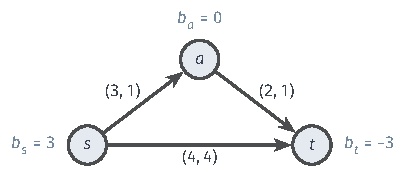
\includegraphics[width=68.527mm]{figures/01-basic-mathematics/04-graphs/tikz/c3-mcf-network/figure.pdf}
  \caption{三点最小费用流算例。$s$供给$3$单位，$t$需求$3$单位，$a$只做中转；弧旁括号依次为容量与单位费用，下界均为$0$。绕行$s\to a\to t$的单位费用为$2$，低于直达弧的$4$，但绕行量受$a\to t$的容量$2$限制。}
  \label{fig:graph-opt-mcf-network}
\end{figure}

按弧序$s\to a$、$a\to t$、$s\to t$把流量写成向量。$3$单位全走直达弧是$(0,0,3)$，让$2$单位绕行、$1$单位直达是$(2,2,1)$，两者的费用分别为
\[
  \begin{aligned}
    (0,0,3)&:\quad 3\times4=12,\\
    (2,2,1)&:\quad 2\times(1+1)+1\times4=8.
  \end{aligned}
\]
后面将证明$8$就是最小费用。

正下界（如合同规定的最低运量）的处理办法是先把下界部分“预先送出”，再对剩余部分求解。令
\[
  x_{i,j}=\ell_{i,j}+y_{i,j},\qquad 0\leq y_{i,j}\leq u_{i,j}-\ell_{i,j}.
\]
预先送出的下界流量已经使顶点$i$净流出$\sum_j\ell_{i,j}-\sum_j\ell_{j,i}$，所以$\bm y$应满足的剩余供需为
\begin{equation}
  b'_i=b_i-\sum_{j:\,(i,j)\in E}\ell_{i,j}+\sum_{j:\,(j,i)\in E}\ell_{j,i}.
  \label{eq:graph-opt-mcf-shifted-supply}
\end{equation}
目标变为$\sum c_{i,j}y_{i,j}+\bm c^{\top}\bm\ell$，后一项是常数。两个问题的可行解与最优解通过$\bm x=\bm\ell+\bm y$一一对应。

图~\ref{fig:graph-opt-mcf-lower-bound}把三点网络中$s\to t$的下界改为$1$：这条弧的容量从$4$变为$3$，$s$的剩余供给从$3$降为$2$，$t$的剩余需求从$3$降为$2$，目标另加常数$c_{s,t}\ell_{s,t}=4$。只改容量而不改供需，下界那一单位就被重复计算。

新问题的最优解是$\bm y=(2,2,0)$，费用$4$；加回下界与常数，得到原问题的最优流$\bm x=(2,2,1)$与费用$8$。

上下界相等的固定弧平移后容量为零，可以先删去，只保留它对供需和常数的贡献。以下除非特别说明，都假定下界已平移为零、固定弧已删去。

\begin{figure}[!htb]
  \centering
  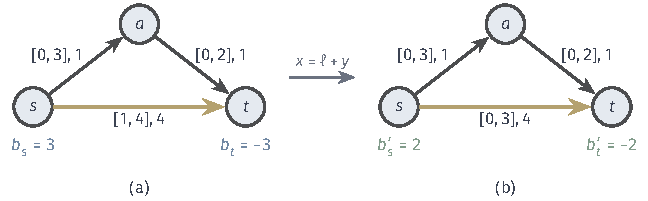
\includegraphics[width=109.767mm]{figures/01-basic-mathematics/04-graphs/tikz/c3-mcf-lower-bound-shift/figure.pdf}
  \caption{下界平移。(a)中黄色弧$s\to t$的流量须在$[1,4]$内，弧旁依次为流量区间与单位费用。(b)令$x=\ell+y$后，该弧的区间变为$[0,3]$，$s$与$t$的供需同时各减少$1$单位（绿色），目标另加常数$4$。}
  \label{fig:graph-opt-mcf-lower-bound}
\end{figure}

从源点$s$向汇点$t$输送固定量$F$时，令$b_s=F$、$b_t=-F$，其余$b_i=0$。全部$b_i=0$时的可行流称为\term{循环流}（circulation）；第~\ref{sec:graph-opt-mcf-unified}节会用它表达最大流。

先尽量多送、再在全部最大流中挑费用最低的，称为\term{最小费用最大流}（minimum-cost maximum flow）：先用第~\ref{sec:graph-max-flow}章的方法求出最大流值$v^\star$，再取$F=v^\star$。

在有限上下界下，可行流集合是$\mathbb R^{a}$中的闭有界集（$a=|E|$），总费用是线性函数，而闭有界集上的连续函数必能取到最小值（多元极值定理，可参考\BookChapterRef{chap:normed-inner-product-spaces}{第~\ref{chap:normed-inner-product-spaces}章}），所以只要可行流存在，最小费用一定能取到；可行性由后文网络单纯形法的第一阶段判断。

若允许无穷容量，可无限推送的负费用环使费用没有下界；本章主线只讨论有限容量，无穷容量放在第~\ref{sec:graph-opt-ns-improvements}小节。

\section{费用残量网络与最优性条件}
\label{sec:graph-opt-mcf-optimality}

判断最优不能逐一比较全部可行流。这里沿用第~\ref{sec:graph-opt-residual-network}节的残量网络描述流量还能怎样改，只是每条残量弧多带一个费用。

给定可行流$\bm x$。对每条原弧$(i,j)$，若$x_{i,j}<u_{i,j}$，建立正向残量弧$i\to j$，剩余容量$u_{i,j}-x_{i,j}$，费用$c_{i,j}$；若$x_{i,j}>\ell_{i,j}$，建立反向残量弧$j\to i$，剩余容量$x_{i,j}-\ell_{i,j}$，费用$-c_{i,j}$，表示撤回一单位省下$c_{i,j}$。原网络同时有$i\to j$与$j\to i$两条弧时，各自的残量弧要记住来自哪条原弧，不能合并。

改道在残量网络中就是一个环。图~\ref{fig:graph-opt-mcf-residual-cycle}从全走直达的流$(0,0,3)$出发：把一单位改走中转，要在$s\to a$、$a\to t$各加一单位，并从直达弧撤回一单位，三步首尾相接成残量环$s\to a\to t\to s$，费用为
\[
  c_{s,a}+c_{a,t}-c_{s,t}=1+1-4=-2.
\]
逐点看，$s$、$a$、$t$各自少走一条弧、多走一条弧，净流出不变。

逐边看，$s\to a$还能加$3$，$a\to t$还能加$2$，直达弧还能撤回$3$，所以最多改道
\[
  \min\{3,2,3\}=2
\]
单位，费用从$12$降为$8$。

\begin{figure}[!htb]
  \centering
  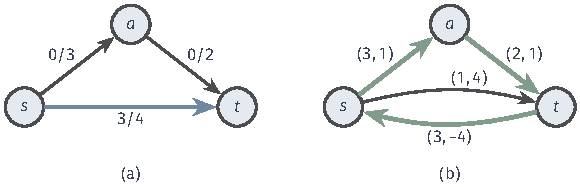
\includegraphics[width=103.579mm]{figures/01-basic-mathematics/04-graphs/tikz/c3-mcf-residual-cycle/figure.pdf}
  \caption{残量网络中的负费用环。(a)全部$3$单位走直达弧的可行流，弧旁为流量与容量。(b)它的残量网络，弧旁为剩余容量与费用；直达弧产生可追加$1$单位的正向弧和可撤回$3$单位、费用$-4$的反向弧$t\to s$。绿色环费用$-2$，推送$2$单位使费用降$4$。}
  \label{fig:graph-opt-mcf-residual-cycle}
\end{figure}

一般地，沿残量网络中的有向环$C$推送$\theta>0$单位，是指正向残量弧对应的原弧流量加$\theta$，反向残量弧对应的原弧流量减$\theta$。环上每个顶点恰有一条环弧进入、一条离开，净流出不变；$\theta$不超过环上的最小剩余容量时，上下界仍然满足。

推送后费用改变$\theta\,c(C)$，其中$c(C)$是环上残量费用之和。所以有$c(C)<0$的环时当前流不是最优。反过来也成立，关键是任何可行流与当前流之差都能拆成残量环的叠加。

\begin{theorem}[负费用环判据]
\label{thm:graph-opt-negative-cycle}
可行流$\bm x$是最小费用流，当且仅当它的残量网络中不存在费用为负的有向环。
\end{theorem}

\begin{proof}
必要性已由上面的推送论证给出，下证充分性。任取可行流$\bm x'$，令$\bm d=\bm x'-\bm x$。两个流满足同一组供需，所以$\bm d$在每个顶点的净流出为零。

逐条考察原弧$(i,j)$：若$d_{i,j}>0$，则$x_{i,j}<x'_{i,j}\leq u_{i,j}$，正向残量弧存在且剩余容量至少为$d_{i,j}$，在它上面放$d_{i,j}$；若$d_{i,j}<0$，则$x_{i,j}>x'_{i,j}\geq\ell_{i,j}$，反向残量弧存在，在它上面放$-d_{i,j}$。这样得到残量弧上的一组非负数$\bm g$，它在每个顶点流入等于流出，按残量费用加权的总和等于$\bm c^{\top}\bm x'-\bm c^{\top}\bm x$。

若$\bm g\neq\bm 0$，从任一取正值的残量弧出发，沿正值弧前进：每到达一个顶点，它的流入为正，必有一条正值出弧可走。顶点有限，前进中必然回到某个走过的顶点，截出一个有向环$C_1$。令$\lambda_1>0$为$\bm g$在$C_1$上的最小值，从环上各弧减去$\lambda_1$，剩余部分仍非负且守恒，而取正值的弧至少少了一条。重复有限次，得到
\[
  \bm c^{\top}\bm x'-\bm c^{\top}\bm x=\sum_k\lambda_k\,c(C_k),\qquad\lambda_k>0.
\]
每个$C_k$都由残量弧组成。残量网络中没有负费用环时，右边每项非负，$\bm x'$不比$\bm x$便宜。
\end{proof}

这个判据本身还不是算法，也不断言最优流唯一。直接逐个检查残量网络中的环也行不通，因为环的个数可能随规模指数增长。为了把条件改成逐弧检查，给每个顶点$i$配一个实数$\pi_i$，称为\term{节点势}（node potential），并定义弧$(i,j)$的\term{约化费用}（reduced cost）
\begin{equation}
  \bar c_{i,j}=c_{i,j}-\pi_i+\pi_j.
  \label{eq:graph-opt-reduced-cost}
\end{equation}
残量弧使用同一公式：反向残量弧$j\to i$的费用为$-c_{i,j}$，约化费用为
\[
  -c_{i,j}-\pi_j+\pi_i=-\bar c_{i,j}.
\]

沿有向环相加时，每个顶点的势在出弧上以$-\pi$、在入弧上以$+\pi$各出现一次，相消，所以环的约化费用等于原费用。因此，若能找到一组势，使所有残量弧的约化费用都非负，残量网络就没有负费用环。

反过来，残量网络没有负费用环时，这样的势一定存在。加入虚拟顶点$r$，向每个顶点连一条零费用弧；新图的环不经过$r$，仍无负环。记$d_i$为$r$到$i$的最短路径费用，绕环不会更便宜，只需比较有限条简单路径，所以$d_i$有限。

对残量弧$i\to j$及其费用$c'$，到$i$的最短路径接上这条弧是一条到$j$的行走，去掉其中的环不增加费用，所以$d_j\leq d_i+c'$。取$\pi_i=-d_i$，即得
\[
  c'-\pi_i+\pi_j=c'+d_i-d_j\geq0.
\]
实际可用第~\ref{sec:graph-opt-bellman-ford}节的Bellman--Ford算法求$d_i$，它报告负环时就找到了可推送的负费用环。

势可以理解为各顶点上货物的“边际运费”。把$\pi_i$看成从$i$再送一单位到需求点$t$的最低费用（$\pi_t=0$），允许借助残量弧撤回已有流量。图~\ref{fig:graph-opt-mcf-potentials}以流$(2,2,1)$为例：从$s$再送一单位，绕行已被$a\to t$卡住，只能直达，$\pi_s=4$。

从$a$再送一单位，最便宜的是让一单位原本经$a$绕行的货改走直达，$a$处这单位顶替它前往$t$，省$1$付$4$，$\pi_a=3$。这正是由最短距离构造的势。

\begin{figure*}[!htb]
  \centering
  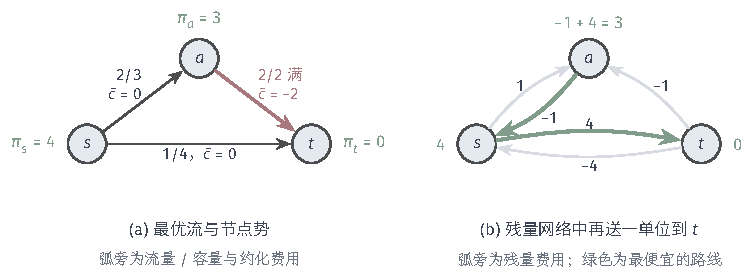
\includegraphics[width=127.593mm]{figures/01-basic-mathematics/04-graphs/tikz/c3-mcf-potentials/figure.pdf}
  \caption{节点势的直观含义。(a)流$(2,2,1)$与势$(4,3,0)$；界内弧约化费用为零，满载弧$a\to t$为$-2$（红色）。(b)残量网络，弧旁为残量费用；绿色为从各顶点再送一单位到$t$的最便宜路线，费用$4$与$3$即$\pi_s,\pi_a$。}
  \label{fig:graph-opt-mcf-potentials}
\end{figure*}

按这种理解，约化费用$\bar c_{i,j}=c_{i,j}+\pi_j-\pi_i$比较两种送货方式：经弧$(i,j)$送出一单位，付$c_{i,j}$再付$\pi_j$；或按$i$现行的边际方式送出，付$\pi_i$。$\bar c_{i,j}<0$表示这条弧更便宜，应当多用；$\bar c_{i,j}>0$表示更贵，应当少用。最优流中能加量的弧不能更便宜，能减量的弧不能更贵。

“全部残量弧约化费用非负”于是逐弧翻译为：弧在下界时只有正向残量弧，要求$\bar c_{i,j}\geq0$；在上界时只有反向残量弧，要求$\bar c_{i,j}\leq0$；严格在两界之间时两条都存在，要求$\bar c_{i,j}=0$。

\begin{theorem}[节点势最优性证书]
\label{thm:graph-opt-potential-certificate}
设固定弧已删去，$\bm x$是可行流，$\bm\pi$是一组节点势。若对每条弧$(i,j)$都有
\begin{equation}
  \bar c_{i,j}\ \begin{cases}
    \geq0, & x_{i,j}=\ell_{i,j},\\
    \leq0, & x_{i,j}=u_{i,j},\\
    =0, & \ell_{i,j}<x_{i,j}<u_{i,j},
  \end{cases}
  \label{eq:graph-opt-mcf-certificate}
\end{equation}
则$\bm x$是最小费用流。
\end{theorem}

\begin{proof}
任取可行流$\bm x'$。把$c_{i,j}=\bar c_{i,j}+\pi_i-\pi_j$代入费用差，
\[
  \begin{aligned}
    \bm c^{\top}(\bm x'-\bm x)
    &=\sum_{(i,j)\in E}\bar c_{i,j}(x'_{i,j}-x_{i,j})\\
    &\quad+\sum_{(i,j)\in E}(\pi_i-\pi_j)(x'_{i,j}-x_{i,j}).
  \end{aligned}
\]
第二个和按顶点归组，等于对每个$i$把$\pi_i$乘以顶点$i$在$\bm x'$与$\bm x$下净流出之差再求和；两个流满足同一组供需，这些差全为零。

第一个和逐项非负：若$x_{i,j}=\ell_{i,j}$，则$x'_{i,j}-x_{i,j}\geq0$且$\bar c_{i,j}\geq0$；若$x_{i,j}=u_{i,j}$，则$x'_{i,j}-x_{i,j}\leq0$且$\bar c_{i,j}\leq0$；其余情形$\bar c_{i,j}=0$。所以$\bm c^{\top}\bm x'\geq\bm c^{\top}\bm x$。
\end{proof}

删去固定弧是为了避免$\ell_{i,j}=u_{i,j}$时前两个条件同时出现。这组条件在线性规划中称为互补松弛条件。

流量与势合起来构成证书：核对可行性和每条弧上的一个符号，就能确认最优，不必相信求解过程。

在三点网络中取流$(2,2,1)$与势$(4,3,0)$，三条弧的约化费用为
\[
  \bar c_{s,a}=1-4+3=0,\quad\bar c_{s,t}=4-4+0=0,\quad\bar c_{a,t}=1-3+0=-2.
\]
界内的两条弧$s\to a$、$s\to t$的约化费用都是零，上界弧$a\to t$的约化费用为$-2\leq0$，所以费用$8$最小。

\section{网络单纯形法}
\label{sec:graph-opt-network-simplex}

网络单纯形法把当前流记在一棵生成树上，用不在树上的弧的约化费用寻找改进方向，再沿相应的环调整流量。下面先在三点网络上说明这些做法。

\subsection{主要思想}

第~\ref{sec:graph-opt-mcf-optimality}节把三点网络的改道写成了负费用环$s\to a\to t\to s$：每改道一单位省$2$，最多改$2$单位，费用$12\to8$。负环指明了改进方向，剩下的问题是有组织地找到它们：记录当前流的方式应使候选的环容易列出，环的费用和改道量容易算出。

办法是把流记在一棵树上。规定$s\to a$的流量固定为$0$，只让$s\to t$与$a\to t$待定：中转点$a$没有外部供需，所以$a\to t=0$；$t$要收的$3$单位只能来自$s\to t$，所以$s\to t=3$。固定一部分弧后，其余流量顺着树由守恒式算出。

一般地，忽略方向后构成生成树的弧集记为$T$，称为树弧；其余弧的流量固定在下界或上界，分别组成$L$与$U$。三元组$(T,L,U)$称为一个\term{树基}（spanning tree basis）。

叶子只关联一条树弧，它的守恒式中其余各项已知，于是解出这条树弧的流量；删去叶子再重复，就求出全部树弧流量。若它们都在上下界内，称$(T,L,U)$为可行树基。

把$s\to a$加进树，恰好多出一个环，正是上面的改道环。一般地，非树弧与树上连接其两端的唯一路径合成的环称为\term{基本环}（fundamental cycle）。沿这个环推送$2$单位后，$a\to t$到达上界，它退出树、进入$U$，$s\to a$进入树。这一步称为换基：它同时更新了表示当前流的树，使新流$(2,2,1)$仍由新树确定。

只在树形方案中寻找，不会错过最优解。若严格位于两界之间的弧含有一个环，沿环的两个方向都能推送少量流量，两方向单位费用变化互为相反数，至少一个方向不增加费用；沿它推到某条弧碰界，环就被打断。反复这样做，界内弧不再含环，补上一些在界上的弧即成生成树。

图~\ref{fig:graph-opt-ns-why-tree}中，流$(1,1,2)$的三条弧都在界内而成环，推送$1$单位后$a\to t$满载，得到$(2,2,1)$，环被打断。树形方案只有有限多个。

\begin{figure*}[!htb]
  \centering
  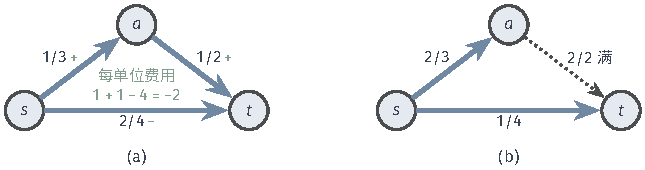
\includegraphics[width=113.249mm]{figures/01-basic-mathematics/04-graphs/tikz/c3-ns-why-tree/figure.pdf}
  \caption{打断界内弧的环。(a)流$(1,1,2)$的三条弧都在界内，按绿色符号沿环推送，每单位费用变化$-2$。(b)推送$1$单位后$a\to t$到上界，界内弧不再成环，费用由$10$降为$8$。}
  \label{fig:graph-opt-ns-why-tree}
\end{figure*}

同一棵树还给出节点势。令$\pi_t=0$，要求两条树弧约化费用为零，得$\pi_s=4$、$\pi_a=1$。候选弧$s\to a$的约化费用
\[
  \bar c_{s,a}=1-4+1=-2
\]
恰是每改道一单位的费用变化。

这不是巧合：把基本环上每个$c$换成$\bar c+\pi_i-\pi_j$，势相消，树弧约化费用为零，只剩非树弧自己的约化费用。所以定价，即检查非树弧约化费用的符号，就是逐个评估全部基本环。

树上的路径可能逆着原弧方向走，$\pi_i-\pi_j$是沿树从$i$到$j$的有符号费用，顺弧计正、逆弧计负。它一般不是全图中的最短距离：第~\ref{sec:graph-opt-mcf-optimality}节把势解释为“边际运费”，是针对最优流说的。

概括起来，网络单纯形法只做三件事：只在树形方案中寻找；用一棵树同时决定流和势；每次找一条约化费用符号不对的非树弧，沿它的基本环改道，改到某条弧碰界为止，再让这条弧离开树。图~\ref{fig:graph-opt-ns-loop}画出了这个循环，系统的讲述可参考Bertsekas的网络优化教材\scite{math-graph-bertsekas1998network}。

\begin{figure*}[!htb]
  \centering
  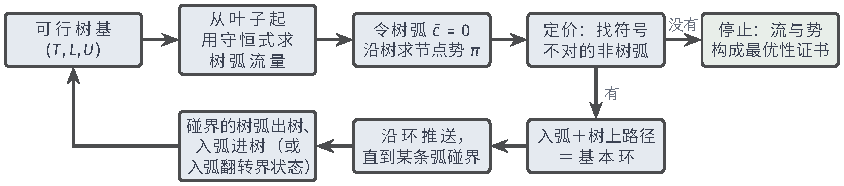
\includegraphics[width=142.762mm]{figures/01-basic-mathematics/04-graphs/tikz/c3-ns-loop/figure.pdf}
  \caption{网络单纯形法的一轮。定价后若无符号不对的非树弧就停止，否则沿基本环推送到某弧碰界：碰界的树弧出树、入弧进树，或入弧自身翻转界状态。}
  \label{fig:graph-opt-ns-loop}
\end{figure*}

\subsection{算法流程}

\paragraph{算法状态}
手算用到的记录——每条弧送多少、哪些弧成树、其余弧停在哪个界、各点势多少——列在表~\ref{tab:graph-opt-ns-state}中，并以$t$为根记下每个顶点的父顶点、父边与深度。父顶点和父边用于沿树找路，深度帮助入弧两端回溯到公共祖先。

\begin{table}[!htb]
  \centering\small
  \caption{三点网络在树$T=\{s\to t,a\to t\}$下的状态，根为$t$。左表为弧记录，右表为顶点记录。}
  \label{tab:graph-opt-ns-state}
  \begin{tabular}{@{}lcccc@{}}
    \toprule
    弧 & 流量 & 界 & 费用 & 状态 \\
    \midrule
    $s\to a$ & $0$ & $[0,3]$ & $1$ & $L$ \\
    $a\to t$ & $0$ & $[0,2]$ & $1$ & $T$ \\
    $s\to t$ & $3$ & $[0,4]$ & $4$ & $T$ \\
    \bottomrule
  \end{tabular}\quad
  \begin{tabular}{@{}lcccc@{}}
    \toprule
    顶点 & 势 & 父顶点 & 父边 & 深度 \\
    \midrule
    $s$ & $4$ & $t$ & $s\to t$ & $1$ \\
    $a$ & $1$ & $t$ & $a\to t$ & $1$ \\
    $t$ & $0$ & — & — & $0$ \\
    \bottomrule
  \end{tabular}
\end{table}

平移下界、删去固定弧后的网络及其邻接结构在开始前构造，运行中不变，不算状态。算法维护以下状态：
\begin{itemize}
  \item 树基$(T,L,U)$：初值为第一阶段的星形树基，第二阶段开始时换成清理人工结构后得到的树基；
  \item 各弧流量$x_{i,j}$：初值由初始树基逐叶解出，连同防循环规则所需的扰动系数一起存储；
  \item 节点势$\pi_i$：根的势为零，其余由树弧约化费用为零解出；
  \item 树的记录$\mathrm{parent}(i)$、$\mathrm{parent\_edge}(i)$、$\mathrm{depth}(i)$：取一个顶点为根，初值由一次树遍历得到。
\end{itemize}
树弧的流量允许恰好在界上：一条弧是否属于$T$取决于它在树中的位置，而不是流量是否在界内。所以同一个流可能对应不同的树基，后面的退化现象正来自这种区别。

势沿树求解：根的势为零，沿树弧方向从已知的$\pi_i$走到$j$时取$\pi_j=\pi_i-c_{i,j}$，逆着树弧方向从已知的$\pi_j$走到$i$时取$\pi_i=\pi_j+c_{i,j}$。换一个根只让全部势同加一个常数，约化费用不变。

生成树要求底层无向图连通。消去固定弧后若原图不连通，就在各弱连通分量中分别处理：每个分量内的剩余供需之和必须为零，否则问题不可行；孤立顶点没有任何弧，它的供需必须为零。

\paragraph{初始化与第一阶段}
随手选的树未必可行：在三点网络中取$T=\{s\to a,a\to t\}$、令$s\to t$取下界，叶子$s$与$t$迫使$x_{s,a}=x_{a,t}=3$，超过$a\to t$的容量$2$。

办法是暂时“借用”虚拟线路：加一个只供记账的人工中转点$r$，$s$把$3$单位送进$r$，$r$再送$3$单位给$t$，$a$用零流量的人工弧$a\to r$接入。账目先平衡了，但这不代表原网络可行。

一般地，在下界已平移为零的网络中令全部原弧流量为零，供给点连人工弧$i\to r$、流量$b_i$，需求点连人工弧$r\to i$、流量$-b_i$，零供需点连人工弧$i\to r$、流量$0$；人工弧容量取总供给$\sum_{b_i>0}b_i$。人工弧构成以$r$为中心的星形生成树，是显式的可行树基。

借用的线路要尽量还回去。第一阶段令人工弧每单位记费用$1$、原弧记$0$，目标就是人工流总量，用下面同一套选弧、环调整与防循环操作求解。最优值为零即原问题可行，为正即不可行（定理~\ref{thm:graph-opt-network-simplex}）。

在三点网络中，星形树为$s\to r$、$r\to t$、$a\to r$，流量$3,3,0$，人工流总量$6$。以$r$为根，势为
\[
  (\pi_s,\pi_a,\pi_t)=(1,1,-1).
\]

第一次换基选约化费用为$-2$的$s\to t$入树，沿环$s\to t\to r\to s$推送$3$单位，$s\to r$与$r\to t$同时降为零，防循环规则选$s\to r$出树。

第二次换基选$a\to t$入树，环上的$r\to t$与$a\to r$都已为零，步长为零，规则选$a\to r$出树。此时人工流为零，见图~\ref{fig:graph-opt-ns-artificial-start}。

\begin{figure*}[!htb]
  \centering
  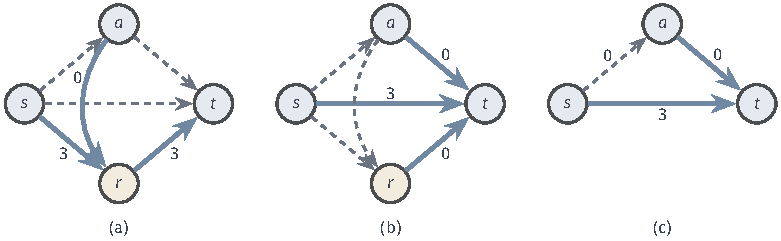
\includegraphics[width=132.186mm]{figures/01-basic-mathematics/04-graphs/tikz/c3-ns-artificial-start/figure.pdf}
  \caption{两阶段法的第一阶段。(a)人工根$r$（黄色）与人工弧构成星形可行树，人工流为$6$。(b)两次换基后人工流为零，$s\to t$承担$3$单位，空载的$r\to t$仍在树中。(c)删去人工结构，剩下的树弧构成原网络的生成树，作为第二阶段的初始树基。}
  \label{fig:graph-opt-ns-artificial-start}
\end{figure*}

人工流归零后删去人工根和全部人工弧。原来的树弧去掉人工弧后留下一个森林；在原图的每个弱连通分量内，用连接不同森林分量的原非树弧把它补成生成树。补入的弧保持原流量，作为树弧恰在界上是允许的。随后恢复原费用、重新计算势，并从所得的普通可行树基重新设置防循环数据，进入第二阶段。三点网络中删去$r$后，$s\to t$与$a\to t$已经构成生成树，$s\to a$在下界。

\paragraph{选入弧与沿环调整}
每一轮按以下步骤进行：
\begin{itemize}
  \item 定价：用当前势计算非树弧的约化费用。$L$中$\bar c_{i,j}<0$的弧应沿正向增加流量，$U$中$\bar c_{i,j}>0$的弧应沿反向减少流量；从这些违反条件的弧中选一条作为入弧。
  \item 找环：从入弧两端沿父指针上溯，深度大的一端先走，深度相同后一起走，相遇处是最近公共祖先；两段路径与入弧合成基本环。按入弧的调整方向给环定向，顺着定向经过的弧增加流量，逆着定向经过的弧减少流量。
  \item 求步长：增加的弧计算$u-x$，减少的弧计算$x-\ell$，入弧自身也参加比较，取最小值作为步长$\theta$。达到最小值的弧称为阻塞弧，可能不止一条，按防循环规则从中选出一条作为出弧。
  \item 更新流量：增加的弧加$\theta$、减少的弧减$\theta$，费用改变$\theta$乘以入弧在调整方向上的约化费用，$\theta>0$时严格下降。
  \item 更新树基：出弧是树弧时，它离开树，按到达的是下界还是上界归入$L$或$U$，入弧加入$T$，再更新父顶点、深度与势。出弧是入弧自身时，入弧在$L$与$U$之间翻转，树和势都不变。
\end{itemize}

\paragraph{退化、停止与输出}
步长为零的换基称为\term{退化换基}（degenerate pivot）。它发生在基本环上某条树弧已在阻塞方向的界上时：流量和费用不变，树基却变了。连续的退化换基可能在若干树基之间兜圈子，所以阻塞弧有多条时选哪一条必须写进算法。主流程采用适用于有界变量的\term{词典序规则}（lexicographic rule）：每个阶段开始时，在当时的可行树基上建立一致的符号扰动，比较阻塞量时连同扰动一起比较，并随换基更新扰动，完整构造见第~\ref{sec:graph-opt-ns-improvements}小节。任意选择或只取编号最小的阻塞弧都不能排除循环。

全部非树弧都满足符号条件，即$L$中$\bar c\geq0$、$U$中$\bar c\leq0$时，本阶段结束：第一阶段据人工流总量判定可行性，第二阶段返回原流、费用与势。

\begin{algorithm}[网络单纯形法]
\label{alg:graph-opt-network-simplex}
输入：有限有向网络，供需$b_i$，有限上下界与单位费用。输出：最优流$\bm x$、费用与节点势$\bm\pi$，或“不可行”。
\begin{enumerate}
  \item 平移下界、删去固定弧，记下常数$\bm c^{\top}\bm\ell$；在每个弱连通分量内检查剩余供需之和为零，否则报告不可行。
  \item 第一阶段：增加人工根与人工弧，取星形可行树基，原弧费用为零、人工弧费用为一，按当前树基设置词典序扰动。
  \item 以根为起点遍历树，求父顶点、深度与节点势，计算非树弧的约化费用；若没有违反符号条件的非树弧，转第6步。
  \item 选一条违反条件的入弧，构造基本环，比较环上各弧（含入弧）的剩余量得到步长$\theta$，按词典序规则选出出弧。
  \item 沿环更新流量；出弧是树弧时作树弧交换，否则作界翻转。回到第3步。
  \item 第一阶段停止时，若人工流总量为正，报告不可行；否则删去人工结构，在各分量内补成原网络的可行树基，恢复原费用并重新设置扰动，以第二阶段身份回到第3步。第二阶段停止时，把下界加回流量、常数加回费用，合并各分量的结果，返回流量、费用与节点势。
\end{enumerate}
\end{algorithm}

\paragraph{运行示例}
第一阶段结束后，三点网络的可行树基为$T=\{s\to t,a\to t\}$、$L=\{s\to a\}$，流量$(0,0,3)$，费用$12$，势$(\pi_s,\pi_a,\pi_t)=(4,1,0)$，即表~\ref{tab:graph-opt-ns-state}的状态。第二阶段的一轮如下，见图~\ref{fig:graph-opt-ns-pivots}(a)(b)：
\begin{itemize}
  \item 定价：$s\to a$在下界，$\bar c_{s,a}=1-4+1=-2<0$，正向入弧。
  \item 找环：$s$与$a$的父顶点都是$t$，基本环为$s\to a\to t$再逆着$s\to t$回到$s$；$s\to a$、$a\to t$增加，$s\to t$减少，正是“改走中转、减少直达”。
  \item 求步长：三条弧的剩余量依次为$3$、$2$、$3$，$\theta=2$，由$a\to t$唯一达到。
  \item 更新：流量变为$(2,2,1)$，费用下降$2\times2=4$，为$8$。$a\to t$到达上界，出树进入$U$；$s\to a$入树，$a$的父顶点改为$s$、深度变为$2$，顺着$s\to a$得$\pi_a=4-1=3$，势为$(4,3,0)$。
  \item 停止：唯一的非树弧$a\to t$在上界，$\bar c_{a,t}=-2\leq0$，即第~\ref{sec:graph-opt-mcf-optimality}节的证书。
\end{itemize}

把$s\to a$的容量改为$1$，从同一状态出发，$s\to a$仍正向入弧，剩余量变为$1$、$2$、$3$，步长$1$由入弧自身达到。于是作界翻转：$s\to a$从$L$转入$U$，树和势不变，流量$(1,1,2)$，费用$10$，见图~\ref{fig:graph-opt-ns-pivots}(c)。$s\to a$在上界而$\bar c_{s,a}=-2\leq0$，算法停止。两例只因入弧容量不同，阻塞弧一次是树弧、一次是入弧自身。

\begin{figure*}[!htb]
  \centering
  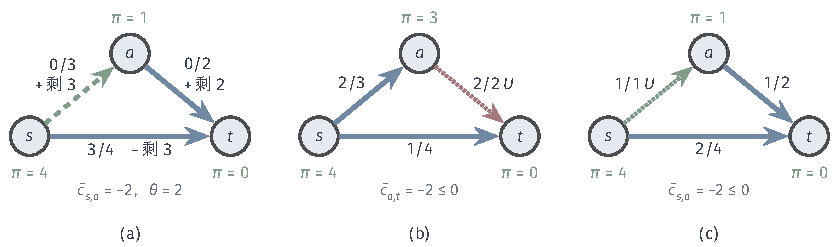
\includegraphics[width=142.053mm]{figures/01-basic-mathematics/04-graphs/tikz/c3-ns-pivots/figure.pdf}
  \caption{第二阶段的两种迭代。弧旁为流量/容量，“$\pm$剩”为沿基本环的剩余量。(a)$\bar c_{s,a}=-2$，最多推送$2$单位。(b)树弧$a\to t$出基进入$U$，费用$12\to8$。(c)$u_{s,a}=1$时入弧自身先到上界，树不变，费用$10$。}
  \label{fig:graph-opt-ns-pivots}
\end{figure*}

图~\ref{fig:graph-opt-ns-degenerate}在原网络上构造一次退化换基：把$s\to t$的容量改为$1$，从$T=\{s\to a,a\to t\}$、$U=\{s\to t\}$出发，流量$(2,2,1)$，树弧$a\to t$已在上界。以$t$为根，势为$(2,1,0)$，$s\to t$在上界而
\[
  \bar c_{s,t}=4-2+0=2>0,
\]
应反向进入；基本环上$a\to t$要增加流量，剩余量为$0$，所以$\theta=0$。

换基时$a\to t$出树进入$U$，$s\to t$入树，流量和费用不变而树基变了；新势$(4,3,0)$下$\bar c_{a,t}=-2\leq0$，算法停止。这次退化换基换来了证书，一般情形下连续退化则可能循环。

\begin{figure}[!htb]
  \centering
  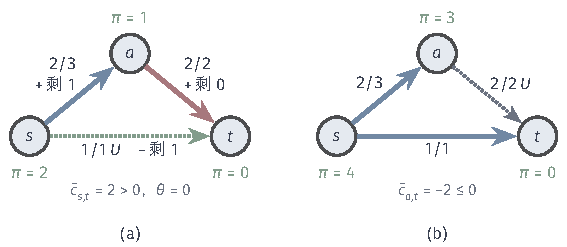
\includegraphics[width=96.054mm]{figures/01-basic-mathematics/04-graphs/tikz/c3-ns-degenerate/figure.pdf}
  \caption{退化换基（$u_{s,t}=1$）。(a)入弧$s\to t$（绿色）在上界且约化费用为正，反向进入；树弧$a\to t$（红色）剩余量为零，步长为零。(b)$a\to t$出基后流量与费用不变，新势满足最优性条件。}
  \label{fig:graph-opt-ns-degenerate}
\end{figure}

\subsection{正确性与复杂度}

三点改道可分三件事检查：仍送到$3$单位，不超容量，每单位费用降$2$。一般情形逐项对应：环上每个顶点一进一出，净流出不变；步长取环上剩余量的最小值，上下界仍满足；费用变化等于步长乘以入弧在调整方向上的负约化费用。

表示也保持合法：树弧交换删去的出弧在基本环上，删去后树仍连通无环，新的$T$仍是生成树，出弧落在它到达的界上，被正确归入$L$或$U$；界翻转只改变入弧的界状态。

树流由树基唯一确定，这可以用关联矩阵说明。按第~\ref{sec:graph-representations}节的约定，关联矩阵$\bm B$中弧$(i,j)$对应的列在第$i$行为$1$、第$j$行为$-1$，守恒式就是$\bm B\bm x=\bm b$。$\bm B$各行之和为零，删去根所在的一行不丢失信息，记剩下的矩阵为$\tilde{\bm B}$，树弧对应的列组成$(n-1)$阶方阵$\tilde{\bm B}_T$。

按消去叶子的次序排列行与列，每消去一个叶子，它所在的行在剩余树弧列中只有一个非零元，所以$\tilde{\bm B}_T$经重排后是对角元为$\pm1$的三角矩阵，从而可逆。于是树弧流量由
\begin{equation}
  \bm x_T=\tilde{\bm B}_T^{-1}\bigl(\tilde{\bm b}-\tilde{\bm B}_N\bm x_N\bigr)
  \label{eq:graph-opt-ns-tree-flow}
\end{equation}
唯一确定，其中$N=L\cup U$。

\begin{theorem}[网络单纯形法的正确性]
\label{thm:graph-opt-network-simplex}
在精确运算下，采用词典序规则的网络单纯形法在有限轮后停止。第一阶段最优人工流为零当且仅当原问题可行；可行时第二阶段输出的流是最小费用流，停止时的势与之构成最优性证书。若供需与上下界都是整数，输出的流为整数流。
\end{theorem}

\begin{proof}
有限终止：在一个阶段内，扰动后的供需固定不变，扰动后的流由树基唯一确定，所以扰动后的费用是树基的函数。词典序规则使扰动后的问题保持非退化，每轮扰动后的步长严格为正，扰动后的费用严格下降（第~\ref{sec:graph-opt-ns-improvements}小节证明），因此已出现过的树基不会再出现。$T$是有限多棵生成树之一，每条非树弧只有两种界状态，树基只有有限个，所以每个阶段在有限轮后停止。

可行性判定：若原问题有可行流，配上全零人工流就是第一阶段的可行解，目标为零，所以最优值为零；反之，最优值为零时人工弧全部空载，原弧流量满足原问题的全部约束。

最优性：每个阶段停止时树弧约化费用为零，非树弧满足所在界对应的符号条件，由定理~\ref{thm:graph-opt-potential-certificate}，当前流在本阶段的费用下最优。

整数性：初始星形树的流量是供需本身；树流由三角方程组逐叶解出，每步只做整数加减；步长是若干个整数剩余量的最小值，沿环更新仍是整数加减。所以每轮的流都是整数流。
\end{proof}

整数性为第~\ref{sec:graph-opt-mcf-unified}节的归约提供依据：只要可行，就存在整数最优流。第二阶段从清理后的树基重新设置扰动，有限终止的论证在两个阶段分别成立。

设顶点数为$n$，弧数为$a$。每轮扫描全部非树弧定价需要$O(a)$；沿父指针找基本环、比较剩余量、更新流量都是$O(n)$；沿新树重新求父顶点、深度与势也是$O(n)$。所以每轮主要操作为$O(n+a)$。

流量、界与费用的数组占$O(a)$，树记录与势占$O(n)$；词典序规则另为每条树弧存储$n-1$个扰动系数，共$O(n^2)$，每轮比较和更新这些系数也需$O(n^2)$。总开销还取决于迭代轮数，其中包括退化换基；有限性论证只给出与树基个数相当的上界，不能从单轮开销推出统一的多项式总时间界。

\subsection{实现改进与数值处理}
\label{sec:graph-opt-ns-improvements}

前面只说明了词典序规则怎样使用，下面补出它的完整构造，供需要时查阅。把上界写成等式$x_{i,j}+s_{i,j}=u_{i,j}$，$s_{i,j}\geq0$是上界松弛量。每条弧有两个离界距离$x_{i,j}-\ell_{i,j}$与$s_{i,j}$；只有每条树弧的两个离界距离都为正，步长才一定为正。词典序规则用符号扰动人为地制造这种非退化情形。

在一个阶段开始时，把当前可行树基的树弧编号为$e_1,\ldots,e_{n-1}$，把$e_k$的流量改为
\[
  x_{e_k}+\sigma_k\varepsilon^k,\qquad
  \sigma_k=\begin{cases}-1,& e_k\ \text{在上界},\\ +1,& \text{其他情形}.\end{cases}
\]
供需随之改为扰动后流量对应的净流出，并在整个阶段内保持不变；非树弧仍恰在界上。

$\varepsilon$是充分小的正数，每个量记为$(\text{常数},\varepsilon\text{的系数},\ldots,\varepsilon^{n-1}\text{的系数})$，从常数项起逐分量比较，即词典序比较。这样每条树弧的两个离界距离在词典序下都严格为正。

每轮比较步长时，增加流量的树弧以$u-x(\varepsilon)$为候选，减少流量的树弧以$x(\varepsilon)-\ell$为候选，入弧以$(u-\ell,0,\ldots,0)$为候选，取词典序最小者作为步长$\theta(\varepsilon)$并让它出基，所有树弧的扰动流量按$\theta(\varepsilon)$一同更新。

还原到基本环上，这个规则只在实际步长并列时起作用：比较并列阻塞弧的$\varepsilon$系数，选词典序最小者出基，实际流量仍按常数项更新。

以三点网络的第一阶段为例，按$s\to r$、$r\to t$、$a\to r$的次序设置扰动，三条树弧的流量为
\[
  3-\varepsilon,\qquad 3-\varepsilon^2,\qquad \varepsilon^3.
\]
$s\to t$入树时，$s\to r$与$r\to t$的候选向量为
\[
  (3,-1,0,0),\qquad (3,0,-1,0),
\]
前者更小，所以$s\to r$出基。

\begin{proof}[词典序规则保持非退化的证明（补充阅读）]
初始时各树弧的$\varepsilon$系数行是$\pm$单位向量，线性无关。每次树弧交换，留下的树弧系数行加减出弧的系数行，入弧取出弧系数行的正负，这是可逆的行变换；界翻转不改变系数行。所以树弧的系数行始终线性无关，两条树弧的候选向量不会相等，入弧的候选向量只有常数项，也不会与树弧的相等，词典序最小者唯一。更新后出弧恰好落在界上，其余树弧仍在词典序下严格离界，扰动后的问题始终非退化，每轮的$\theta(\varepsilon)$在词典序下严格为正。扰动后的费用改变量为$\theta(\varepsilon)$乘以负的约化费用，因而严格下降。
\end{proof}

另一类常用规则维护所谓强可行树，有自己的方向约定与初始化要求；第一阶段清理只得到普通的可行树基，两类规则不能混用。

常见的实现改进只改变维护代价，不改变可行性与最优性条件。一是局部更新势：删去出弧后树分成两块，只有不含根的一块的势同加或同减入弧的约化费用，只需遍历这棵子树。二是按先序后继与子树大小存储树，换基时只重排被移动的子树。三是分块定价：每轮只扫描一部分非树弧，找到违反条件的弧就入树。

找环、界翻转和子树更新的写法可以对照NetworkX库中的网络单纯形实现\scite{math-graph-networkx-network-simplex}，但它的初始化与防循环规则另有前提，不能与本章的两阶段词典序版本混用。

精确整数数据下，上述判断都能精确进行。浮点实现中，守恒、弧界、约化费用的符号与步长比较都只能在容差内判断，例如把绝对值小于容差的约化费用当作零；容差过小会因舍入反复选弧，过大会漏掉改进方向。

有限容量的主线不会出现费用无界。若扩展到无穷容量，还须处理增加方向剩余量全为无穷的基本环：这时步长无穷而入弧约化费用为负，存在可以无限推送的负费用环，应报告费用无下界。

\section{最大流、匹配与指派的统一表示}
\label{sec:graph-opt-mcf-unified}

第~\ref{chap:max-flow-min-cut}章与第~\ref{chap:bipartite-matching-assignment}章的问题都能写成最小费用流。最大流的流值不固定，不能直接写成供需，办法是令全部$b_i=0$，原弧费用为零，再加一条从$t$回到$s$的回边，容量取源点原出弧容量之和，费用为$-1$。

下面说明这个循环流模型与最大流一一对应。对任一循环流，由源点守恒，$s$经原弧的净流出等于回边流量$x_{t,s}$，即原网络的源汇流值，总费用为它的相反数。反过来，值为$v$的流配上$x_{t,s}=v$就是循环流，$v$不超过源点出容量，回边容量够用。

于是最小费用循环流对应最大流，最小费用就是负的最大流值。只设零费用而不加回边则不够：全零流已是最优。

二部最大匹配沿用第~\ref{sec:graph-opt-match-alternating}小节的单位容量网络：$s$连向左侧各顶点，允许边从左指向右，右侧各顶点连向$t$，容量都是$1$、费用为零，再加入上述费用为$-1$的回边，容量取两侧顶点数的较小者。由定理~\ref{thm:graph-opt-network-simplex}的整数性，存在整数最优循环流，其中间弧上流量为$1$的弧两两不共享端点，构成匹配，配对数等于回边流量；反之每个匹配都给出这样的循环流，所以费用最小等同于配对数最多。

$r$阶指派在同一个单位容量配对网络中固定输送量$r$：令$b_s=r$、$b_t=-r$，中间弧的费用为配对成本$c_{i,j}$，其余弧费用为零，不加回边。整数可行流使每个左侧顶点恰送出一单位、每个右侧顶点恰收到一单位，对应一个完美匹配，总费用就是指派成本。

由整数性，只要可行就存在整数最优流，它给出最优指派；若送不出$r$单位，说明不存在完美匹配，指派不可行。若要最大化收益，费用取收益的相反数；矩形问题按第~\ref{sec:graph-opt-assign-rectangular}小节补成方阵后写入网络，求解后删去虚拟配对。

图~\ref{fig:graph-opt-problem-relations}汇总了这些关系。最小费用流保留了一般的容量与供需；最大匹配只求配对数量，指派在完整配对的条件下比较成本。

专门算法利用各自的结构：最大流算法只沿源汇方向增广，匈牙利算法与Hopcroft--Karp算法只记录配对伙伴，KM算法的标号与Auction算法的价格是二部图上的节点势。统一表示说明问题可以转化，并不意味着网络单纯形法在所有输入上都优于专门算法。

\begin{figure}[!htb]
  \centering
  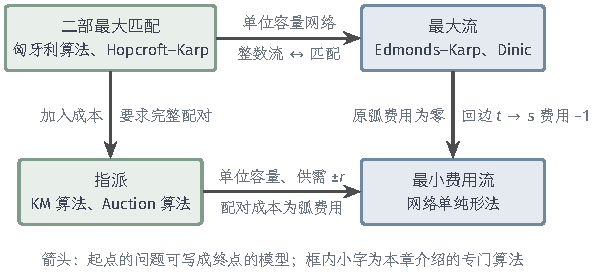
\includegraphics[width=101.829mm]{figures/01-basic-mathematics/04-graphs/tikz/c3-problem-relations/figure.pdf}
  \caption{本章四种流与配对问题之间的模型关系。箭头表示起点的问题可以写成终点的模型：二部最大匹配是单位容量的最大流，加入成本并要求完整配对就成为指派；最大流加入费用为$-1$的回边后成为最小费用循环流；指派是供需为$\pm r$的单位容量最小费用流。框内小字是本章介绍的专门算法。}
  \label{fig:graph-opt-problem-relations}
\end{figure}

\section{结果检验}
\label{sec:graph-opt-ns-analysis}

输出须回到原始问题检查，因为算法求解的是平移下界、删去固定弧之后的问题。先把下界平移量加回流量，核对每个顶点的净流出等于原始$b_i$、每条弧满足原始上下界；再按原始费用重算目标值，确认它等于平移后问题的费用加上常数$\bm c^{\top}\bm\ell$。被删去的固定弧要按其固定流量补回，它们的费用已计入这个常数。

最优性用输出的势逐弧核对条件~\eqref{eq:graph-opt-mcf-certificate}，核对时使用原始上下界。平移不改变约化费用，也不改变一条弧是否在界上：$y_{i,j}=0$当且仅当$x_{i,j}=\ell_{i,j}$，$y_{i,j}=u_{i,j}-\ell_{i,j}$当且仅当$x_{i,j}=u_{i,j}$。

以图~\ref{fig:graph-opt-mcf-lower-bound}的下界版本为例，平移后问题的最优解$\bm y=(2,2,0)$加回下界得$\bm x=(2,2,1)$。三个顶点的守恒核对如下：
\[
  \begin{aligned}
    s\ \text{净流出}&:\ 2+1=3,\\
    a\ \text{净流出}&:\ 2-2=0,\\
    t\ \text{净收进}&:\ 2+1=3.
  \end{aligned}
\]
各弧都在原始界内；原始费用$2+2+4=8$，等于平移后的费用$4$加常数$4$。

再用势$(4,3,0)$核对符号条件，三条弧的状态与约化费用为
\[
  \begin{aligned}
    s\to a\ \text{严格在界内}&:\ \bar c_{s,a}=1-4+3=0,\\
    a\to t\ \text{在上界}&:\ \bar c_{a,t}=1-3+0=-2\leq0,\\
    s\to t\ \text{在下界}&:\ \bar c_{s,t}=4-4+0=0\geq0.
  \end{aligned}
\]
其中$s\to t$的流量$1$恰为下界。与无下界的原例相比，$s\to t$从“界内”变成了“在下界”，要求的符号随之改变，所以核对必须按原始上下界逐弧判断。

可行性与最优性分别验收：前者只看流，后者还要看势。浮点结果应分别报告守恒误差、弧界违反量与约化费用符号的误差；在容差内近似满足的条件不能当作精确证书。

\section{其他改进路线}
\label{sec:graph-opt-mcf-other-methods}

网络单纯形法不是求最小费用流的唯一方法。各种方法都以第~\ref{sec:graph-opt-mcf-optimality}节的条件为终点：残量网络中没有负费用环，或者等价地，存在一组使全部残量弧约化费用非负的势。它们的差别在于运行中始终保持哪一半条件。一类方法始终保持流可行，逐步消除负费用环；另一类始终保持约化费用非负，逐步满足供需。下面简述三条路线的思路、所需条件与复杂度量级，系统的讲述可参考Bertsekas的网络优化教材\scite{math-graph-bertsekas1998network}。本章正文完整展开的仍是网络单纯形法。

\paragraph{负环消去}
负环消去直接执行定理~\ref{thm:graph-opt-negative-cycle}。先求一个可行流：加入超级源$s^\ast$与超级汇$t^\ast$，从$s^\ast$向每个供给点$i$连容量为$b_i$的弧，从每个需求点$i$向$t^\ast$连容量为$-b_i$的弧，用第~\ref{chap:max-flow-min-cut}章的方法求最大流；最大流把这些新弧全部送满时，原弧上的流量就是可行流，否则问题不可行。

随后反复在费用残量网络中寻找负费用环，沿环推送环上的最小剩余容量$\theta>0$，费用下降$\theta\,|c(C)|$。为了不漏掉任何负环，先像第~\ref{sec:graph-opt-mcf-optimality}节那样加入一个向全部顶点连零费用弧的虚拟源点，再用第~\ref{sec:graph-opt-bellman-ford}节的Bellman--Ford算法在$O(na)$时间内判断有无负环。

报告负环时，对一条仍可改善的弧再松弛一次，从其终点沿前驱指针回退$n$步，就落在前驱指针形成的一个环上；第~\ref{sec:graph-opt-bellman-ford}节的路线恢复论证说明，这样的环费用为负。找不到负环时，由定理~\ref{thm:graph-opt-negative-cycle}，当前流最优。

费用与容量都是整数时，每次推送使费用至少下降$1$。记$C=\max|c_{i,j}|$、$U=\max u_{i,j}$，任一可行流的费用绝对值不超过$aCU$，所以消环次数不超过$2aCU$，总时间为$O(na^2CU)$。这个界随数值增长，是伪多项式的；任意选环时实际次数也可能很多。

网络单纯形法可以看成只在当前树的基本环中找负环：定价只需$O(a)$，代价是可能出现步长为零的退化换基，而负环消去在残量网络中推送的步长总为正。

\paragraph{逐次最短路}
逐次最短路从另一半条件出发。它维护一个满足上下界、但未必满足供需的流$\bm x$，以及一组使全部残量弧约化费用非负的势$\bm\pi$。顶点$i$的剩余供给记为
\[
  e_i=b_i-(\text{$i$在$\bm x$下的净流出}),
\]
$e_i>0$表示还要送出，$e_i<0$表示还要收进。

初始取$\bm x=\bm 0$。若全部费用非负，取$\bm\pi=\bm 0$即可；若有负费用弧但没有负费用环，可按第~\ref{sec:graph-opt-mcf-optimality}节的办法用最短距离构造势；一般情形可以先把负费用弧送满，使它们只留下费用为正的反向残量弧，再相应修改$e_i$。

每一轮取一个$e_k>0$的顶点$k$，在残量网络中以约化费用为长度求从$k$出发的最短距离$d_i$。约化费用非负，所以可以用第~\ref{sec:graph-opt-dijkstra}节的Dijkstra算法。

若从$k$到达不了任何$e_i<0$的顶点，问题不可行：从$k$可达的顶点集$R$没有离开它的残量弧，即离开$R$的原弧都已满载、进入$R$的原弧都为零，当前流已从$R$送出了可能的最大净量。$R$中没有剩余需求，各顶点的$e_i$都非负，而$e_k>0$，所以任何满足供需的流都要从$R$送出比这更多的净量，不可能做到。

否则取一个可达的$e_\ell<0$的顶点$\ell$，按
\begin{equation}
  \pi_i\gets\pi_i-d_i
  \label{eq:graph-opt-ssp-potential-update}
\end{equation}
更新势；不可达顶点的$d_i$取为可达顶点距离中的最大值。

对残量弧$i\to j$，更新势后的约化费用为
\[
  \bar c_{i,j}+d_i-d_j.
\]
两端都可达时由最短距离的三角不等式非负；$i$不可达而$j$可达时，$d_i$取最大值，同样非负；两端都不可达时不变；$i$可达而$j$不可达的残量弧不存在。于是新势仍使全部约化费用非负，并且$k$到$\ell$的最短路径上每条弧的约化费用都变为零。

沿这条路径推送
\[
  \theta=\min\{e_k,\ -e_\ell,\ \text{路径上的最小剩余容量}\}.
\]
推送产生的反向残量弧，约化费用是路径弧约化费用的相反数，也是零，所以条件继续保持。全部$e_i=0$时，流可行且全部残量弧约化费用非负，由定理~\ref{thm:graph-opt-negative-cycle}最优。

整数数据下每轮至少推送一单位，轮数不超过初始剩余供给之和$B=\sum_{e_i>0}e_i$；用二叉堆实现Dijkstra算法时，总时间为$O(B(n+a)\log n)$，同样随数值增长。按容量缩放、每个阶段只沿剩余容量足够大的路径成批推送的变体，可以把对$B$的线性依赖换成对容量上界的对数依赖。

在指派网络上，$B=r$，逐次最短路每轮为一行完成配对，并用势保持约化费用非负；这与KM算法逐行增广、用可行标号保持剩余量非负的做法相对应。

\paragraph{费用缩放}
第三条路线放宽最优性条件。若全部残量弧的约化费用都不小于$-\varepsilon$，称流$\bm x$与势$\bm\pi$满足$\varepsilon$最优性。

费用为整数且$0<\varepsilon<1/n$时，$\varepsilon$最优已经推出最优。任一残量环$C$至多含$n$条弧，环的费用等于约化费用之和，于是
\[
  c(C)=\sum_{(i,j)\in C}\bar c_{i,j}\geq-n\varepsilon>-1.
\]
而$c(C)$又是整数，只能非负，于是没有负费用环。

费用缩放从$\varepsilon=C$开始，每个阶段把$\varepsilon$减半，并用沿残量弧的局部推送与调整势恢复$\varepsilon$最优性，直到$\varepsilon<1/n$。这样的算法可以得到关于$n$、$a$和$\log(nC)$的多项式时间界，总时间只以对数形式依赖费用范围。第~\ref{sec:graph-opt-auction}小节的$\varepsilon$互补松弛与$\varepsilon$缩放正是这一思想在指派问题上的形式：那里的误差界$r\varepsilon$与这里的$-n\varepsilon$下界出自同一个求和论证。

三条路线与网络单纯形法使用同一个残量结构和同一份最优性证书，差别在于维护什么、多久完成。比较时应说明数据是否为整数、复杂度依赖哪些数值，以及界是最坏情形还是经验表现；任何一种方法停止后，都可以用第~\ref{sec:graph-opt-ns-analysis}节的检验核对结果。

\FloatBarrier
\section{本章小结}
\label{sec:min-cost-flow-summary}

章首的第一个问题是怎样建模。最小费用流给每个顶点一个供需量，给每条弧上下界与单位费用，在全部满足守恒与上下界的流中最小化总费用。供需之和为零只是可行的必要条件；正下界通过平移化为零，平移带来的常数费用必须在最后恢复。容量有限时，可行流集合闭有界，只要可行就一定取到最小费用。

第二个问题是怎样判断最优。任何两个可行流之差都能拆成残量环的叠加，所以可行流最优当且仅当费用残量网络中没有负费用环。环的个数可能很多，节点势把这一条件改写为逐弧可查的证书：界内弧约化费用为零，下界弧非负，上界弧非正。没有负环时，由虚拟源点出发的最短距离总能给出这样的势。

第三个问题是怎样逐步改进。网络单纯形法把可行流记在树基上，用树弧约化费用为零确定势，以非树弧的约化费用定价，沿基本环推送到某条弧碰界再换基。两阶段法用人工根判定可行性，词典序规则排除退化换基造成的循环；数据为整数时输出整数流，这为把最大流、二部图匹配和指派写成最小费用流提供了依据。每轮开销为$O(n+a)$，但总轮数没有统一的多项式界。负环消去、逐次最短路与费用缩放用同一份证书组织不同的改进，统一表示也不意味着网络单纯形法在所有输入上都优于专门算法。

回看整个部分，各问题选择的对象、依靠的论证与停止时留下的证书各不相同，表~\ref{tab:graph-opt-summary}把它们并列。证书的价值在于检查者不必相信求解过程，只需核对可行性和若干不等式；但证书只在其条件下成立，例如Auction算法的价格只给出误差界，整数成本且$\varepsilon<1/r$时才是精确最优。浮点计算中的核对都要带容差，近似满足不能直接当作精确证书。

\begin{table*}[!htb]
  \centering\small
  \caption{本部分六个问题的对比（$n$为顶点数，$m$为无向边数，$a$为有向弧数，$p$为二部图较小一侧的顶点数，$r$为指派方阵的阶数，$B$为Auction算法的竞价次数）。开销均为本部分所述实现的运算量。}
  \label{tab:graph-opt-summary}
  \begin{tabularx}{\linewidth}{@{}l>{\raggedright\arraybackslash}X>{\raggedright\arraybackslash}X>{\raggedright\arraybackslash}X>{\raggedright\arraybackslash}p{30mm}@{}}
    \toprule
    问题 & 选择对象与目标 & 方法与成立条件 & 结果证书 & 主要开销\\
    \midrule
    最短路 & 一条路径，弧长之和最小 & DAG递推（无有向环）；Bellman--Ford（允许负边，检测负环）；Dijkstra（可达部分边长非负） & 逐弧距离不等式与前驱路线 & $O(n+a)$；$O(na)$；$O((n+a)\log n)$\\
    最小生成树 & 连接全部顶点的边集，成本之和最小 & Kruskal、Prim，依靠割性质 & 无环、覆盖各分量；非树边不轻于树上对应路径的边 & $O(m\log n)$；$O(n^2+m)$或$O((n+m)\log n)$\\
    最大流 & 各弧流量，源汇净输送量最大 & 残量增广；Edmonds--Karp按最少弧数选路，Dinic分层求阻塞流 & 同值的流与割 & $O(na^2)$；$O(n^2a)$\\
    二部最大匹配 & 互不共享端点的边，边数最多 & 交替路径增广（匈牙利算法），Hopcroft--Karp分层成批增广；限于二部图 & 无增广路径，或单位容量网络中同值的割 & $O(n+pm)$；$O(n+m\sqrt n)$\\
    指派 & 完美匹配，成本之和最小 & KM：可行标号、紧边交替树与调标；Auction：价格与竞价，完整有限成本矩阵 & 成本等于标号之和；$\varepsilon$条件与误差界$r\varepsilon$ & $O(r^3)$；$O(r^2+rB)$\\
    最小费用流 & 各弧流量，供需固定时费用最小 & 网络单纯形法：可行树基、基本环调整、两阶段初始化、词典序防循环 & 流量与节点势的逐弧符号条件 & 每轮$O(n+a)$，总轮数无统一多项式界\\
    \bottomrule
  \end{tabularx}
\end{table*}

本部分选择的始终是路径、树、流、匹配这类具有特定组合结构的对象，算法的正确性也来自这些结构本身的性质。下一部分转而用集合函数评价一般的子集，候选对象可以是图的顶点、边，也可以是传感器。那里将区分两种情形：一种是评价函数的一般性质，如收益递减，给出贪心选择的近似保证；另一种是特殊的表示，如可以写成图割，带来精确的求解。

